\documentclass[12pt,a4paper,leqno]{report}

\usepackage[utf8]{inputenc}
\usepackage[T1]{fontenc}
\usepackage[english]{babel}
\usepackage{amsthm}
\usepackage{amsfonts}         
\usepackage{amsmath}
\usepackage{amssymb}
\usepackage{enumerate}
\usepackage{hyperref}
\usepackage{booktabs}
\usepackage{array}
%\usepackage{dsfont}
\usepackage{lmodern}
\usepackage{scrextend}
\usepackage{tikz}
\usepackage[colorinlistoftodos]{todonotes}
\usepackage{graphicx}
\usepackage{capt-of}
\usepackage{makeidx}
\usepackage[
backend=biber,
style=authoryear-icomp,
citestyle=authoryear,
maxcitenames = 1,
uniquelist = false
]{biblatex}

\newcolumntype{L}[1]{>{\raggedright\let\newline\\\arraybackslash\hspace{0pt}}m{#1}}

\newcommand{\R}{\mathbb{R}}
\newcommand{\C}{\mathbb{C}}
\newcommand{\Q}{\mathbb{Q}}
\newcommand{\N}{\mathbb{N}}
\newcommand{\No}{\mathbb{N}_0}
\newcommand{\Z}{\mathbb{Z}}
\newcommand{\diam}{\operatorname{diam}}
\newcommand{\F}{\mathcal{F}}
\newcommand{\dif}{\,\mathrm{d}}
\newcommand{\sijoitus}[2]{\mathop{\Big/}\limits_{\hspace{-0.85em}{#1}}^{\hspace{0.85em}{#2}}\hspace{-0.2em}}
\newcommand{\var}{\mathrm{Var}}
\newcommand{\cov}{\mathrm{Cov}}
\newcommand{\corr}{\mathrm{Corr}}
\def\independent{\perp\!\!\!\perp}

\theoremstyle{plain}
\newtheorem{lause}[equation]{Theorem}
\newtheorem{lem}[equation]{Lemma}
\newtheorem{prop}[equation]{Proposition}
\newtheorem{kor}[equation]{Corollary}

\theoremstyle{definition}
\newtheorem{defin}[equation]{Definition}
\newtheorem{maar}[equation]{Definition}
\newtheorem{konj}[equation]{Conjecture}
\newtheorem{esim}[equation]{Example}

\setcounter{chapter}{-1}
\renewcommand{\theequation}{\thechapter.\arabic{equation}}

%\theoremstyle{remark}
\newtheorem{remark}[equation]{Remark}

\pagestyle{plain}
\setcounter{page}{1}
\addtolength{\hoffset}{-1.15cm}
\addtolength{\textwidth}{2.3cm}
\addtolength{\voffset}{0.45cm}
\addtolength{\textheight}{-0.9cm}

\title{Introduction to Probability}
\author{Ville Hyvönen, Patrik Lauha, Topias Tolonen\thanks{This material is strictly based on the Finnish material Todennäköisyyslaskenta I (2018) by Ville Hyvönen, Patrik Lauha and Topias Tolonen, and translated and updated by Topias Tolonen in early 2020. Special thanks to Ville and Patrik, and in addition to Mika Koskenoja for providing examples, exercises and guidance. Suggestions, comments and errors are continuously accepted at $topias.tolonen@helsinki.fi$.}}

\date{April 15th, 2020}

\makeindex

\addbibresource{ref.bib}

\begin{document}

\maketitle

\tableofcontents

%%%%%%%%%%%%%%%%%%%%%%%%%%%%%%%%%%%%%%%%%%%%%%%%%%%%%%%%%%%%%%%%%%%%%%%%%%%%%%%%

\chapter{Introduction}\label{intro}

\section{Foreword}

Firstly, thank you for reading this material. It is designed to serve as a course material for the introduction level probability course within the University of Helsinki. This material is written in a way where a student without notable background in university-level mathematics, together with a suitable set of exercise sets, can grasp the basic concepts of elementary probability. Of course, the material is best served with a $5$ ECTS course, but we are doing our best to write a material so exhaustive and complete that it would be possible to learn the contents of this material by self-studying.

For a long time, the students within the University of Helsinki took the introductory class to probability together with the famous textbook \textcite{Tuominen2010}, which had an extensive albeit theory-heavy approach to the concepts of probability. During the years 2016--2019 a new Finnish course material began to develop itself: first by Ville Hyvönen, then updated by Topias Tolonen, and later rewritten in 2018 by Patrik Lauha, together with Tolonen and Hyvönen. During this process, the exercices and insights provided by Mika Koskenoja were invaluable. \textcite{Lauha} was based on the excellent book \textcite{Ross} and the lecture notes of \textcite{Koistinen2013}, together with small hints of \textcite{Stirzaker}. This material will thus follow the same suit. 

By the time of writing this, the Finnish version of this material has been used as a textbook in a total of three lectured courses by either Mika Koskenoja or Topias Tolonen, and the English version -- which you are currently reading -- has been used and tested once in a lectured course by Mika Koskenoja. During these courses, the material has been updated and mistakes have been fixed, based on feedback by active students. We are grateful for every student who has had the courage and willingness to point out errors in our material.

As I mentioned before, the material will provide an extensive basis for probability\footnote{Note, however, that this material will not be covering anything referred to as \emph{probability theory}, which is a measure theoretic approach for probability and often saved for more advanced students. An excellent resource for this approach is, for example, \textcite{durrett}.}, and it does not have many prerequisites: the most notable would be a requirement for a upper secondary, or high school, level of calculus. Familiarity with mathematical concepts, such as proofs, definitions and lemmas ought to be useful, as is the knowledge of elementary set theory\footnote{Which will, however, be reviewed in the chapter \ref{chap1}.}. However, I would not worry about these things too much at this point. Let's get to the basics! 

Again, sincerely, hope this material helps you with the concepts of probability and sparks you with the interest to studying the subject of probability and statistics further.\linebreak

April 2020, Topias Tolonen

\section{What do we Mean by Probability?}

\emph{This section is meant to nudge the student to think about the concept of probability. How would you interpret the meaning of the sentence 'In Helsinki, there will be rain tomorrow with a probability of $0.5$'?}

Probability is a subfield of mathematics, which is used to observe, examine and control a concept called \emph{randomness}. It is applied in a various fields of science, such as statistics, natural sciences, economics, finance and data science. Even though the field of probability has been developed as early as the 17th century, the possibilities it provides have lately notably expanded due to the remarkable improvements in computing power.

The history of probability is closely tied with gambling: French writer and an avid gambler Chevalier de Méré noticed following during the 17th century: \index{de Méré's problem}

\begin{itemize}
    \item When tossing dice four times, it is profitable to bet that at least one of them turns out to be a number $6$.
    \item When tossing dice 24 times, it is not profitable to bet that at least one pair of $6$'s shows up.
\end{itemize}

However, de Méré could not proof these insights. Instead he asked his friend, mathematician Blaise Pascal for help. Pascal solved the problem together with his acquaintance Pierre de Fermat and thus built the foundation for the theory of probability. Later on, the field of probability was notably advanced by the pioneers Jakob Bernoulli, Abraham de Moivre and Pierre Simon de Laplace. For the longest time, the theory of probability was only understood through \emph{combinatorics} and so-called \emph{classical definition of probability}\footnote{See sections \ref{komb} and \ref{classprob}}, until a mathematician Andrei Kolmogorov introduced the \emph{axioms of probability}\footnote{See the definition \ref{maar:prob}.}, which act as an exact mathematical definition for something we regard as 'probability'.

In these modern times, the applications for probability extend well beyond the reach of gambling. The art of examining randomness is used far and wide in industries and other applications to \emph{model} and control uncertainty: if one receives numbers that represent the behaviour of random phenomena, they also receive numbers that represent uncertainty. This enables a rational discussion regarding uncertainty, and furthermore it enables a comparison for different alternatives. The skill to control the uncertainty and to manage risks is a vital skill, especially in the 21st century where we can effortlessly model surprisingly complex phenomena. For example, artificial intelligence and machine learning have their foundations built deep in the area of probabilities. In addition to those, for example finance as a field is heavily dependant on the possibilities brought by the field of probabilities, whether the mathematics was used to manage portfolio risk or to forecast the derivatives market. To model the uncertainty is to model the future.

Now, let's get back to the original question of this section: \emph{How would you interpret the meaning of the sentence 'In Helsinki, there will be rain tomorrow with a probability of $0.5$'?}

Before all else, let us state that a probability is not a physical measurement like height or weight of an object -- you are not able to measure a probability of some item or some event by measuring their physical attributes. For probabilities, you need to be more creative.

There are multiple ways to define probabilities, and to begin, we need to examine the \emph{meaning} or \emph{interpretation} behind the concept of probability. To begin, let us clear out the trivial case and state that some \emph{events} or phenomena are \emph{deterministic} -- by this we mean that the end result of such event can surely be deduced from large enough set of information concerning the said event. For example, we could argue that the process of a snowball melting is deterministic: when the snowball is brought indoors, it will melt following the thermodynamical process defined by the laws of physics. Eventually, the snow will reach zero degrees Celcius and melt into water. There are no random activities going on out here: we can calculate the exact point where the snow has turned into water by knowing the amount of snow, the melting point of snow and the indoor temperature\footnote{In this illustrative example, we most likely would need some more parameters thrown in: the indoor humidity, and other such factors. However, the point stands -- when we know enough information about the snow, the room, and other factors, we are able to calculate every step of the melting process.}.

However, all events are not deterministic. In fact, very few are. A traditional example of a non-deterministic, \emph{random}, event would be a toss of an unweighted die. We are not able to state the end result of the toss beforehand: we are only able to state the possible results of the toss, and if we are lucky, how likely each event is. Before examining the mathematical definition of probability\footnote{See chapter \ref{math.prob}.}, let us shortly discuss the different interpretations to the concept of probability

To put it simply, the meaning of probability is to measure how strongly one believes that the claim is either true of false. When we claim that the probability of rain is $0.5$, we argue that from our perspective, the possibility for rain tomorrow is equally likely to the possibility of a clear sky. In the beforementioned example of dice toss represents the classical interpretation of probability, where we consider each possible event equally likely -- that is, the probability of each of these events is equal. In classical probability we define the probability simply as the ratio of the ''succesful'' events and all possible events. For example, in a die toss a probability of an even number is $\frac{3}{6}$: there are six different possible outcomes, of which three represent even numbers.

In many occasions, all possible events are not equally likely and thus the classical interpretation of probability can not be used. An example of this kind of situation would be presidential elections, where person $A$ runs against person $B$. Before the election night somebody might claim that $A$ has $70\%$ chance to win the elections. In such situation, the probability is used as a measurement for the ''chance'' that said event happens, and furthermore it is at least sometimes a subjective interpretation on the realisation of different outcomes of a random event. In a once-in-a-lifetime events such as elections it is difficult to judge whether the probabilities given before the election night were right or wrong -- information about the outcome, say, person $B$ winning the election despite the odds, does not in itself tell anything about the ''validity'' of the probabilities given, or what the ''true'' probabilities were. In addition, we can extend the setting in a following way: let the person claiming $70\%$ chance for $A$'s victory gain more information: she finds out that a huge scandal is going to erupt and pummel the public opinion on $A$, and she updates her forecast that given the scandal. She now claims that $A$ has only $45\%$ chance to win -- most often we call this kind of subjective probability, where we are able to update our probability given data, a \emph{Bayesian interpretation of probability.}

In contrast, there are events that can, unlike a presidential election, be repeated, or where a similar forecast is continuously provided. In these kinds of events, we are able to empirically examine the validity of the forecasts and the ''true'' probabilities of these events. For example, we are able to examine the success of weather forecasts by comparing the forecasts to the weathers that occurred. If we select all past forecasts which claim $90\%$ chance for rain next day and examine the actual weather of the next day, and we would want to argue that the forecasts are correct, it would make sense to require approximately $9$ out of $10$ days to be rainy. The kind of probability required for this kind of inference is called the \emph{frequentist interpretation of probability}, where the probability is interpreted through the frequency of ''successful'' events, is essential to the art of statistical inference. The interpretation of probabilities through the frequences of the events are further discussed in the chapters \ref{toistokokeet} and \ref{sll}. 

The purpose of this material is to help the student to understand the principles behind the field of probability and to calculate probabilities of given events. During this material, the student will revise combinatorics and elementary set theory and learn the basic concepts of probability, random variables and most common probability distributions. In addition, the student will learn to interpret the probability distributions with different statistics and to familiarize herself with the most central laws in the theory of probability.

%%%%%%%%%%%%%%%%%%%%%%%%%%%%%%%%%%%%%%%%%%%%%%%%%%%%%%%%%%%%%%%%%%%%%%%%%%%%%%%%

\chapter{Reviewing Set Theory and Combinatorics}\label{chap1}

In this material we are going through some mathematical expressions and concepts, which include sets and their elements. Sets are handled with a subfield of mathematics called \emph{set theory}, and the number of elements in each set are counted with the help of \emph{combinatorics}. In this chapter, we are going to review some mathematical notation, set theory and combinatorics, which are essential in learning the field of probability.

\section{The Basic Concepts of Elementary Set Theory}

\emph{In this section we briefly introduce and review those core concepts of set theory which are relevant for the scope of this material.}

As stated in the previous chapter, probability is much based on set theory. Let us start with establishing key notations. A \emph{set}\index{Set} is a non-ordered collection of any kind of objects, which we call \emph{elements}\index{Set!Element}. Let $A$ and $B$ be some arbitrary sets and let $x$ be an arbitrary element. In such setting, following notations are widely used for the most common \emph{set operations}\index{Set!Set operation}:

\bigskip

\begin{tabular}{l l }
\toprule
Notation & Meaning \\
\midrule
$x \in A$  & Element $x$ \emph{is a member} \index{Set!Membership} of a set $A$ (also used: \emph{$x$ is an element of $A$})\\
$x \notin A$ & Element $x$ \emph{is not a member} of set $A$ \\
$A^C$ & \emph{Complement} of set $A$,\index{Set!Complement} that is, the elements not in the set $A$ \\
$A = B$ & $A$ and $B$ are \emph{equal},\index{Set!Equality}, that is, they include exactly the same elements\\
$A \subset B$ & $A$ is the \emph{subset} of $B$,\index{Set!Subset} that is, all elements of $A$ are also members of $B$. \\
$A \subseteq B$ & $A$ is the subset of $B$, and in addition, the sets may be equal $A=B$.\\
$A \cup B$ & \emph{Union}\index{Set!Union} $A$ and $B$ $\{x\colon x \in A \text{ or } x \in B\}$ \\
$A \cap B$ & \emph{Intersection}\index{Set!Intersection} of $A$ and $B$ $\{x\colon x \in A \text{ and } x \in B\}$\\
$A \setminus B$ & \emph{Set difference}\index{Set!Set difference} of $A$ and $B$  $\{x \colon x \in A \text{ and } x \notin B\}$ \\
$\emptyset$ & \emph{Empty Set}\index{Set!Empty set} \\
\bottomrule 
\end{tabular}
\bigskip

These set operations can be easily illustrated with so-called Venn diagrams:

\begin{figure}[!h]
\centering
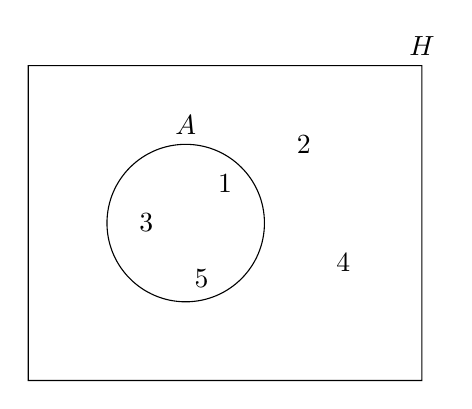
\begin{tikzpicture}[fill=gray]
\draw (0,0) circle (1) (0,1)  node [text=black,above] {$A$}
	  (0.5,0.5) node [text=black] {$1$}
      (-0.5,0) node [text=black] {$3$}
      (0.2,-0.7) node [text=black] {$5$}
      (1.5,1) node [text=black] {$2$}
      (2,-0.5) node [text=black] {$4$}
      (-2,-2) rectangle (3,2) node [text=black,above] {$H$};
\end{tikzpicture}
\caption{Natural numbers 1, 2, 3, 4 and 5 make up a set $H$. The set $A$, consisting of numbers 1, 3 and 5, is a subset of $H$. Now, we can state $1 \in A$ and $5 \in H$.} 
\end{figure}

\begin{figure}[!h]
\centering
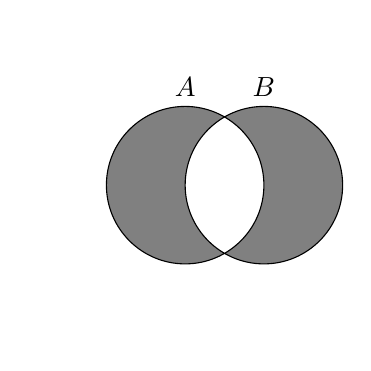
\begin{tikzpicture}[fill=gray]
\scope
\clip (-2,-2) rectangle (2,2)
      (1,0) circle (1);
\fill (0,0) circle (1);
\endscope
\scope
\clip (-2,-2) rectangle (2,2)
      (0,0) circle (1);
\fill (1,0) circle (1);
\endscope
\draw (0,0) circle (1) (0,1)  node [text=black,above] {$A$}
      (1,0) circle (1) (1,1)  node [text=black,above] {$B$};
\end{tikzpicture}
\caption{The shadowed area, a subset of $A$ and $B$, is $(A \cup B) \setminus (A \cap B)$.}
\end{figure}

\bigskip

Unions and intersections have a few crucial properties, which can be further utilized to establish the order of these operations. The following properties are useful to bear in mind while operating with sets:

\begin{itemize}
\item For all $A$ and $B$
\[
A \cup B = B \cup A \qquad \text{and} \qquad A \cap B = B \cap A.
\]
\item  For all $A$, $B$ and $C$
\[
\begin{split}
&(A \cup B) \cup C = A \cup (B \cup C) = A \cup B \cup C \quad \text{and}  \\
&(A \cap B) \cap C = A \cap (B \cap C) = A \cap B \cap C.
\end{split}
\]
\item For all $A$, $B$ and $C$ 
\[
(A \cup B) \cap C = (A \cap C) \cup (B \cap C)\quad \text{and} \quad (A \cap B) \cup C = (A \cup C) \cap (B \cup C).
\]
\item De Morgan's laws.\index{De Morgan's laws} For all $A$ and $B$
\[
(A \cup B)^C = A^C \cap B^C \qquad \text{and} \qquad (A \cap B)^C = A^C \cup B^C. 
\]
De Morgan's laws can be generalized for the intersections and unions consisting of more than two sets, for example for all $A$, $B$ and $C$
\[
(A \cup B \cup C)^C = A^C \cap B^C \cap C^C.
\]
\end{itemize}

\bigskip

In addition, intersections and unions can be defined for infinitely many sets. For example, let $A_1, A_2, \ldots$ be a sequence of sets. The union is now notated as
\[
\bigcup_{j = 1}^{\infty} A_j = \{x : x \in A_j \text{ for some } j\},
\]
and the intersection as 
\[
\bigcap_{j = 1}^{\infty} A_j = \{x : x \in A_j \text{ for all } j\}.
\]

\bigskip

To close the definition of these basic concepts, let's now define the concept of \emph{power set}, which will later on be utilized in defining the sample space of a probability space.


\begin{maar}\label{powerset}\index{Set!Power set}
\emph{Power set.} Let $A$ be an arbitrary set. The \emph{power set} of $A$ is now a set consisting of every subset of $A$:
\[
\mathcal{P}(A) = \{B : B \subseteq A \}.
\]
\end{maar}

To clarify, the definition \ref{powerset} tells us that the power set of $A$ consists of every subset of $A$. According to the definition, empty set $\emptyset$ and the set $A$ itself are also subsets of the set $A$. Thus the power set of an example set $A_1 = \{1, 2, 3\}$ is
\[\mathcal{P}(A_1) = \{\emptyset, \{1\}, \{2\}, \{3\}, \{1,2\}, \{1,3\}, \{2,3\}, \{1,2,3\}\}.
\]

\section{Combinatorics}\label{komb}

\emph{Let us now proceed to basic combinatorics in order to handle sets further.}

Before defining the concept of mathematical probability, let us take a moment to introduce ourselves into the world of combinatorics\footnote{The field of combinatorics researches the number of certain sets, and other questions revolving around counting these sets. Some of the basic concepts of combinatorics have been introduced in the upper secondary level probability courses.}. Let's proceed with an easy example: 

\begin{esim}\label{esim:dice}
\emph{Tossing dice}. Let's toss an ordinary die. In dice tossing\footnote{This can be compared with the intuitive introduction in the introduction chapter.}, the probability can be calculated as a ratio of the number of ''successful'' outcomes and the number of all possible outcomes, the latter being $6$. What is the probability of the outcome being smaller than $5$?

Now we define the ''successful'' outcomes as tosses which end up being smaller than $5$. Now the successful outcomes are 1, 2, 3, and 4, which totals 4 successful outcomes. Thus the probability is $\frac{4}{6}$.
\end{esim}

When the number of possible outcomes is finite and they are all equally likely, the calculation of all existing probabilities are, in principle, as simple as in the previous example. However, when the number of possible  outcomes\index{Outcome} are high, they can not be easily listed separately\footnote{By hand, at least. It also would not be very efficient to print millions of outcomes with a computer program -- the print would hardly be useful for inference.}, and we require some rules to calculate the number of outcomes in the sample space and its subsets. These rules are often referred to as the fiel of combinatorics\footnote{We will be returning to define and examine the concepts of sample spaces and outcomes further in the next chapter.}.

\begin{lause}\label{Basic Principle of Counting} The basic principle of counting.\index{Basic Principle of Counting} Let us make two experiments with $m$ and $n$ different outcomes$(m,n\in\mathbb{N})$. Then, the total number of outcomes of the two experiments is $m\cdot n$.
\end{lause}

\begin{proof}
Let us tag each possible outcome with numbers, $1,$ \ldots, $m$ and $1,$ \ldots, $n$. The proof is to list every possible combination of these outcomes:

\begin{center}
\begin{tabular}{c c c c}
$(1,1)$ & $(1,2)$ & \ldots & $(1, n)$ \\
$(2,1)$ & $(2,2)$ & \ldots & $(2, n)$ \\
\vdots & \vdots & \ldots & \vdots \\
$(m,1)$ & $(m,2)$ & \ldots & $(m, n)$. 
\end{tabular}
\end{center}

Each row has $n$ outcomes and each column has $m$ outcomes. Thus, the total number of outcomes must be $m\cdot n$.
\end{proof}

The basic principle of counting can be expanded into a more general form as the \emph{rule of product}.

\subsection{Rule of Product}\label{ruleofproduct}

In calculating probabilities, it often is handy to know that in how many ways a certain choice can be made, or a certain task can be executed. For example, we could end up choosing a set of dishes: we are asked to make a decision between $2$ different plate types, $3$ different glass types and one set of cutlery available. Together with the first type of plates, we are able to choose three between three types of glasses. Symmetrically, we are able to choose the same amount of glasses together with the first plate -- the total amount of plate-glass combinations is now $6$. Since there is only one option for cutlery, we infer that there must be a total of $6$ different combinations. This train of thought can be expanded into a rule of product, which not coincidentally would give us the same result: $6=2\cdot 3 \cdot 1$.

\begin{lause}\label{thm:ruleofproduct} Rule of Product.\footnote{Also known as the \emph{generalized} or \emph{fundamental basic principle of counting}.} \index{Rule of Product}\index{Fundamental Basic Principle of Counting}

Let us assume that a task can be executed in $k$ subsequent steps, such that the first step has $n_1$ options, the second step has $n_2$ options, and so on, until the last step, which has $n_k$ options. Let us also assume that the amount of options $n_i$ in the step $i$ is not dependant on the choices made in previous steps. Then, the task can be executed in a total of

\[
\prod_{i=1}^k n_i =  n_1 \cdot n_2 \cdot ...  \cdot n_k
\]

different ways.
\begin{proof}
The proof is fairly simple, and it can be done with the help of theorem \ref{Basic Principle of Counting}: we will leave it as an exercise for the reader.
\end{proof}
\end{lause}

Let us now illustrate the theorem with a gambling example, to honour the history of the field of probability.\footnote{The example is based on a game known as \emph{Vakioveikkaus} by the Finnish state-owned gaming monopoly. The author does not, with this example or any subsequent gambling examples, encourage the reader to try gambling services mentioned, and furthermore, the author does not take a stand against or for the current gaming and gambling system in Finland.}

\begin{esim}
We decide to make a gamble, where we bet on $13$ different rows. Each row has three different options (1,X,2), where most often 1 refers to Home winning, X refers to a tie and 2 refers to Visitor winning. Now, due to the theorem \ref{thm:ruleofproduct}, the total number of different rows is
\[
3^{13} = 1594323.
\]
\end{esim}

Utilizing the rule of product, we can also calculate the number of subsets of a given set:

\begin{lause}\label{thm:numberofsubsets}
Number of subsets. A set $E = \{x_1, \dots , x_n\}$ consisting of $n$ elements has $2^n$ different subsets.

\begin{proof}
An arbitrary subset of $E$ can be formulated in $n$ different steps, where in the first step we choose whether the element $x_1$ belongs to the subset, and in the next step we choose whether the next element, $x_2$ belongs to the subset. We repeat such choices until the very last element $x_n$. In each step, there is two possible alternatives: either the element belongs to the subset, or it doesn't. Thus, according to the rule of product, we have a total of $2^n$ possible subsets.
\end{proof}
\end{lause}

\begin{remark}
Theorem \ref{thm:numberofsubsets} gives us the number of elements in the power set $\mathcal{P}(E)$ (see definition \ref{powerset}) of the set $E$. This information will provide itself useful later on.
\end{remark}

\subsection{Rule of Sum}

In addition to the rule of product, there exists another useful calculation rule. \emph{The Rule of Sum}\footnote{Also, in some literature known as the \emph{addition principle}.} can be used in situations, where a task can be executed in a several \textbf{mutually exclusive} steps.

\begin{lause}\label{ruleofsum} Rule of Sum. \index{Rule of Sum}\index{Addition Principle} Let us assume that an experiment can be conducted in $k$ mutually exclusive (disjoint) alternatives. If each alternative $i \in \{1, \dots ,k\}$ has $n_i$ possibilities, then the experiment has a total of 
\[
\sum_{i=1}^k n_i = n_1 + n_2 + \dots n_k
\]
possible results.
\end{lause}

\begin{esim}
A student commutes to a campus. She can either use a direct bus connection with buses 10 and 11, or travel first with bus 20 and then change for buses 21, 22, or 23, or travel first with a metro and then change for buses 30 or 31. The student always picks a commute path, for which means of transportation arrives first, and thus the student picks her commute path randomly. In how many ways can the student get to the campus?

The solution can be presented with the rule of sum as a sum of mutually exclusive commute alternatives. The alternatives are a direct bus connection, commuting with 2 different bus lines and commuting with a metro and a bus. Now we can notate that $n_1 = 2$, $n_2 = 3$ and $n_3 = 2$. Thus the total number of alternatives is $2+3+2 = 7$.
\end{esim}

\subsection{Permutations and Combinations}

The ordering of elements, \emph{permutations}, and subsets, \emph{combinations}, of a set have a central role in the field of probability. Let us illustrate these concepts with following examples.

\begin{esim}
Let us examine a four-element set $A = \{a,b,c,d\}$
\begin{itemize}
\item In how many ways can we order the elements of $A$? The ordering can be split into four steps: first, we select the first element, where we have 4 different alternatives. The second element can be picked from every element but the one we picked first, so there are now 3 alternatives. For the third element, we can pick one of the 2 elements left. Lastly, we have only one element left for the final place. Thus, according to the rule of product, the set $A$ can be ordered in
\[ 
4! = 4 \cdot 3 \cdot 2 \cdot 1 = 24 
\]
different ways.

\item How many different ordered pairs can we pick from the set $A$? In a setting where $A$ is small enough, we are able to list and count every possible pair:
\[
\begin{split}
&(a,b), (a,c), (a,d) \\
&(b,a), (b,c), (b,d) \\
&(c,a), (c,b), (c,d) \\ 
&(d,a), (d,b), (d,c),
\end{split}
\]
that is, 12 pairs. We can also arrive to the same conclusion with the rule of product, since the process of picking ordered pairs can be executed in two steps: first we pick the first element from the four total elements, and then we have three alternatives left for the second member of the pair. Thus, again according to the rule of product, the total number of ordered pairs is
\[
4 \cdot 3 = 12.
\] 

\item How many different subsets of size two -- that is, subsets with 2 elements can we choose from $A$? Again, we are able to list and count all possible alternatives:
\[
\begin{split}
&\{a,b\}, \{a,c\}, \{a,d\} \\
&\{b,c\}, \{b,d\}, \\
&\{c,d\},
\end{split}
\]
from which we total 6 different subsets. We are able to arrive to the same conclusion by noting that every set of two elements can be ordered in two different ways: for example the alternatives in ordering a set $\{a,b\}$ are $(a,b)$ and $(b,a)$. Thus for every subset of 2, we have two different ordered pairs. Before we noted that there exists 12 different ordered pairs, from which we infer that there must be
\[
\frac{12}{2} = 6 
\]
different subsets of two elements.
\end{itemize}
\end{esim}

Let us next add names to the concepts we just learned, and in addition, let us generalize the example to a setting where we examine a set of size $n$.

\begin{maar} \emph{Permutation and Combination}. Let $E = \{x_1 , \dots , x_n\}$ be a set with $n$ elements.
\begin{enumerate}[(i)]
\item A sequence\footnote{Please do note that in \emph{sets} we do not associate each element with any order number, and instead in \emph{sequences}, the order of the elements do matter. We also used notations in a following way: for example, let $\{a,b\}$ be a set, where we denote the set with curly brackets. Now, $\{a,b\}=\{b,a\}$. Instead, if we were examining ordered pairs, denoted with ordinary brackets: $(a,b) \neq (b,a)$.} of length $n$ consisting of the elements of set $E$
\[
(x_{i_1}, x_{i_2} \dots , x_{i_n})
\]
is called the \emph{permutation} of $E$\index{Permutation}.

\item For all $k \in \{1, \dots , n\}$, a sequence which consists of $k$ elements from $E$ (where only element is picked no more than once)
\[
(x_{i_1}, x_{i_2}, \dots ,x_{i_k})
\]
is called the $k$-\emph{permutation} of $E$\index{Permutation!k-Permutation}

\item A $k$-sized subset of $E$ 
\[
\{x_{i_1}, x_{i_2}, \dots , x_{i_k}\}
\]
is called its $k$-\emph{combination}. \index{Combination}\index{k-combination}
\end{enumerate}
\end{maar}

Let us now examine the amount of these permutations and combinations for arbitrary sets.

\begin{lause}
\label{lause:combinations}
The number of permutations and combinations for a given set. Let $E = \{x_1 , \dots , x_n\}$ be a set with $n$ elements.
\begin{enumerate}[(i)]
\item The set $E$ has $n!$
permutations.

\item For all $k \in \{1, \dots , n\}$, the set E $E$ has 
\[
\frac{n!}{(n-k)!}
\] 
$k$-permutations.

\item For all $k \in \{1, \dots , n\}$, the set $E$ has 
\[
\binom{n}{k} = \frac{n!}{k!(n-k)!}
\]
$k$-combinations. 
\end{enumerate}
\end{lause}

\begin{proof} \leavevmode
\begin{enumerate}[(i)]
\item Any permutation of set $E$ can be selected in $n$ steps, such that firstly we pick the first element, secondly the second element, and so on, until the last step with the last element. In the first step, we are able to choose any element of $E$ -- that is, we have $n$ alternatives. Secondly and similarly, we have $n-1$ elements left. Finally, we have are left with only one element. Thus, very similarly as in the illustrative example above, according to the rule of product the permutation can be chosen in 
\[
n \cdot (n-1) \cdot ... \cdot 1 = n!
\]
different ways.

\item Very similarly to (i), but instead we have only $k \in \{1, \dots , n\}$ steps. Thus, in the last step we have as much as $(n-k-+1)$ alternatives left, and the number of different $k$-permutations is
\[
n \cdot (n-1) \cdots (n-k+1) = \frac{(n-1) \cdots (n-k+1) \cdot (n-k) \cdot (n-k-1) \cdots 1}{(n-k) \cdot (n-k-1) \cdots 1} = \frac{n!}{(n-k)!}.
\]

\item Now, let $x$ be the number of the $k$-combinations of $E$. Every $k$-combination is a set of size $k$, and thus according to (i), it can be ordered in $k!$ different ways. Every $k$-permutation of a set can be derived by ordering its $k$-combinations, and thus $E$ has $x \cdot k!$ different $k$-permutations. Matching this newfound information with (ii), we get ourselves an equation, from with $x$ can be solved to get the number of $k$-combinations:
\[
\begin{split}
x \cdot k! &= \frac{n!}{(n-k)!} \\
		 x &= \frac{n!}{k!(n-k)!} = \binom{n}{k}.
\end{split}
\]

\end{enumerate}
\end{proof}

If $n,k \in \N$ are integers, we call  
\[
\binom{n}{k} = \frac{n!}{k!(n-k)!} 
\] 
the \emph{binomial coefficient}.\index{Binomial Coefficient} When $k < 0$, or $k>n$, we define
\[
\binom{n}{k} = 0.
\]

\bigskip

Let us next proceed to examine a few examples on how to calculate the combinations and permutations, and see how the number of types of different problems we are now able to solve expanded gradually.

\begin{esim}\label{esim: poker hand}
Poker hand. Let us pick five cards out of a shuffled standard 52-card deck\footnote{Do remember that in a standard deck of cards, there exist $52$ cards, which are made up by four suits, and each suit consist of cards ranging from $1$ to $13$.}. The order of the cards picked is not currently relevant to us. How many different hands of 5 are there to pick?

Possible combinations of five cards are, for example, 
\[
\{\heartsuit 3, \diamondsuit 3, \heartsuit J, \spadesuit 5, \diamondsuit 9\}
\]
ja
\[
\{\diamondsuit 5, \spadesuit J, \diamondsuit K, \clubsuit 3, \heartsuit A\}.
\]
We note that these can be interpreted as different $5$-combinations out of a $52$-sized deck. Thus the number of different $5$-combinations is, according to the part (iii) of theorem \ref{lause:combinations} a total of 
\[
\binom{52}{5} = \frac{52!}{5!47!}= 2598960.
\] 
\end{esim}

\begin{esim}
The people representing the UN delegations of $11$ countries are sitting across a table in a meeting of UN's Security Council. We regard two sets of positions identical, if we can derive them from each other by rotating the table clockwise or counter-clockwise.
\begin{enumerate}[a)]
\item In how many ways can the seats be ordered?

Let us number each of the delegates with 1, \ldots, 11, and the seats with indexes 1, \ldots, 11 (See the picture below). 
\bigskip

\setlength{\unitlength}{1cm}
\thicklines
\begin{picture}(10,2)
\put(5,1.1){\circle{2}}
\put(5.3, 1.9){1}
\put(5.7, 1.5){2}
\put(5.8, 1.0){3}
\put(5.7, 0.5){4}
\put(5.3, 0.1){5}
\put(4.8, 0){6}
\put(4.3, 0.2){7}
\put(4, 0.6){8}
\put(3.9, 1.1){9}
\put(4, 1.6){10}
\put(4.6, 1.95){11}
\put(5.25, 1.6){\circle*{0.1}}
\put(5.5, 1.4){\circle*{0.1}}
\put(5.55, 1.1){\circle*{0.1}}
\put(5.5, 0.8){\circle*{0.1}}
\put(5.3, 0.6){\circle*{0.1}}
\put(5, 0.5){\circle*{0.1}}
\put(4.7, 0.6){\circle*{0.1}}
\put(4.5, 0.85){\circle*{0.1}}
\put(4.45, 1.15){\circle*{0.1}}
\put(4.55, 1.45){\circle*{0.1}}
\put(4.85, 1.65){\circle*{0.1}}
\put(2.5, 1.75){Pöytä:}
\put(8, 1.75){Edustajat:}
\put(8.3, 1.25){1  2  3  4}
\put(8.4, 0.75){5   6   7   8}
\put(8.3, 0.25){9   10   11}
\end{picture}

Now, according to the part (i) of theorem \ref{lause:combinations}, the eleven delegates can be seated to the eleven seats in $11!$ different ways. This seating, however, includes seatings which can be interpreted identical by rotating the table. To solve out the identicalities, we must divide the answer by the number of possible rotations, and the final answer turns out to be $\frac{11!}{11} = 10! = 3628000$.

\item In how many ways the delegates can be seated in a way where the delegates of England and France are sitting next to each other, but the delegates of USA and Russia are not?

Let us now examine the favorable seatings and situations to derive the seatings from. First, the delegate of England has $11$ possible seats, and from this we deduce that the delegate of France has $2$ possibilities to sit next to the English delegate. In the case where the delegate of USA sits next to France or England (2 alternatives), the delegate of Russia is left with $7$ alternatives since she can not sit next to the delegate of USA. However, if the USA delegate is not sitting next to France or England (7 alternatives), the Russian delegate is left with $6$ possible seats. The rest of the less picky delegates can be seated and ordered in $7!$ different ways. Thus, by combining the rule of product and the rule of sum we arrive with
\[
\begin{split}
&11 \cdot 2 \cdot 2 \cdot 7 \cdot 7! + 11 \cdot 2 \cdot 7 \cdot 6 \cdot 7! \\
=& 11 \cdot 7 \cdot 2 \cdot (2+6) \cdot 7! = 11 \cdot 7 \cdot 2 \cdot 8 \cdot 7! \\ =& 6209280.
\end{split}
\]
Again, the calculations include the identical seats via rotation, and thus the final answer is gained with division:
\[
6209280/11 = 564480.
\]
Alternatively, we could have had ended with identical result with not pinning down the position of the English delegate.
\end{enumerate}
\end{esim}

\bigskip

Let us now stress the fact that binomial coefficient represents a number of how many times are we able to split a $n$-sized set in two, such that the other part has $k$ elements and the other has $n-k$ elements\footnote{Compare this to the example \ref{esim: poker hand}, where the split groups are the picked cards and those not picked.}. As with many mathematical concepts, the binomial coefficient can be generalized to tackle a group which is split into more than two groups. In these kinds of situations we refer to a \emph{multinomial coefficient}.\index{Multinomial Coefficient}

\begin{lause}\label{lause:multinomial coefficient} Multinomial Coefficient.
Let $E = \{x_1, \dots , x_n\}$ be a set of $n$ elements, and let $n_1, \dots, n_k \in \N$ be such that $\sum_{i=1}^k n_i = n$. Now, the set $E$ can be split into $k$ subsets such that, for every $i \in \{1, \dots , k\}$, the  $i$-th subset has $n_i$ elements, in a 
\[
\binom{n}{n_1 n_2 \dots \ n_k} = \frac{n!}{n_1!n_2! \dots n_k!}
\]
different ways.
\end{lause}

\begin{proof}
As before, the selection of subset is quite naturally split into $k$ different steps:
\begin{itemize}
\item To the first subset, we can select any $n_1$ out of $n$, so that according to the part (iii) of \ref{lause:combinations} there are $\binom{n}{n_1}$ alternatives.
\item To the second subset we can select $n_2$ elements from those elements which were not chosen to the first subset: thus the number of alternatives is $\binom{n-n_1}{n_2}$.
\item And, as usual, we carry on the similar train of thought until the $k$-th subset, where we are left with $\binom{n - n_1 - n_2 - \dots - n_{k-1}}{n_k}$ different alternatives.
\end{itemize}

Thus, according to the rule of product, the number of different alternatives is
\[
\begin{split}
&\binom{n}{n_1}\binom{n-n_1}{n_2} \dots \binom{n - n_1 - n_2 - \dots - n_{k-1}}{n_k} \\
=& \frac{n!}{n_1!(n-n_1)!} \cdot \frac{(n-n_1)!}{n_2!(n-n_1 - n_2)!} \cdot \dots \cdot \frac{(n - n_1 - n_2 - \dots - n_{k-1})!}{n_k! (n - \sum_{i=1}^k n_i)!} \\
=&\frac{n!}{n_1!n_2! \dots n_k!} = \binom{n}{n_1 n_2 \dots \ n_k}.
\end{split}
\]
Note that here we utilized the fact that when chaining divisions, the numerators and denominators of the subsequent divisions cancel each other out. The last denominator left turns out to be $(n - \sum_{i=1}^k n_i)!$, and furthermore our assumption states that $\sum_{i=1}^k n_i = n$, which simplifies to $0! = 1$. 
\end{proof}

Let us illustrate the concept of a multinomial coefficient with a simple example.

\begin{esim}
The lecturer has two sisters and one brother\footnote{Please do note, that this may not be a factual piece of information as of Spring 2020. To be frank, the example as a whole is kind of silly. Then again, we overall do require more silly things in our lives, so why not?}. In addition, he has a strawberry, a banana, an apple and an orange. In how many ways the lecturer can divide the fruits to his siblings in a way where the brother gets two fruits, and each of the sisters receive a single fruit?

According to the theorem \ref{lause:multinomial coefficient}, the lecturer can give the fruits away in a total of 
\begin{equation}
\binom{4}{1 1 2} = \frac{4!}{1!1!2!} = \frac{24}{2} = 12
\end{equation}
different ways. To further explain the train of thought, we split the set of four apples into three subsets, such that the first subset is a size of $2$ and the last two subsets consist of only one elements.
\end{esim}

As it turns out, the multinomial coefficient is also a useful tool when we want to calculate that how many different permutations with different elements is possible to create from a \emph{sequence} of a fixed length. The next example illustrates this notion with a sequence of letters\footnote{Also in some literature referred to as \emph{words}.}, of which we want to reorder the letters to form some new words.

\begin{esim}
How many words, or sequences of letters, can we form from the word KOKKOLA\footnote{Kokkola is a town with a population of $50000$, and it is located in the Central Ostrobothnia region.}?

We notice that the word KOKKOLA has 7 letters, which can be ordered in $7!$ different ways. However, the original word includes duplicate letters, and in addition, the orders $K_1 O_1 K_2 K_3 O_2 L A$ and $K_3 O_2 K_1 K_2 O_1 L A$ are different permutations (why?), but form the same word. Thus, to reach the solution, the number of permutations $7!$ must be divided with the number of orders per each letter, from which we get
\[
\frac{n!}{n_K!n_O!n_L!n_A!} = \frac{7!}{3!2!1!1!} = \frac{7!}{3!2!} = 420,
\]
which turns out to be equal to the multinomial coefficient
\begin{equation}
\binom{7}{3 2 1 1} = 420.
\end{equation}
\end{esim}

\section{Exercises}

\begin{enumerate}
\item List the power set $\mathcal{P}(A)$ of the set $A = \{a, b, c, d\}$.
\item Let $A$ and $B$ be sets. express the following claims with the help of different set operations:
\begin{enumerate}[a)]
\item $x$ belongs to both $A$ and $B$
\item $x$ belongs to neither $A$ nor $B$
\item $x$ belongs to at least of one of these sets
\item $x$ belongs to one, and no more than one of these sets
\end{enumerate}
\item In an international alphabet there is 26 letters. The Finnish car licence plate is formed by first picking three letters, and then three numbers.
\begin{enumerate}[a)]
\item What is the total number of licence plates?
\item Let now us assume, that the same letter or number can only occur once in a single plate. What is now the number of possible plates? 
\end{enumerate}
\item Show $\binom{n}{k} = \binom{n}{n-k}$, and afterwards explain the result intuitively.
\item (Ross Exercise 1.11) From 8 different locks and the 8 keys fitting to these locks, we want to pick 6 items, such that among the picked items, there is no key that would fit into any of the picked locks.
\begin{enumerate}[a)]
\item How many sets of 6 items are we able to select?
\item What if we wanted to limit our options to only 3 keys and 3 locks?
\end{enumerate}
\item A student participates in an examination, where she has to answer to 7 questions out of 10. Each question is a multiple choice assignment, where there are three alternatives. In how many ways you can turn in the exam?
\item Show that $\binom{n+m}{k} = \binom{n}{0} \binom{m}{k}  + \binom{n}{1} \binom{m}{k-1}  + \ldots + \binom{n}{k} \binom{m}{0}$. (Hint: Think of a set consisting of $n$ adults and $m$ children. How many sets of size $k$ are we able to organize?)
\item A certain alphabet set has only 7 letters. How many sequences (words) of 
\begin{enumerate}[a)]
\item exactly ten letters or 
\item at most ten letters  
\end{enumerate}
are we able to form? 
\item A junior football team has 15 players. In the opening set of players, there must be 2 attackers, 3 players in the middle and 3 defenders, and in addition a goalie. In how many ways can we select the opening set of players? (HINT: Multinomial coefficient.)
\item How many different sequences of 11 letters can we form from the word M, I, S, S, I, S, S, I, P, P, I? 
\item (Ross Exercise 1.16) How many of the $4$-element subsets of \{1,2, \ldots, 20\} include some of the elements 1,2,3,4,5?
\item In a certain high-rise apartment building, there lives 2 families with a parent and a child, one family with a single parent and two children, 5 families with two parents and one child, 6 families with two parents and two children. In how many ways we can select a parent and a child from a same family?
\end{enumerate}

\bigskip

%%%%%%%%%%%%%%%%%%%%%%%%%%%%%%%%%%%%%%%%%%%%%%%%%%%%%%%%%%%%%%%%%%%%%%%%%%%%%%

\chapter{Mathematical Approach to Probability}\label{math.prob}

\section{Classical Probability}\label{classprob}

\emph{This section is to tie the previous illustrative examples with the classical definition of probability, and thus combine the rules of combinatorics into calculating probabilities formally.}

In this course we examine and handle probability as a mathematical concept, and its purpose to model randomness in the real-world phenomena. Often we refer to \emph{random experiment}, which we want to model.\index{Random experiment} In the most simple occasions, the number of possible outcomes of this experiment is finite and they are all equally likely. In such cases, we have a \emph{symmetric} and \emph{finite} probability space, as in example \ref{esim:dice}.

More examples of such random experiment can be either tossing a coin, picking a poker hand from a deck, lottery or a spin of a roulette wheel. As in the previous chapter \ref{intro} was mentioned, this historically earliest way to model probabilities was innovated on gambling.

In cases, where every outcome are symmetric, the probability of an event is calculated as a ratio of the number of favourable or ''successful'' outcomes, and the number of all possible outcomes. This is often referred to as the classical definition of probability.

We have already calculated simple examples without explicitly defining the concepts of sample space or classical probability. Finally, let us define these concepts and then carry on with some examples.

\begin{maar}\label{samplespace} \emph{Sample Space.} Let $\Omega$ be the set of all possible outcomes in a random experiment. We refer to it as the \emph{sample space}, \index{Sample Space} and its elements as $\omega \in \Omega$ \emph{outcomes}. \index{Outcome}
\end{maar}

\begin{maar}\label{maar:outcome}
In the case of finite sample space $\Omega = \{\omega_1, \dots, \omega_n\}$ we refer all subsets $A \subseteq \Omega$ of the sample space as \emph{events}. \index{Event}
We denote the set of all possible events as $\F$. In the case of a finite sample space, this is the set of all possible subsets of $\Omega$\footnote{Note that this allows to use the power set of the sample space as the set of all possible events! Also note, that this is something we can not do when the sample space is finite.}.
\end{maar}

\begin{maar}
\label{maar:classprob} \index{Probability!classical} \index{Classical Definition of  Probability}
\emph{Classical Definition of Probability.} Let $A\subseteq \Omega$ be an event of a finite and symmetric sample space $\Omega$. Now, the probability of event $A$ is 
\[
P(A) = \frac{|A|}{n},
\]
where $|A|$ stands for the number of elements in $A$ and $n := |\Omega|$ is the number of elements in the sample space.  
\end{maar}

To clarify, let us repeat that in the classical definition of probability, all outcomes are equally likely, since it holds that
\[
P(\{\omega\}) = \frac{|\{\omega\}|}{n} = \frac{1}{n} \quad \text{kaikille} \,\, \omega \in \Omega.
\]

Let us now examine the concepts of sample space, outcome, and the classical definition of probability in practice!

\begin{esim} Let us toss a coin once. Now the outcomes are $\omega_1 = $ head and $\omega_2 = $  tails. Thus the sample space 
\[
\Omega = \{\mathrm{head, tails} \},
\]
includes $n=2$ outcomes, and the set of all possible events is
\[
\F = \{\emptyset,  \{\mathrm{head} \}, \{\mathrm{tails}\} , \{\mathrm{head} ,\, \mathrm{tails} \}  \}. 
\]
The probabilities for these events are: 
\[
\begin{split}
&P(\emptyset) = 0 \quad \text{(no head or tails)} \\
&P(\{\mathrm{head}\}) = \frac{1}{n} = \frac{1}{2} \\
&P(\{\mathrm{tails}\}) = \frac{1}{n} = \frac{1}{2} \\
&P(\{\mathrm{head, \, tails}\}) = P(\Omega) = 1 \quad \text{(head or tails)}. 
\end{split}
\]
\end{esim}

\begin{remark}
\label{huom:brackets}
To simplify the notation, we usually leave the second pair of brackets out -- that is, the probability of event $\{ \omega_1, \omega_2\}$ can be simplified as
\[
P(\{ \omega_1, \omega_2\}) = P\{ \omega_1, \omega_2\}, 
\]
or as
\[
P(\{ \omega_1, \omega_2\}) = P(\omega_1, \omega_2). 
\]
In this material, we will use the latter notation, and thus the probability in the last example for the event $\{\mathrm{head, \, tails}\}$ (the result is head or tails) can be written more shortly as 
\[
P(\mathrm{head, \, tails}).
\]
\end{remark}

\begin{esim}
Picking one card from the standard 52-card deck. Let us assume, that the deck is shuffled. The outcomes can now be, for example $\spadesuit 2$, $\clubsuit 7$ and $\heartsuit J$. Furthermore, the sample space is now
\[
\Omega = \{(x,y) \,|\, x \in \{\clubsuit, \spadesuit, \diamondsuit, \heartsuit\}, y \in \{2,3, \dots, 10, J, Q, K, A\}\}.
\]
The sample space has $n=52$ elements, which could be, in principle, still listed. However, do note that there exists $2^{52}$ different events\footnote{As in the definition \ref{maar:outcome}, the set of all possible events is now the sample power set of the sample space: each outcome can be thought as a member or a non-member of each event, and similarly as in \ref{thm:numberofsubsets}, the number of all possible events is now $2^{52}$.}, so we can reasonably argue that it would not be possible to list every single one of them. Let us instead examine few example events. An event can be, for example $A:$ ''a card is of a black suit'':
\[
A = \{(x,y) \in \Omega \,|\, x \in \{\spadesuit, \clubsuit \}\},
\]
and $B:$ ''a card is a diamond and ja smaller than 5'':
\[
B = \{(x,y) \in \Omega \,|\, x \in \{\diamondsuit\} \,\, \text{ja} \,\, y \in \{2,3,4\} \}.
\]
The probability for these events can be directly calculated with the classical definition of probability:
\[
P(A) = \frac{|A|}{n} = \frac{26}{52} = \frac{1}{2}
\] 
and
\[
P(B) = \frac{|B|}{n} = \frac{3}{52}.
\]
\end{esim}

\begin{esim}\label{esim: two dice} Tossing two six-sided dices. The outcomes are the ordered pairs
\[
(1,1), (1,2), \dots , (6,5), (6,6),
\]
that is, $\Omega = E \times E$, $E = \{1,2, \dots , 6\}$.  

Now the number of unique events is $2^{36}$. Let us denote the event ''The sum of two dices is over 9'' as $A$. Now we can write $A$ as 
\[
\begin{split}
A 	&= \{ (x,y) \in \Omega \,|\, x+y > 9\} \\
	&= \{ (4,6), (5,5), (5,6), (6,4),(6,5), (6,6) \}.
\end{split}
\]
Now, according to the classical definition of probability
\[
P(A) = \frac{|A|}{n} = \frac{6}{36} = \frac{1}{6}.
\]
Let us now denote the event ''both dices are smaller than three'' as $B$. Now $B$ can be written as
\[
\begin{split}
B 	&= \{ (x,y) \in \Omega \,|\, x < 3 \,\,\text{and} \,\, y < 3\} \\
	&= \{ (1,1), (1,2), (2,1), (2,2) \}.
\end{split}
\]
Again, borrowing the power of the classical definition, we get
\[
P(B) = \frac{|B|}{n} = \frac{4}{36} = \frac{1}{9}.
\]
\end{esim}

\begin{esim}
Let us take a moment to reminisce combinations and the example \ref{esim: poker hand}, the poker hand. In such occasion, it may be wise to think the sample space $\Omega$ as every subset of size $5$ from the 52-card deck. As in the example, we remember that the number of $5$-combinations -- that is, the number of different hands, is a total of $\binom{52}{5} = 2598960$.

Thus the probability of any single five-card combination, for example a royal flush of hearts, is
\[
P\{\heartsuit 10, \heartsuit J, \heartsuit Q, \heartsuit K, \heartsuit A\} = \frac{1}{\binom{52}{5}} = \frac{1}{2598960} \approx 3.85 \cdot 10^{-7}. 
\]

Let us next calculate a probability for the event $A:$ ''pick a hand with four aces''. This special kind of $5-$combination must include at least the cards $\heartsuit A,\diamondsuit A, \clubsuit A$ and $\spadesuit A$. Do note, that the last card can be any of the remaining 48 cards -- now the event $A$ includes 48 outcomes (different poker hands) from the sample space, and the probability for $A$ is now
\[
P(A) = \frac{48}{\binom{52}{5}} \approx 	1.85 \cdot 10^{-5}.
\]
\end{esim}

\begin{esim}
\label{esim:aces}
More practice would not hurt! Let us calculate probabilities for events $B:$ ''pick a hand with exactly three aces'' and $C:$ ''pick a hand with no less than three aces''. When calculating probabilities for such events, it may be wise to pay attention and not calculate each individual hand multiple times.

Let us first calculate the number of hands with exactly three aces. We can split the picking process into two steps: first, let us pick three aces, and afterwards pick the rest. Three aces can be picked in four different ways:
\[
\begin{split}
&\{\heartsuit A,\diamondsuit A, \clubsuit A\}, \\
&\{\heartsuit A,\diamondsuit A, \spadesuit A\}, \\
&\{\heartsuit A,\spadesuit A, \clubsuit A\}, 
\end{split}
\]
or
\[
\{\spadesuit A,\diamondsuit A, \clubsuit A\}.
\]
In the second step we pick the 2 cards that are left. There are 48 possible alternatives, since three of the aces are already in hand and the last ace is not favourable for us, since the hand would have more than  3 aces (remember, we wanted the exact amount of 3). According to the part (iii) of the theorem \ref{lause:combinations}, we can pick sets of two cards, 2-combinations, from the 48 card set in $\binom{48}{2} = 1128$ different ways. Furthermore, according to the rule of product, the number of hands including exactly three aces, is $4 \cdot 1128 = 4512$. Finally, the desired probability turns out to be 
\[
P(B) = \frac{4512}{\binom{52}{5}} \approx 0.001736.
\]

The number of hands with no less than three aces can be acquired with combining the number of hands with exactly three aces with the number of hands with exactly four aces: the numbers sum up to the total of $4512 + 48 = 4560$ hands. Thus, the probability of getting no less than three aces is
\[
P(C) = \frac{4560}{\binom{52}{5}} \approx 0.001755.
\] 
\end{esim}

\subsection{Sampling}\label{sampling} \index{Sampling}

In many occasions, when conducting a statistical research, we want to examine properties of some statistical populations. Questions of interest might be, for example, that what is the percentage of Finns to support Finland joining NATO, or what is the percentage of undergrown fishes in a lake. Asking every five and a half million of Finns whether they like the idea of joining NATO, or fishing every fish in the lake, is practically impossible, which is why questions such as these are examined with sampling -- that is, selecting a subset of the population to estimate the characteristics or properties of the whole population. We call this subset a sample, and most often the sample is much smaller than the size of the whole population. Sampling can be done with or without replacement. In the former case, an individual can be sampled more than once, and in the latter case an individual can be sampled only once. Let us now shrink the ball park, and examine a ball example!

\begin{esim}
\label{esim:balls}
Let us have a box. In the box there are 8 balls, of which 5 are white and the rest, $8-5=3$, are black. The box can now be modelled as a set
\[
E = \{w_1, w_2, w_3, w_4, w_5, b_1, b_2, b_3\},
\]
where with $w$ we denote a white ball, and with $b$ we denote a black ball.

\begin{enumerate}[(i)]
\item \textbf{Sampling without replacement.} 
Let us pick up four balls randomly, without replacing the balls back to the box. What is the probability for the event $A_2$ = ''pick up exactly two white balls''?

It is wise to pick every 4-combination of the set of 8 balls as the sample space: without replacement, the order of the balls is not relevant to the event at hand. Outcomes from the sample space are, for example,
\[
\{w_3, w_4, b_1, b_3\}
\]
and
\[
\{w_1, w_2, w_4, b_1\}.
\]

According to the part (iii) of theorem \ref{lause:combinations}, there are a total of $\binom{8}{4}$ outcomes. Of these, favourable to the event $A_2$ are those with two white balls and 2 black balls -- that is, for example,
\[
\{w_3, w_4, b_1, b_3\}
\]
ja
\[
\{w_1, w_4, b_1, b_2\}.
\]

According to the part (iii) of theorem \ref{lause:combinations}, the white balls can be picked in $\binom{5}{2}$ different ways and the black balls can be picked in $\binom{3}{2}$ different ways. Thus the number of possible combinations with exactly two white balls, is according to the rule of product $\binom{5}{2}\binom{3}{2}$. Finally, the probability of picking exactly 2 white balls is

\[
P(A_2) =  \frac{\binom{5}{2}\binom{3}{2}}{\binom{8}{4}} = \frac{10 \cdot 3}{70} = \frac{3}{7} \approx 0.4286.
\]

\item \textbf{Sampling with replacement.} 
Let us randomly pick 4 balls from the box, with replacing each ball back to the box between the picks. What is the probability for event $A_2$ = ''pick up exactly two white balls''?

Now, as opposed to the previous example, the order of the picks matter, and thus it would be wise to select every sequences of 4, which are possible to pick from the set of eight balls and where a single ball can appear more than once, as the sample set $\Omega$. Examples of the outcomes would now be:
\[
(b_3, b_3, b_1, b_3)
\]
ja
\[
(w_3, w_2, w_3, b_2).
\]

According to the rule of product (section \ref{ruleofsum}) there are $8^4$ of these sequences. 

Let us now infer, how many of these sequences have exactly two white balls. First let's examine, in how many ways can we order 4 balls, such that 2 of them are white and 2 of them are black, as sequences. Such sequences could, for example, look like
\[
(b, b, w, w)
\]
and
\[
(w, b, w, b).
\]
Again, according to the part (iii) of theorem  \ref{lause:combinations}, there are $\binom{4}{2}$ permutations satisfying these conditions. Furthermore, we can pick the white and black balls or these permutations in multiple ways. For example, the permutation $(b, b, w, w)$ is satisfied by

\[
(b_2, b_2, w_5, w_3)
\]
and
\[
(b_3, b_1, w_1, w_3).
\]

According to the rule of product, the white balls can be selected in $5^2$ different ways, while the black balls can be selected in $3^2$ different ways.

Furthermore, again according to the rule of product, the number of different sequences of 4 balls, of which 2 are white, is $\binom{4}{2} \cdot 5^2 \cdot 3^2$. Finally, the probability of picking exactly 2 white balls is
\[
P(A_2) = \frac{\binom{4}{2} \cdot 5^2 \cdot 3^2}{8^4} = \frac{1350}{4096} \approx 0.3296.
\]

\end{enumerate}
\end{esim}

\bigskip

Let us now generalize this setting. Let  $E = A \cup B$ be a set with $N$ elements, where $A = \{a_1, \dots, a_K\}$ and $B =\{b_1,\dots,  b_{N-K}\}$. For example and illustrative purposes, $E$ can be a set of $K$ white balls and $N-K$ black balls in a box. Thus, the previous example is generalized in a following way:

\begin{lause}
\label{lause:sampling} Sampling without and with replacement. Let $n\in \{1, \dots , N\}$ and $k \in \{0, \dots , n\}$. 

\begin{enumerate}[(i)]
\item \index{Sampling!without replacement}
Let us pick a sample of $n$ from the set $E$, randomly without replacement. The probability for the event $A_k:$ ''in the sample there are exactly $k$ elements of $A$'' is

\[
P(A_k) = \frac{\binom{K}{k}\binom{N-K}{n-k}}{\binom{N}{n}}.
\]

\item \index{Sampling!with replacement}
Let us pick a sample on $n$ from the set $E$, randomly with replacement. Now the probability for event $A_k:$ ''in the sample there are exactly $k$ elements of $A$'' is

\[
P(A_k) = \binom{n}{k} \frac{K^k(N-K)^{(n-k)}}{N^n}.
\]

\end{enumerate} 
\end{lause}

\begin{proof}
Exactly as in the previous example \ref{esim:balls}.
\end{proof}

We can model a picking of a poker hand from a 52-card standard deck as a sampling without replacement. Thus, the result from example \ref{esim:aces} with exactly three aces is derived directly from the previous theorem, when we choose $N=52$, $K=4$, $n=5$ and $k=3$:
\[
P(B) = \frac{\binom{K}{k}\binom{N-K}{n-k}}{\binom{K}{n}} = \frac{\binom{4}{3}\binom{48}{2}}{\binom{52}{5}} \approx 0.001736.
\]

If, on the other hand, we would pick 5 cards, such that the picked card was always returned into the deck and shuffled, we would model the situation as sampling with replacement. In such setting, the probability for exactly three aces is, when notating such event with $D$:

\[
P(D) = \binom{n}{k} \frac{K^k(N-K)^{(n-k)}}{N^n} = \binom{5}{3} \frac{4^3 \cdot 48^{2}}{52^5} \approx 0.003878.
\]

\bigskip

\begin{remark}
It is important to note that the selection of the sample space is always arbitrary, and the same random experiment can be modelled with multiple different sample spaces. Often, as is with the examples of this section, the sample set can be the obvious one. However, there are multiple alternatives: for example, if we were interested only in the sum of two dices, we could use the set of summed totals as the sample space: 

\[
\Omega_1 = \{2, \dots , 12\}.
\]

With this newlyfound sample space, we could represent the event $A$ of the example \ref{esim: two dice} (sum of two dice over 9) as 
\[
A = \{\omega \in \Omega_1 \,|\,  \omega > 9\} = \{10,11,12\}.
\]

However, we would not be able to represent the event $B$ (both dices less than 3) with the sample space of $\Omega_1$. Thus, the sample space needs to be so rich, that every events we are interested in in any given experiment, could be represented as its subsets.

Moreover, when considering event $A$, we can not apply the classical definition of probability with the sample set $\Omega_1$, since the probabilities are not equal and thus the setting is not symmetric.\end{remark}

This remark hints to the possibility that the classical definition of probability is not always the best choice. Let us imagine a situation, where we toss a coin until we get tails as a result. What is the sample space in a such setting? You would soon notice, that $|\Omega| = n =  \infty$. Why? This severely limits the possibilities of the classical definition, and it also is the reason why we would need more definitions for probability. Examples of such definitions would be, for example the frequentist and subjective definitions of probablities. 

%\footnote{Katso kappale \ref{tulkinnasta}}.

\section{Probability Axioms}\label{axioms}

\emph{In this section, we define the probability with the axioms of probability. It sounds self-justified, and in addition, provides us a more general understanding for the concept of probability.}

If the sample space $\Omega$ is not symmetric -- that is, we have no ground to claim that the outcomes would be equally likely, the classical definition \ref{maar:classprob} can not be used to model the uncertainty in a random experiment. Examples of such settings could be throwing five darts, where the sample space can be set as $\Omega = \{0,1,2, \dots, 10\}^5$, a football match, where a natural sample space would be $\N^2$, or a result for a javelin throw, where the sample space can be set as $\Omega = (0, \infty)$.

The two latter examples are anomalies compared to the previous examples, in a way that the sample spaces introduced are infinite. In addition, in the last example sample space is uncountable\footnote{The concept of uncountable sets is often used in the field of measure theory. To introduce the concept briefly, we call a set \emph{countable}, if we can list all its elements. This could mean, for example, the set of natural numbers \{1,2,3, \ldots\}. We define an uncountable set as a set which is not countable: examples of such sets could be the numbers of real axis, or the real numbers between the interval $[0,1]$: we could not list all the numbers of these sets, not even in theory.} infinite (at least in theory).

This train of thought calls for a more general definition, compared to the classical one \ref{maar:classprob} -- on other hand we need it for the non-symmetric random experiments, and on the other hand we need it to handle larger sample spaces.

We then define a set of certain crucial properties for probability, which we call the \emph{axioms of probability.}. Together, the axioms define probability as a set mapping from the set of events $\mathcal{F}$  to the interval $[0,1]$. 

As hinted before, when the sample space $\Omega$ is finite or, at most, countably infinite, we can always choose the power set $\mathcal{P}(\Omega)$ of the sample space to act as the set of all possible events $\F$. In the unfortunate case\footnote{As some of you will realize later on, this is actually the case for a majority of interesting random experiments.} where the sample space is uncountably infinite, we require that the set of all possible events is a so-called \emph{$\sigma$-algebra}.

\bigskip

\begin{maar} 
\emph{$\sigma$-algebra}. A collection $\F$ of the subsets of the sample space $\Omega$ is a \emph{$\sigma$-algebra}\index{Sigma-algebra}, if 
\begin{enumerate}
\item $\Omega \in \F$
\item $A \in \F \Rightarrow A^c \in \F$
\item $A_i \in \F \Rightarrow \bigcup_{i=1}^\infty A_i \in \F$.
\end{enumerate}
\end{maar}

\bigskip

In the most practical sense in the framework of probability, the conditions of $\sigma$-algebra mean that we can only examine a collection of events, which is ''smooth'' enough. The following theorem will help to handle the collection $\F$:

\begin{lause}
Properties of $\sigma$-algebra. Let $\mathcal{F}$ be a  $\sigma$-algebra. Then
\begin{enumerate}[(i)]
\item $\emptyset \in \mathcal{F}$,
\item If $A,B \in \mathcal{F}$, then $A\cup B, A\cap B, A\setminus B \in\mathcal{F}$,
\item $A_i \in \mathcal{F} \Rightarrow \bigcap_{i=1}^\infty \in \mathcal{F}$.
\end{enumerate}
\end{lause}

\begin{proof}
Left as an exercise. Idea behind the proof: part $(i)$ follows from the fact that $\Omega^c = \emptyset$. Part  $(ii)$ is proven by applying the part 3 of the definition, and finally the part $(iii)$ is proven with the help of de Morgan's laws.
\end{proof}

\bigskip

Before the firepower provided us by the measure theory, further examination of $\sigma$-algebra might not be fruitful in the context of this course. Thus we leave the further examination of $\sigma$-algebra, and define the probability\footnote{Also known as the \emph{probability measure} or \emph{probability mapping}.} with the help of the \emph{axioms of probability}\footnote{The axioms were first introduced in Kolmogorov's Foundations of the Theory of Probability (1933)}:

\begin{maar}
\label{maar:prob}
\emph{Probability axioms.}\index{Probability Axioms}\index{Axioms of Probability}\index{Probability Measure} Let $\Omega$ be a sample space and $\sigma$-algebra $\F$ the set of all possible events. A mapping $P:\mathcal{F} \rightarrow \R$ is a \emph{probability}, if
\begin{enumerate}[(PROB1)]
\item $P(A) \geq 0$ for every event $A \in \F$,
\item $P(\Omega) = 1$,
\item For all events $A_1, A_2, \ldots \in \F$  
\[
P\left(\bigcup_{i=1}^\infty A_i\right) = \sum_{i=1}^\infty P(A_i), 
\]
when the events are mutually exclusive, that is, when $A_i \cap A_j = \emptyset$ for all $i \neq j$. 
\end{enumerate} 

\bigskip
The first axiom (PROB1) demands that the probability for each event has to be non-negative, that is, no less than zero. The second axiom (PROB2) in turn demands that the probability for sample space $\Omega$ has to be $1$ -- that is, with each random experiment we have at least some outcome\footnote{This characteristic is often referred to as outcomes being  \emph{collectively exhaustive}.}. The third axiom (PROB3) lastly demands that the probability of a countable union of each disjoint set must equal the sum of the probabilities of these disjoint events. In other words, the probability for an event where at least one of these disjoint events $A_i$ occur is the sum of the individual probabilities $P(A_i)$. This property is known as the \emph{additivity of probability.} 
\end{maar}

After defining the concept of probability, we are finally able to construct a \emph{probability space}\footnote{Also known as a \emph{probability triplet}.}, which is the foundation for modeling random events.

\begin{maar}
\emph{Probability Space.}\index{Probability Space} The triplet $(\Omega, \F, P)$, where $\Omega$ is the sample space, $\sigma$-algebra $\F$ the set of all possible events within the sample space, and $P: \F \rightarrow \R$ a probability, is denoted as a \emph{probability space}.
\end{maar}

Let us next introduce some special cases for our probability space, which are \emph{discrete probability space}, \emph{finite probability space} and the \emph{symmetric probability space}, of which the last one was examined shortly together with the introduction of classical definition of probability.

\begin{maar}
\emph{Discrete Probability Space.}\index{Probability Space!Discrete} If the sample space $\Omega$ is finite $\Omega = \{\omega_1, \dots , \omega_n\}$ or countably infinite $\Omega = \{\omega_1, \omega_2, \dots \}$,
it is always possible to choose the set of every subset of the sample space $\mathcal{P}(\Omega)$ as the set of examined events $\F$, then the probability space $(\Omega, \mathcal{P}(\Omega), P)$ is known as the discrete probability space.

Since the set of possible events $\F$ can always be chosen as the power set of the sample space, we can shorten the notation as $(\Omega, P)$.
\end{maar}

\bigskip

\begin{maar}
\emph{Finite Probability Space.}\index{Probability Space!Finite} Let $(\Omega, P)$ be a discrete probability space. If its sample space $\Omega$ is finite -- that is, if $\Omega = \{\omega_1, \dots , \omega_n\}$ for some $n \in \{1,2, \dots\}$, then we call the probability space a finite probability space.
\end{maar}

Let us next show one basic property of a discrete probability space: in a discrete probability space, we are able to calculate a unique probability for every event as the sums of probabilities of the different outcomes.

\begin{lause}
\label{lause:discrete_prob}
Let $\Omega$ be either finite $\Omega =\{\omega_1, \dots, \omega_n\}$ or infinite $\Omega = \{\omega_1, \omega_2, \dots\}$ sample space of a discrete probability space, and define respectively numbers $p_1, \dots , p_n$ or $p_1, p_2, \ldots \geq 0$ such that\footnote{To simplify notation, in this theorem we are going to use the exact sum notation $\sum_{i=1}^\infty p_i$ for both finite and infinite sample spaces, and clear the following ambiguity by setting $p_i=0$ for every $i>n$ in the finite case. The reason for this is the simple algebraic property that if $p_i=0$ for every $i>n$, then $\sum_{i=1}^\infty p_i = \sum_{i=1}^n p_i$.} $\sum_{i=1}^\infty p_i = 1$. Now there exists a unique probability -- that is, a set mapping $P:\mathcal{P}(\Omega)\rightarrow \R$ which satisfies axioms (PROB1)--(PROB3) -- for which 
\begin{equation}
\label{eq:discrete_prob}
P(\omega_i) = p_i \quad \text{for all} \quad i \in \{1,2, \dots \}.
\end{equation}

\end{lause}

\begin{proof}
To proof this theorem, we need to show that there exists at least one probability which satisfies \ref{eq:discrete_prob}. We notate this step as ''$\Rightarrow$''. In addition, we need to show that this probability is indeed unique, and we refer this step as ''$\leftarrow$''. Let's proceed!

''$\Rightarrow$'': We have to show that given the assumptions in the theorem, there exists a set mapping $P$, which satisfies the probability axioms and the equation \ref{eq:discrete_prob}. 

For every $A \in \mathcal{P}(\Omega)$, let us define the value of $P:\mathcal{P}(\Omega) \rightarrow \R$ as

\begin{equation}
\label{eq:discrete_prob2}
P(A)  := \sum_{\omega_i \in A} p_i.
\end{equation}

\bigskip

From this definition of $P$, it directly follows that $P$ satisfies the condition \ref{eq:discrete_prob}. In addition, we need to check that this newly defined $P$ satisfies the axioms of probability:

\begin{enumerate}[(PROB1)]
\item According to the definition \ref{eq:discrete_prob2} of $P$, for the event $A \in \mathcal{P}(\Omega)$ holds that 
\[
P(A) = \sum_{\omega_i \in A} p_i \geq 0,
\]
where the non-negativity follows from our assumption $p_i \geq 0$, which holds for every $i \in \{1,2, \dots\}$.

\item Again, combining the definition \ref{eq:discrete_prob2} and an assumption from the theorem, we see that for the sample space $\Omega$
\[
P(\Omega) = \sum_{\omega_i \in \Omega} p_i = \sum_{i=1}^\infty p_i = 1.
\]

\item Finally, let $A_1, A_2, \dots \in \mathcal{P}(\Omega)$ be a sequence of mutually exclusive events. Now, in addition, the union of the events $A := \bigcup_{j=1}^\infty A_j \in \mathcal{P}(\Omega)$ can be presented as a countable union of the elements in the sample space: $A = \bigcup_{\omega_i \in A} \{\omega_i\}$. Thus, a property called full additivity ensues:

\[
\begin{split}
&P\left(\bigcup_{j=1}^\infty A_j \right) 
= P\left(\bigcup_{j=1}^\infty \bigcup_{\omega_i \in A_j} \{\omega_i\} \right) 
= P\left(\bigcup_{\omega_i \in A} \{\omega_i\} \right) = P(A) \\
&\overset{(\ref{eq:discrete_prob2})}{=} \sum_{\omega_i \in A} p_i
= \sum_{j=1}^\infty \sum_{\omega_i \in A_j} p_i
\overset{(\ref{eq:discrete_prob2})}{=} \sum_{j=1}^\infty P(A_j).
\end{split}
\]
To make sure that the second last equality sign truly represents an equality, we utilized the assumption of mutually exclusiveness of $A_1, A_2, \dots$.
\end{enumerate}

With these steps, we are always able to find a probability $P$ satisfying the condition \ref{eq:discrete_prob}. Let us now proceed to the second step, where we show that the probability is indeed unique -- that is, if an arbitrary probability $P^*$ satisfies the condition \ref{eq:discrete_prob}, then it must follow that $P^* = P$, and thus $P^*(A) = P(A)$ holds for every event $A \in \mathcal{P}(\Omega)$.

\bigskip

''$\Leftarrow$'': Let $P^*$ be a probability -- that is, a set mapping $P^*:\mathcal{P}(\Omega) \rightarrow \R$ satisfying the axioms (PROB1)--(PROB3), for which the equation \ref{eq:discrete_prob} holds. Let us proceed by showing that for every set $A \in \mathcal{P}(\Omega)$, the equation \ref{eq:discrete_prob2} holds: 
\[
P^*(A) = \sum_{\omega_i \in A} p_i,
\]
from which directly follows $P^*=P$.

\bigskip

We are able to show this by contradiction, so let us make a contradictory claim: that there would exist a set $A \in \mathcal{P}(\Omega)$, such that
 \[
P^*(A) \neq \sum_{\omega_i \in A} p_i.
\]

From this contradictory it follows that for disjoint sets\footnote{You should see that both the union $\bigcup_{\omega_i \in A} \{\omega_i\}$ and the sum $\sum_{\omega_i \in A} P^*(\omega_i)$ are countable operations -- if $A$ is finite, we will select that the ''excess'' sets are empty sets $\emptyset$.} $\{\omega_i\} \in A$ hold that
\[
P^*\left(\bigcup_{\omega_i \in A} \{\omega_i\} \right) = P^*(A) \neq \sum_{\omega_i \in A} p_i \overset{\ref{eq:discrete_prob}}{=} \sum_{\omega_i \in A} P^*(\omega_i).
\]

The difference of the left-hand side and the right-hand side is contradicting the full additivity assumption of $P^*$. Thus the contradictory claim leads to a contradiction, and it can not hold. Instead, it must be that $P^* = P$. 
\end{proof}

Let us now showcase the concept of a symmetrical probability space as an example, where we utilize the theorem \ref{lause:discrete_prob} of a discrete probability space to calculate probabilities for symmetric probability spaces\footnote{Do note, that this is the result that we utilized before when calculating illustrative examples for probabilities.}.

\begin{esim}
Symmetric Probability Space. Let $\Omega = \{\omega_1, \dots, \omega_n\}$ be the sample space, and let us set
\[
P(\omega_i) = p_i = \frac{1}{n} \quad \text{kaikille} \quad i \in \{1, \dots ,n\}.
\]
Now, from the theorem \ref{lause:discrete_prob} it follows\footnote{Do note, that $\sum_{i=1}^n p_i = 1$.} that $P$ defines a unique probability for events $A \in \mathcal{P}(\Omega)$, such that 
\begin{equation}
\label{eq:symmetrinen_tn}
P(A) = \sum_{\omega_i \in A} p_i = \frac{|A|}{n}. 
\end{equation}

Such probability space $(\Omega, P)$, where the probabilities of all outcomes are equal, is called a \emph{symmetric} probability space.\index{Probability Space!Symmetric}

It is important to note that by defining $P$ in such manner, the $P$ is equal with the classical definition of probability \ref{maar:classprob}. From this observation follows that the classical definition is a special case of the generalized definition of probability \ref{maar:prob}.
\end{esim}

\bigskip

Every example we have introduced so far in this material, such as a coin toss, dice toss, poker hand and picking balls from a box have been \emph{modelled} with the help of symmetric probability space. Let us next introduce an example of asymmetric discrete probability space in both finite and infinite\footnote{It can be shown, with the help of the axioms of probability, that no infinite discrete probability space can be symmetric.} sample spaces. 

\begin{esim}
\label{esim:passthepig1}
Pass the Pig. In the famous Pass the Pig game, players toss a ''die'' which is shaped like a pig. The players receive points depending on the position with which the pig lands after a toss. The points and frequencies\footnote{The frequencies are gathered by observing a flat ground and a tossing machine with a sample size of $n=11954$. Source: \url{https://en.wikipedia.org/wiki/Pass_the_Pigs}.} for a single pig are following:

\bigskip
\bigskip

\begin{tabular}{l l L{4cm} l l}
\toprule
& Name & Position & Points & Frequency (\%)\\
\midrule
$\omega_1$ & Side & Lying on its side  & 0 p. & 65.1\\
$\omega_2$ & Razorback & Lying on its back & 5 p. & 22.5\\
$\omega_3$ & Trotter & Standing upright & 5 p. & 8.8\\
$\omega_4$ & Snouter & Leaning on its snout & 10 p. & 3.0\\
$\omega_5$ & Leaning Jowler & Resting on its snout and ear & 15 p. &  0.6\\
\bottomrule 
\end{tabular}

\bigskip
\bigskip

Adapting from the frequencies, let us set $P$ by assigning $p_1 = 0.651, p_2=0.225, p_3, = 0.088, p_4 = 0.030$ and $p_5 = 0.006$ in a following way: 
\[
P(\omega_i) = p_i \quad \text{for all i} \quad i \in \{1,2,3,4,5\},
\]
Now, according to the theorem \ref{lause:discrete_prob} $P$ is now a probability with a sample space $\Omega = \{\omega_1, \omega_2, \omega_3, \omega_4, \omega_5\}$. Thus the pair $(\Omega, P)$ is a finite (and thus discrete) Probability space. Again, do notice that  $\sum_{i=1}^5 p_i = 1$).

Additionally, probabilities for each event are derived as the sums of each outcome included in an event. For example, let $A$ be a event such that $A:$ ''Player gains 5 points with a single toss''. Now 
\[
P(A) = P(\omega_2, \omega_3) = p_2 + p_3 = 0.313.
\] 
\end{esim}

\begin{esim}
\label{esim:laliga}
Goals by home team in a football match. In theory\footnote{This seldom applies exactly to the real world, since, you know, the game time of a match is often limited, and thus scoring infinite goals is \emph{very} unlikely. The past experience shows, that in professional leagues, the highest amount of goals in a single game by a home team was 36 in 1885. However, in a Madagascar league a team once scored 149 goals for the enemy team (to their own goal) as a protest. See \url{https://en.wikipedia.org/wiki/Arbroath_36-0_Bon_Accord}, \url{https://en.wikipedia.org/wiki/AS_Adema_149-0_SO_l\%27Emyrne}.}, the amount of goals made by the teams is not limited -- it can be any non-negative integer. Thus, the sample space would be natural to set as the set of natural numbers
\[
\Omega = \{0,1,2 \dots\} = \N.
\]

\bigskip

If the sample space is infinite, turns out that it is harder to choose the probabilities for the elements of the sample spaces such that the probabilities sum up to $1.$ This is because of the elementary fact that now we have to deal with an infinite sum. However, next we are going to present an example of a such way.

\bigskip 

Let $\lambda \in (0, \infty)$. Next, lets assign the probabilities $p_i$ as 
\[
p_i = e^{-\lambda} \frac{\lambda^i}{i!} \quad \text{kaikille} \quad i \in \{0,1,2, \dots\}.
\]
We are going to utilize a sum definition of an exponential function, which we magically remember to be $e^x = \sum_{n=0}^\infty \frac{x^n}{n!}$. According to this definition of exponential function, we have that 
\[
\sum_{i=0}^\infty p_i = \sum_{i=0}^\infty e^{-\lambda} \frac{\lambda^i}{i!} = e^{-\lambda} e^\lambda = 1, 
\] 
that is, the probabilities $p_i$ sum up to one and thus define a probability for an infinite sample space $\Omega = \{0,1,2, \dots\} = \N$. Thus $(\N,P)$, where
\[
P(i) =  e^{-\lambda} \frac{\lambda^i}{i!} \quad \text{kaikille} \quad i \in \N,
\]
is a discrete probability space. A probability defined like this is called a \emph{Poisson distribution}\footnote{The Poisson distribution, along with other famous distributions, is further examined later on.}.\index{Poisson Distribution}

Turns out, that if a probability of an event occurring is a constant within a fixed time interval, and if the time of these events are independent of each other, the number of these events happening within this time interval can be modelled with the Poisson distribution. In addition and luckily, turns out that for example the number of goals by a single team in a football match quite accurately follows the Poisson distribution. In the following chart, we have listed the amounts of goals by home teams, and the frequencies of these amounts in a single game in a La Liga series from 2010 to 2015 (a total of 2116 games).

\begin{tabular}{l l l L{6cm}}
\toprule
 Goals & Matches & Frequency (\%) & Probability from a Poisson distribution ($\lambda = 1.631$) \\
\midrule
$0$ & 466 & 22.02 & 0.1957 \\
$1$ & 668 & 31.57 & 0.3192\\
$2$ & 498 & 23.53 & 0.2604\\
$3$ & 262 & 12.38 & 0.1416\\
$4$ & 147 & 6.95 & 0.0577\\
$5$ & 50 & 2.36 & 0.0188\\
$6$ & 15 & 0.71 & 0.0051\\
$7$ &  7& 0.33 & 0.0012\\
$8$ &  2& 0.09 & 0.0002\\
$9$ &  1& 0.05 & 0.0000\\
\bottomrule 
\end{tabular}

\bigskip

As we can see, in 466 matches the home team has scored zero goals, in 668 matches scored once, and so on. In addition, in the chart there is a probability calculated from the \emph{probability mass function} of a Poisson distribution with a parameter $\lambda = 1.631$\footnote{This will be clarified further, but turns out that the parameter value $\lambda$ is actually the theoretical \emph{mean value} of the distribution, and in this real-life example, the number $1.631$ was chosen since it is the average goal amount of the home team. How to infer and approximate these parameters, and how to fit a model into data, will be further examined in the course called Statistical Inference. As a personal note, the course of statistical inference was a course which first sparked my enthusiasm for probabilities, so the course is suggested by the author.}. In addition, we would be able to calculate the probabilities up until infinite amount of goals, even though the chart was cut-off on $9$, the largest amount observed. For example, $P(10) = 7.20 \cdot 10^{-6}.$
\end{esim}

\bigskip

In the next example, we will solve a problem regarding asymmetric probability space using the axioms of probability.

\begin{esim}
Let $\Omega = \{1,2, \ldots, 10 \}$ be a sample space for some probability space. Let us define the probabilities as $p_k = P(k)$ for every element of the sample space $k \in \Omega$ in a way where $p_k$ is
\begin{enumerate}[(a)]
\item directly proportional to $k$
\item directly proportional to $\ln(k)$.
\end{enumerate}
In addition, let's calculate the following probabilities in both of these cases:
\[
\text{A : ''the outcome is larger than 6''}
\]
ja 
\[
\text{B: ''the outcome is a square of some integer''}.
\]
\smallskip

According to the axmioms of probability, $p_k = P({k}) \geq 0$ for all $k = 1,2, \ldots, 10$ and $\sum_{k = 1}^{10} p_k = 1$.
\begin{enumerate}[(a)]
\item Because $p_k$ is directly proportional to $k$, that is, $\frac{p_k}{k} = c$ is a constant for all $k = 1,2, \ldots , 10$, now $p_k = kc \geq 0$, and in addition $c \geq 0$ and 
\[
1 = \sum_{k = 1}^{10} p_k = \sum_{k = 1}^{10} kc = c \Big( \sum_{k = 1}^{10} k \Big) = c \cdot \frac{10 \cdot 11}{2} = 55c
\]

Here we utilized a property of a sum for integers: $1+2+ \ldots + n = \frac{n(n+1)}{2}$. 

From the previous equation we are able to solve that $c = \frac{1}{55}$, and thus $p_k = \frac{k}{55}$, when $k = 1,2, \ldots, 10$. Furthermore, because we defined the event $A$ as ''the outcome is larger than 6'' $= \{7,8,9,10\}$, now
\[
P(A) = \sum_{k = 7}^{10}p_k = \frac{7}{55} + \frac{8}{55} + \frac{9}{55} + \frac{10}{55} = \frac{34}{55}  \approx 0.618.
\]

Similarly, since $B$ was defined as  ''the outcome is a square of some integer'' $= \{1, 4, 9\}$, now 
\[
P(B) = \sum_{k \in \{1,4,9\}} p_k = \frac{1}{55} + \frac{4}{55} + \frac{9}{55} = \frac{14}{55} \approx 0.255. 
\]
\item Now $\frac{p_k}{\ln(k)} = c$ is a constant for every $k = 1,2, \ldots, 10$. This implies that  $p_k = c \cdot \underbrace{\ln(k)}_{\geq 0 \enskip \forall k \geq 1}$. Thus it directly follows that $c \geq 0$ and that 
\[
1 = \sum_{k = 1}^{10} p_k = \sum_{k = 1}^{10} c \cdot \ln(k) = c \big( \sum_{k = 1}^{10} \ln(k) \big) = c \cdot \ln(1 \cdot 2 \cdot \ldots \cdot 10) = c \cdot \ln10!.
\]
From this we are able to solve that $c = \frac{1}{\ln10!}$, which means that $p_k = \frac{\ln(k)}{\ln10 !}$, due to the fact that $p_k$ and  $\ln(k)$ are directly proportional). Thus 
\[
\begin{split}
P(A) &= \sum_{k = 7}^{10}p_k = \frac{\ln7}{\ln10!} + \frac{\ln8}{\ln10!} + \frac{\ln9}{\ln10!} + \frac{\ln10}{\ln10!} \\
&= \frac{\ln(7 \cdot 8 \cdot 9 \cdot 10)}{\ln10!} = \frac{\ln5040}{\ln3628000} \approx 0.564
\end{split}
\]
and
\[
P(B) = \sum_{k \in \{1,4,9\}} p_k = \frac{\ln1}{\ln10!} + \frac{\ln4}{\ln10!} + \frac{\ln9}{\ln10!} = \frac{\ln(1 \cdot 4 \cdot 9)}{\ln10!} = \frac{\ln36}{\ln3628000} \approx 0.237. 
\]
\end{enumerate}
\end{esim}

\bigskip

In the following theorem, we will show some basic properties and calculation rules, which are very central to the field of probability, and which are directly derived from the axioms of probability.

\begin{lause}\label{lause:prob_axiom_followups}
Calculation rules for probabilities. Let $(\Omega, \F, P)$ be the probability space, and $A$ and $B$ its events. Then 
\begin{enumerate}[(i)]
	\item $P(\emptyset) = 0.$
	\item (Finite additivity) If events $A_1, \dots, A_n$ are disjoint, that is, $A_i \cap A_j = \emptyset$ for all $i \neq j$, then $P(\bigcup_{i=1}^n A_i) = \sum_{i=1}^n P(A_i)$. 
	\item $P(A^C) = 1 - P(A).$
	for all $A_1, \dots , A_n \in \F.$
	\item $0 \leq P(A) \leq 1.$
	\item (Monotonicity) If $A \subseteq B$, then $P(A) \leq P(B).$
	\item (Sum rule for probabilities) $P(A \cup B) = P(A) + P(B) - P(A \cap B).$
\end{enumerate}
\end{lause}

\begin{proof} Let us prove items (i) to (iii), and leave the rest as exercises.
\begin{itemize}
\item[(i)] Since empty sets are disjoint with each other, due to the additivity (PROB3) it holds that for a sequence of events $\emptyset, \emptyset, \dots$, the following applies:
\[
P(\emptyset) = P\Big(\bigcup_{i=1}^\infty \emptyset\Big) = P(\emptyset) + P(\emptyset)+ \dots = \sum_{i=1}^\infty P(\emptyset)
\]
We can now see that the only real valued number satisfying the above equation is zero, so it must hold that $P(\emptyset) = 0.$ 

\item[(ii)] When $i > n$, let us choose that $A_i = \emptyset$. Now, due to the axiom of additivity (PROB3) and the first part, this part of the theorem holds for the disjoint events $A_1, A_2,  \dots$. 
\item[(iii)] From the definition of a complement of a set, we have that $\Omega = A \cup A^C$ and $A \cap A^C = \emptyset$. Thus, following the second axiom (PROB2) and the finite additivity (the part (ii) of this theorem), it holds that
\[
1 = P(\Omega) = P(A \cup A^C) = P(A) + P(A^C),
\]
from which we can derive the claim we wanted to prove.
\end{itemize}
\end{proof}

To make things easier for the reader, we have added some central notations of set theory, interpreted as the concepts in the field of probability, into the following chart. When calculating and examining probabilities, we can interpret sets $A$ and $B$ as events, which either happen or do not happen.

\bigskip

\begin{tabular}{l l }
\toprule
Notation in set theory & Probabilistic interpretation \\
\midrule
$\Omega$ & Sample Space / Certain event \\
$\omega \in \Omega$ & outcome / an outcome in a random experiment \\
$\emptyset$ & An impossible event \\
$\F$ & A set of all possible events \\
$A$ & $A$ happens\\
$A^C$ & $A$ does not happen \\
$A \cup B$ & $A$ or $B$ happens\\
$A \cap B$ & $A$ and $B$ happen \\
$\bigcup_{j=1}^\infty A_j$ & at least one of the events $A_1, A_2, \dots$ happen \\
$\bigcap_{j=1}^\infty A_j$ & every event $A_1, A_2, \dots$ happen \\
$A \setminus B$ & $A$ happen, but $B$ does not\\
$A \subseteq B$ & if $A$ happens, then does $B$\\
$A \cap B = \emptyset$ &  $A$ and $B$ can not both happen\\
\bottomrule 
\end{tabular}
\bigskip
\bigskip

Let us next examine a few examples, where we apply the theorem \ref{lause:prob_axiom_followups}.

\begin{esim}
The student will attend the examinations of courses Probability 1 and Probability 2. The student will pass the first exam with probability $0.8$, the second one with probability $0.4$, and both exams with probability $0.3$. What is the probability for the student not passing either of the exams?

Let us denote $A_1$  : ''The student passes the first exam'' and $A_2$ : ''The student passes the second exam''. Now, the probability that the student passes \emph{at least one of the courses} is, according to the theorem \ref{lause:prob_axiom_followups} and its part $(vi)$
\[
P(A_1 \cup A_2) = P(A_1) + P(A_2) - P(A_1 \cap A_2) = 0.8 + 0.4 - 0.3 = 0.9.
\]
Thus, according to the de Morgan's laws and part $(iii)$ of the theorem, 
\[
P(A_1^C \cap A_2^C) = P((A_1 \cup A_2)^C) = 1 - P(A_1 \cup A_2) = 1- 0.9 = 0.1.
\]
\end{esim}

In this chapter we defined many concepts regarding probability space and built a foundation, on which we can examine many kinds of examples: some of these examples were introduced earlier, and some of them are yet to come. Even though this chapter was somewhat technical, it is important to notice that the intuition and practicalities regarding probability did not vanish suddenly after generalizing the definition of probability. It suffices to say that contrary to some beliefs, the mathematics did not get more difficult, we only made few definitions more exact. The exact definitions and concepts are useful for us to handle the concept of randomness using mathematics. However, it is not the time to be afraid, and it could be worthwhile to state that for example, the perfect understanding of $\sigma-$algebra is not the most relevant learning outcome within this material\footnote{Although a good counter-point is, that focusing your mind in the concept of $\sigma-$algebra and practicing to use it as a mathematical concept is, for the very least, extremely good brain tease, even though it is quite abstract mathematical curiosity.}.

Before moving on to the world of dependancies, conditionalities and whatnot in the next chapter, let us discuss the interpretations of probability shortly.

\section{On the Interpretations of Probability}\label{interpreting}

We have only now examined probability foremost through its mathematical definition. Let us, nonetheless, examine few practical interpretations for the word \emph{probability} while illustrating them with examples. In the examples \ref{esim:passthepig1} and \ref{esim:laliga}, we used the observed frequencies of events as guiding lights in defining the probabilities. It is entirely possible to ''mathematize'' this train of thought further, and define a probability for some event as a limit of frequencies, when we imagine that the random experiment would be repeated infinitely. In other words, we define a probability of event $A$ to be
\begin{equation}\label{maar:frequentist_prob}\index{Probability!Frequentist Interpretation}
P(A) = \lim_{n \rightarrow \infty} \frac{n(A)}{n},
\end{equation}
where with $n(A)$ we refer to the amount of $A$ occurs and $n$ as the amount of random experiments we conduct. This \emph{frequentist interpretation} is based on the so-called \emph{law of large numbers}\footnote{The law of large numbers is more closely discussed in chapter \ref{sll}}, which is one of the most important results in the field of probability. This interpretation, however, can not entirely replace the axioms of probability: we could never find out the limit of, or even conduct enough experiments to find, the frequencies in real life. However, the idea behind the interpretation is useful, particularly when trying to imagine the meaning behind the concept of probability.

Another counterpoint to the frequentist interpretation is that it is impossible to measure frequencies in a random experiment, which happens only once\footnote{This is trivial, since a frequency would always be either zero or one, which are neither very useful estimations for probabilities (although possible estimates).}. When modelling once-in-a-lifetime events, we can consider a so-called Bayesian or subjective probability\footnote{This interpretation was slightly hinted at in the introduction chapter \ref{intro}.}. Subjective probability can be defined as a measurement of a subjective belief of whether an event happens, or not. Different subjective views can give different probabilities for the same event -- it is also entirely possible, that a same person re-evaluates her subjective probabilities, and then a time would change a probability of a same event. This kind of re-evaluation usually happens, when a person finds more information about the event. The subjective interpretation is often used when events may be difficult to predict, such as with sports or song contests. In these kinds of events, the winner can be usually bet, using some odds, which \emph{usually} reflect the probabilities of different events. However, it is important to note that these kinds of probabilities may very well impossible to empirically research. Let's, however, examine a more closed example of a situation, where updating a probability would seem appropriate:

\begin{esim} \emph{Tossing a weighted die}:
Hansel and Gretel share a newly found die. Gretel then asks Hansel that what is the probability for the next toss to result the number $6$. Hansel has had no opportunity to examine the die yet, but since he is an outstandingly witted child and has studied classical probabilities, he has qualifications to answer that the probability will be $\frac{1}{6}$. That is -- according to his subjective comprehension of the die, $P(6) = \frac{1}{6}$. 

However, Gretel has, unbeknownst to Hansel, tossed the die 100 000 times and examined closely, that the die in question is weighted. According to the surprisingly exhaustive notes of Gretel, the probabilities for the results 5 and 6 are both $\frac{1}{3}$, and the rest of the results share the same probability of $\frac{1}{12}$.

Gretel then decides to share her information with Hansel and ask again: what is the probability for the die to result the number $6$? Now, it would be natural that Hansel admits that he needs to update his beliefs: since he is a witted child, he will also do so and update his answer as $\frac{1}{3}$. Now the subjective probability of Hansel has changed, and now $P(6) = \frac{1}{3}$ -- the subjective probability changed majorly, even though the die itself did not go through any major changes.
\end{esim}

It is useful to remember, that the frequentist or subjective interpretations are not always well-defined mathematical definitions for probability. In order to discuss probabilities as mathematical concept, the frequentist and subjective probabilities would need to satisfy the axioms of probabilities. When examining the previous examples, it is easy to see that both of these examples actually do satisfy the axioms.

Let us consider another example.

\begin{esim}
We asked a weather-forecasting snail about the weather. Instead of the traditional ''will tomorrow be sunny'' question, we asked the snail about probabilities of four separate events. We received the following answers:
\begin{itemize}
\item $A$ : Tomorrow will be sunny \textemdash 0.5
\item $B$ : The day after tomorrow will be sunny \textemdash 0.6
\item $C$ : Both tomorrow and the day after will be sunny \textemdash 0.4
\item $D$ : At least either of tomorrow or and the day after will be sunny \textemdash 0.8
\end{itemize}

Are the probabilities given by the snail actual probabilities: do they satisfy the axioms of probability?

It is easily verified that $A \cap B = C$ and $A \cup B = D$. Thus according to the $(vi)$ part of the theorem \ref{lause:prob_axiom_followups} it should hold that
\[
\begin{split}
&P(A \cup B) = P(A) + P(B) - P(A \cap B) \quad \Leftrightarrow \\
&P(D) = P(A) + P(B) - P(C) \quad \Leftrightarrow \\
&0.8 = 0.5 + 0.6 - 0.4 = 0.7, \\
\end{split}
\]
which obviously is not true. Thus, the probabilities given by the snail are not ''real probabilities'' in a sense that they do not satisfy the axioms.
\end{esim}

From these examples we see that the concept of probability can be interpreted in multiple ways. As in multiple other occasions, one of the interpretations might not be strictly better than the rest of the interpretations. The interpretations try to explain and model the world and its phenomena, and as models, they are thus inherently faulty. However, the usefulness of these different interpretations and definitions highlight the major lesson of this material -- the concept of probability is not an easy one, and is ultimately an abstract mathematical curiosity. We can now close this chapter with the famous quote by a statistician George Box: ''All models are wrong but some are useful''. 

\section{Exercises}

\begin{enumerate}
\item A wooden cube, which has its sides painted, will be sawed into a thousand equally tiny cubes. The cubes will be shuffled, and one of them is randomly picked. What is the probability for the cube to have $k$ painted sides ($k = 0,1,2,3$)?
\item A coin is tossed three times. What is the probability for having
\begin{enumerate}
\item exactly one head, 
\item exactly three heads,
\item at most two heads,
\item an uneven number of heads?
\end{enumerate}
\item Let us pick five cards from a shuffled standard deck of cars. What is the probability that 2 of them have the number 11 or above?
\item A standard deck of cards is dealt to the table, one card at a time. What is the probability of
\begin{enumerate}
\item 14th card to be an ace,
\item first ace appearing as the 14th card?
\end{enumerate}
\item (Ross Exercise 2.5) Let us pick four cards out of the deck. What is the probability for them to be
\begin{enumerate}
\item of different suits,
\item of different numerical values,
\item both of different suits and values?
\end{enumerate}
\item There are 3 white and 5 black balls in a box. Let us pick three balls with replacement. What is the probability that the picked balls include both blacks and whites?
\item Let us pick more balls from the previous box, this time without replacement. What is the probability of every white ball being picked before the first black?
\item Let us throw a single dart into an ordinary board, which has 10 inner rings, each worth 1 to 10 points. Hitting the most outer ring, which is the 1-point ring, is two times likely as hitting the next outer ring, which awards 2 points, and so on. This means, that hitting the outermost ring is 10 times more likely than hitting the bull's eye. If we assume that we are so highly skilled that we always hit the board, what is the probability of scoring at least 9 points?
\item Let $P(A)  = 0.6$, $P(B) = 0.4$ and $P(A \cap B) = 0.2$. Determine the probabilities of following events:
\begin{enumerate}[(a)]
\item $A \cup B$
\item $A^C$
\item $A \cap B^C$
\item $A \cup B^C$
\item $A^C \setminus B^C$
\end{enumerate}
\item Let us assume that for some events, $P(A) = 0.45$ and $P(B) = 0.75$. What can you say about the probability $P(A \cap B)$?
\end{enumerate}

\bigskip

%%%%%%%%%%%%%%%%%%%%%%%%%%%%%%%%%%%%%%%%%%%%%%%%%%%%%%%%%%%%%%%%%%%%%%%%%%%%%%%%

\chapter{Conditional Probability and Independence of Events}\label{conditional}

In the previous chapter we managed to define probability as a mathematical concepts. Following the foundation we have built, we are now going to scrutinize how multiple events behave together and how events might affect each other. The most crucial concepts we are to define next are \emph{conditional probability} and \emph{independent events}. We might, for example, be interested in the probability of our favourite political party to the largest party (measured by votes) in the upcoming election, given that the Finnish Broadcasting Company published the most recent poll, where our favourite party surged in popularity. Another, more daily example, could be that we want to know the probability of rain for tonight, given that we only know the weather in noon. If the weather is gloomy and awfully grim at the noon\footnote{As is at noon when this sentence was written, 16.1.2020. The author pondered the weather for a moment, and he did not get his hopes up that the sun would shine before the sun, well, disappeared behind the horizon.}, the observer might let the observation effect her views on the possible weather of the following evening.

Both of the previous situations involve the notion of conditional probability. Let's say that we wanted to, in former of the previous two examples, calculate a probability for our favourite party to be the largest, \emph{given} that the party was $3.1$ percentage points behind the most popular party in polls. In the latter example, we would like to calculate the probability for the rain, \emph{given} that the weather at noon is cloudy. As the words behind the concepts imply, the two concepts -- conditional probability and independence of events -- have their faiths closely intertwined. For example in the weather example, it would be sensible to think that the cloudy weather would affect the probability of rain later on, and furthermore it would be not sensible to call these two events independent\footnote{Please do note, that we have not defined either of these concepts yet -- this is why we are not making any strong claims and instead use a kind of ''touchy-feely'' language to gauge some emotions out of the reader.}. However, in the context of this example, it might feel justified to claim that the events of weather at noon and your favourite party being the largest party after the elections are independent.

\section{Conditional Probability}

\emph{In this section we define the concept of conditional probability and try to motivate this definition along with few examples.}

Before moving on any further, it would be sensible to define the outstandingly useful concept of conditional probability. We need the definition whenever we want to calculate probabilities in situations where we have some information about the outcome of the event. However, with the definition of conditional probability it is also easy to calculate probabilities, even when there is no partial information available.

\begin{maar}\label{maar:conditional_prob}
\emph{Conditional Probability.}\index{Conditional Probability}\index{Probability!Conditional} Let $A$ and $B$ be events such that $P(B) \geq 0$. Then the probability of $A$ \emph{given} $B$, that is -- the probability of $A$ with the information that $B$ has already happened, is 
\[
P(A|B) = \frac{P(A \cap B)}{P(B)}.
\]
\end{maar}

It can also be shown that the conditional probability $P(A|B)$ satisfies the axioms of probability \ref{maar:prob}. This creates the possibility to apply every probability calculation trick we know also to conditional probabilities!

\bigskip

Let us next examine conditional probabilities through illustrative examples.

\begin{esim}
Tossing two dice. Let us set the sample space as  $\Omega = \{1, \dots , 6\}^2$, and the probabilities as 
\[
P(\omega) = \frac{1}{|\Omega|} = \frac{1}{36} \quad \text{for all} \quad \omega \in \Omega, 
\]
and now $(\Omega,P)$ is a symmetric probability space.
\begin{enumerate}[(i)]
\item What is the probability for $A$: ''the sum of the tosses is $8$ or more''? 

By calculating all favourable outcomes for event $A$, we get
\[
P(A) = \frac{15}{36}.
\]

\item What is the probability of event $A$, given the event $B:$ ''The result of the first toss is six''?

The pairs which satisfy both of these events are  $(6,2), (6,3), (6,4), (6,5)$ and $(6,6)$, and thus 
\[
P(A \cap B) = \frac{5}{36}.
\] 
Thus, according to the definition of conditional probability we get 
\[
P(A|B) = \frac{P(A \cap B)}{P(B)} = \frac{\frac{5}{36}}{\frac{1}{6}} = \frac{5}{6}.
\]
\end{enumerate}
The result we just calculated is peculiar: the information that $B$ happened -- that the first toss turned out to result number $6$ -- dramatically changed the probability of the event $A$.\footnote{This is, of course, the notion of subjective probability -- the definition of conditional probability helps us characterize the subjective interpretation. Compare this with discussion in section \ref{interpreting}.}
\end{esim}

\bigskip

We can also rewrite -- rearrange -- the definition as the \emph{chain rule of probability}\footnote{The following theorem is also known as the multiplication rule, and in some literature it is also used as the definition of the conditional probabilities. See that the theorem is equivalent with our definition \ref{maar:conditional_prob}.}, which will make our life easier in several situations.

\begin{lause}
\label{lause:chainrule}\index{Chain Rule of Probability}\index{Probability!Chain Rule}
Chain Rule of Probability. Let $A$ and $B$ be events and $P(B) > 0$. Then
\[
P(A\cap B) = P(A|B)P(B). 
\] 
\end{lause}

\begin{proof}
We can directly derive this theorem from the definition of conditional probability:
\[
\begin{split}
P(A|B) &=  \frac{P(A \cap B)}{P(B)} \\
\Leftrightarrow P(A\cap B) &= P(A|B)P(B).
\end{split}
\]
\end{proof}

The Chain Rule is especially useful when calculating probabilities for intersections of sets. Actually, it turns out that the conditional probability appears in applications mainly through the chain rule. Incidentally, the chain rule can also be generalized for multiple events.

\begin{lause}\label{lause:chainrule_multiple}
Generalized Chain Rule. Let $A_1, \dots , A_n$ be events such that $P(A_1 \cap \dots \cap A_{n-1}) \geq 0$. Now 
\[
\begin{split}
P(A_1 \cap \dots \cap A_n) &= P(A_1) P(A_2 | A_1) P(A_3 | A_1 \cap A_2 ) \cdots P(A_n | A_1 \cap \dots \cap A_{n-1}) \\
&= P(A_1)\prod_{i=2}^n P(A_i | \cap_{j=1}^{i-1} A_j). 
\end{split}
\] 
\end{lause}

\begin{proof}
This theorem can be proven with the help of \emph{mathematical induction.}
\end{proof}

Let us now move to the next section, where we learn to utilize the recently learned definition for conditional probability and the chain rule.

\section{Law of Total Probability and the Bayes' Theorem}

\emph{In this section, we utilize our learned skills in conditional probability and derive few more useful theorems, which combine the art of combinatorics and conditional probability.}

In some situations, the random experiment can end up in the same result in a multiple different ways. Such situations can be characterized with the concept of \emph{total probability}. As usual, let us begin by examining an illustrative example -- what a fantastic way to start a section! 

\begin{esim}
\label{esim:totalprob}
Let us examine a certain random experiment, where we first randomly pick a box out of three boxes. The boxes include white and black balls according to the following chart:

\bigskip

\begin{tabular}{l l l}
\toprule
 Box & \# of Whites & \# of Blacks \\
\midrule
$1$ & 1 & 1  \\
$2$ & 2 & 1 \\
$3$ & 3 & 1\\
\bottomrule 
\end{tabular}

\bigskip

After we have picked a box, let us then randomly pick a ball out of it. What is then a probability of an event $A:$ ''The ball we picked is white''?

Do note, that we can not model this experiment with the help of symmetric probability, since the probabilities of different balls are not equal. As in multiple different situations, in this example the conditional probabilities are much easier to handle than the respective unconditional probabilities: let us notate the event $B_i:$ ''pick the $i$'s box'' for all $i \in \{1,2,3\}$. Now the conditional probabilities for $A$, given $B_i$ are 

\[
P(A|B_1) = \frac{1}{2}, \quad P(A|B_2) = \frac{2}{3}, \quad P(A|B_3) = \frac{3}{4}.
\] 
As each box is chosen randomly, $P(B_i) = \frac{1}{3}$ for all $i \in {1,2,3}$. 

Since a white ball can be picked out of three separate boxes, the event $A$ can be partitioned into mutually exclusive parts $A\cap B_1$, $A\cap B_2$ ja $A\cap B_3$. 
The probabilities for these partitions\footnote{Since this is the first time we use the word \emph{partition}, it might be useful to clarify the concept. Above, we called a collection of certain intersections a partition: the word makes sense when we notice that $A\cap B_1 \cup A\cap B_2 \cup A\cap B_3 = A$ -- that is, the set $A$ can be constructed with combining each $B_i$. Gee, I wonder, what is the probability of the sum of these sets? More information following shortly.} can be calculated using the chain rule \ref{lause:chainrule_multiple}, and since the events are disjoint, the total probability for $A$ can be calculated using the additive property of probabilities:
\[
\begin{split}
P(A) &= P\left( \bigcup_{i=1}^3 (A \cap B_i)\right)= \sum_{i=1}^3 P(A \cap B_i) \\
&= \sum_{i=1}^3 P(B_i) P(A|B_i) = \left(\frac{1}{3} \cdot \frac{1}{2} + \frac{1}{3} \cdot \frac{2}{3} + \frac{1}{3} \cdot \frac{3}{4} \right) = \frac{23}{36}.
\end{split}
\]
\end{esim}

As it luckily turns out, similar train of thought can be applied in a more general way: this is called the \emph{law of total probability}. In order to gain more machinery for a clean definition, let us first define a \emph{partition} for a set.

\begin{maar}
\emph{Partition}.\index{Set!Partition} Sets $B_1, \dots, B_n$ form a \emph{partition} for a set $X$, if they satisfy the following conditions: 
\begin{enumerate}[(i)]
\item The sets $B_i$ are disjoint:
\[
B_i \cap B_j = \emptyset \quad \text{for all} \quad i \neq j.  
\]
\item Their union is the set $X$ itself:
\[
\bigcup_{i=1}^n B_i = X.
\]
\end{enumerate}
\end{maar}

In the field of probability, a crucial special case of partitions is $X = \Omega$. Then we claim that the sets  $B_1, \dots , B_n$ form a partition of the sample space.

\bigskip

Now, we have enough tools to define the law of total probability. Let us define it!

\begin{lause} \label{lause:totalprob}
The Law of Total Probability.\index{Law of Total Probability}\index{Probability!Total Probability} Let $(\Omega, \F, P)$ be a probability space, $A \in \F$ an event, and $B_1, \dots , B_n \in \F$ a partition of $\Omega$. Now
\[
P(A) = \sum_{i=1}^n P(B_i)P(A|B_i).
\] 
\end{lause}

\begin{proof}
The sets $(A \cap B_1), \dots ,(A \cap B_n)$ form a partition of $A$, and thus according to the additivity property of probabilities and the chain rule we have 
\[
P(A) = P\left( \bigcup_{i=1}^n (A \cap B_i) \right) = \sum_{i=1}^n P(A \cap B_i) = \sum_{i=1}^n P(B_i) P(A|B_i).
\]
\end{proof}

The following picture \ref{kuva:bayes} illustrates the law of total probability in the context of \ref{esim:totalprob}. The total probabilities for the black and the white balls are calculated as the sums of the conditional paths resulting in each result.

\begin{center}
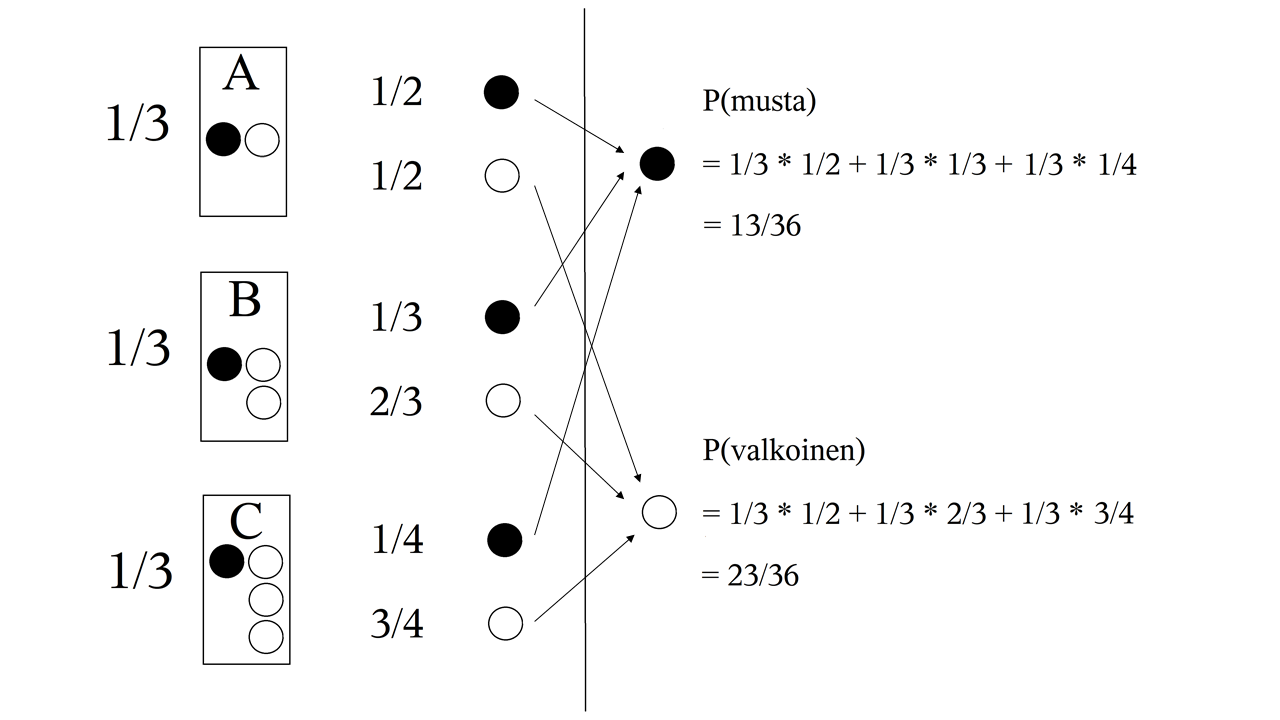
\includegraphics[height = 8cm]{bayes1.png}
\captionof{figure}{The Law of Total Probability.}
\label{kuva:bayes}
\end{center}

Let us then shift the point of view in the example \ref{esim:totalprob}:

\begin{esim}
Continued from the example \ref{esim:totalprob}. Let us assume, that the experiment is conducted behind a curtain: we can not see the box from which the ball is picked -- only the colour of the ball. The ball turns out to be white, that is, we observe that the event $A$ occurs. What is now the probability of event $B_1:$ ''The box picked was number $1$'' given $A$ -- in other words, what is the probability that the picked box was $1$ when we know that the picked ball is was white?

This problem can be solved with the help of the definition of conditional probability  the chain rule of probability:
\[
P(B_1 | A) = \frac{P(B_1\cap A)}{P(A)} = \frac{P(B_1)P(A|B_1)}{P(A)} = \frac{\frac{1}{3} \cdot \frac{1}{2}}{\frac{23}{36}} = \frac{6}{23}. 
\]
Similarly, we are able to calculate the probabilities for the boxes $2$ and $3$:
\[
\begin{split}
P(B_2 | A) &= \frac{\frac{1}{3} \cdot \frac{2}{3}}{\frac{23}{36}} = \frac{8}{23} \\
P(B_3 | A) &= \frac{\frac{1}{3} \cdot \frac{3}{4}}{\frac{23}{36}} = \frac{9}{23}. \\
\end{split}
\]
\end{esim}

The purpose of this example was to showcase an elementary example using a central theorem of probability, the \emph{Bayes' theorem}. The theorem can be utilized in situations where we have observed an event $A$ and when we know the conditional probabilities of $A$ given some partition of the sample space:
\[
P(A|B_i) \quad \text{kaikille} \quad \ i \in \{1, \dots , n\}.
\]
In such case, with Bayes' theorem we are able to calculate the conditional probabilities of events $B_1, \dots , B_n$, given $A$:
\[
P(B_i|A) \quad \text{kaikille} \quad \ i \in \{1, \dots , n\}.
\]

The Bayes' theorem is named after a British mathematician Thomas Bayes, and the theorem can be derived directly from the law of total probability \ref{lause:totalprob}. The theorem is groundbreaking in calculating conditional probabilities, and even a major branch of statistics called the \emph{Bayesian Statistics} or \emph{Bayesian Inference}, is based on this theorem. 

\begin{lause}
Bayes' Theorem.\index{Bayes' Theorem} Let $A$ be an event, for which $P(A) \geq 0$, and $B_1, \dots , B_n$ be a partition of the sample space. Then, a conditional probability for every $B_i$ given $A$ can be calculated using the Bayes' theorem:
\[
P(B_i | A) = \frac{P(B_i)P(A|B_i)}{P(A)} = \frac{P(B_i)P(A|B_i)}{\sum_{j=1}^n P(A|B_j)P(B_j)}.
\]
\end{lause}

\begin{proof}
Again, utilizing the definition of conditional probability and the chain rule, we get
\[
P(B_i | A) = \frac{P(A \cap B_i)}{P(A)} = \frac{P(B_i)P(A|B_i)}{P(A)},
\]
where the latter form can be derived by applying the law of total probability to the denominator.
\end{proof}

Let us next examine a classical example of the Bayes' rule.

\begin{esim}
Let us assume, that a rare disease is carried by $0.1\%$ of the population, and that we have test which can fairly accurately find this test. The sensitivity of this test -- a probability for a positive result for a person carrying the disease -- is $0.95$. The specificity of the test -- a probability for a positive result for a healthy person, is $0.01$. What is the probability that a randomly picked person carries the disease, given that the test result was positive? 

Let us notate $S:$ ''the person is carrying the disease'', $T:$ ''the test result for the person is positive''. From the descriptive text of this example, we find that:
\[
\begin{split}
P(S) &= 0.001 \\
P(S^C) &= 0.999 \\
P(T|S) &= 0.95 \\
P(T|S^C) &= 0.01.
\end{split}
\]
The sample space is partitioned by events $S$ and $S^C$, and thus the probability for a person to be sick, given that the test result was positive, can be calculated using the Bayes' theorem:
\[
\begin{split}
P(S|T) &= \frac{P(S)P(T|S)}{P(S)P(T|S) + P(S^C)P(T|S^C)} \\
	   &= \frac{0.001 \cdot 0.95}{0.001 \cdot 0.95 + 0.999 \cdot 0.01} \approx 0.087.
\end{split}
\]

Let us rephrase the situation in a few words. The probability in question was calculated by researching the ratio of positive result for a sick person and the amount of all positive test results, which consist of the sum of the positives for a sick person and the false positive test results.

The small amount of sick persons within the positive test result can be explained with the small amount of sick persons within the population: despite the sensitivity of the accuracy of the test, it is far more likely that a randomly picked person is healthy \textbf{and} gets a positive test result than a randomly picked person carrying the disease \textbf{and} getting a positive test result.
\end{esim}

\section{Independent Events}\label{independence}

If we were to think about the concept of \emph{independent} events, the intuitive answer would not be too far from the truth. We can, for example, try to remember the examples about the weather or the result of an election: we say that two events are independent, if the first one occurring does not affect to the probability of the second one. There are countless examples which resemble such situation. Lottery numbers in subsequent weeks, a yearly average temperature and the winner of the Finnish ice hockey league, the number of children born in Finland and the average life span of Japan, and so on. The \emph{assumption} of independence is used widely in the applications of probability, for example in statistics and economics -- this assumption makes or breaks multiple central theorems of probability, which is why one should pay attention to it. In addition, it is crucial to note that some events might seem independent, even though they are not. Furthermore, it may be useful to think of an example of two independent events and try to justify why the assumption would hold. Anyways, let us get to the definition:

\begin{maar}\label{maar:indept} \emph{(Two) Independent Events}\index{Independence} The events $A$ and $B$ 
are called independent\footnote{Some literature, or more prominently some lecturers, shorten the word ''independent'' or ''independence'' as indept, or similarly.}, if
\[
P(A \cap B) = P(A)P(B).
\]
In such case we notate $A \independent B$.
\end{maar}

The independence can be equivalently defined with the help of conditional probability, as we are to see in the next theorem. The events $A$ and $B$ are independent, if the probability of $A$ does not change when ''conditionaled'' with event $B$. In other words, the information about $B$ does not change our view on the probability of $A$.

\begin{lause}
\label{lause:conditional_prob}
Let $A$ and $B$ be events such that $P(B) \geq 0$. Now $A \independent B$ if and only if $P(A|B) = P(A)$.
\end{lause}

\begin{proof}
Since the theorem implies equivalency of two statements, we need to show that $A \independent B$ implies if $P(A|B) = P(A)$, and vice versa.

''$\Rightarrow$'': Together with the definition of conditional probability and the events $A$ and $B$ being independent we get that
\[
P(A|B) = \frac{P(A \cap B)}{P(B)} = \frac{P(A)P(B)}{P(B)} = P(A).
\]

''$\Leftarrow$'': From the chain rule and the assumption in the theorem:
\[
P(A \cap B) = P(A|B)P(B) = P(A)P(B).
\]
\end{proof}

\begin{remark}
At this point, the author kindly nudges the reader to check the difference between two \emph{independent} and \emph{disjoint} events. The two concepts are widely mixed up, and proceeding with caution is advised. The chart in the section \ref{axioms} on the interpretation of set theory concepts within the context of probability.
\end{remark}

Let us next illustrate the concept of independent events with few examples.

\begin{esim}\label{esim:independent_events}
Here we introduce an example with independent events and another with dependent events, and also show a straightforward way to find out whether two events are independent or not.

\begin{enumerate}[(i)]
\item Let us toss dice twice, where the sample set is a familiar face of $\Omega = \{1,2, \dots , 6\}^2$. The probabilities for events $A:$ ''The result of the first die is 6'' and $B:$ ''the result of the second die is 6'' are $P(A) = \frac{1}{6}$ and $P(B) = \frac{1}{6}$. Although, it is easy to see that only outcome that satisfies both of these events is $(6,6)$, and thus
\[
P(A \cap B) = \frac{1}{36} = \frac{1}{6} \cdot \frac{1}{6} = P(A)P(B).
\]
From this we see that the events $A$ and $B$ are independent -- that is, the result of the first die does not affect the result of the second die.

\item Let us pick two cards from a standard 52 card deck without replacement. We can choose the set of different 2-permutations as the sample space -- that is, ordered pairs of two cards. We can see that, according to the symmetry of the sample space, the probabilities for events $A:$ ''The first card picked is an ace'' and $B:$ ''The second card picked is ace'' are
\[
P(A) = \frac{4 \cdot 51}{52 \cdot 51} = \frac{1}{13} = \frac{51 \cdot 4}{52 \cdot 51} = P(B).
\]
The number of possible combinations, where both the first and and second cards are aces, is $4 \cdot 3 = 12$, and thus the probability for the intersection of $A$ and $B$ is 
\[
P(A \cap B) = \frac{4 \cdot 3}{52 \cdot 51} = \frac{1}{221} \neq \frac{1}{169}= P(A)P(B),
\] 
from which we infer that the events $A$ $B$ are not independent.

We can also calculate a conditional probability of the second card being ace given that the first card was ace as
\[
P(B|A) = \frac{P(A \cap B)}{P(A)} = \frac{\frac{1}{221}}{\frac{1}{13}} = \frac{1}{17} \neq \frac{1}{13} = P(B).
\]
Do note, that above we used both the definition of independence and the theorem regarding conditional probabilities and independent events, and the result we gained is that the information of the first ace affects the probability of the event $B$.
\end{enumerate}
\end{esim}

\bigskip

Let us next introduce some properties for independence -- these provide to be useful in the future, and most of them are fairly intuitive extensions to the original definition.

\begin{lause}\label{lause:indept_complement}
Independence of a complement. \index{Independence!Complement's} Jos tapahtumat $A$ ja $B$ ovat riippumattomia, myös tapahtumat $A$ ja $B^C$ ovat riippumattomia.
\end{lause}

\begin{proof}
Let us assume that $A \independent B$. Since $A = (A \cap B) \cup (A \cap B^C)$ and that sets $A \cap B^C$ and $A \cap B$ are clearly disjoint, we have
\[
\begin{split}
&P(A) = P(A \cap B) + P(A \cap B^C) = P(A)P(B) + P(A \cap B^C) \quad  \\
\Leftrightarrow &P(A \cap B^C) = P(A) - P(A)P(B) = P(A)[1-P(B)] = P(A)P(B^C),
\end{split}
\]
that is, $A \independent B^C$.
\end{proof}

\bigskip

The definition of independence can be generalized for more than two events. In this case, we require that probabilities of all possible intersections between all events equal the respective product of their probabilities.

\begin{maar}
\emph{Multiple Independent Events} \index{Independence!Multiple Events} The events $A_1, \dots , A_n$ are independent, if  
\[
P\Big( \bigcap_{i \in I} A_i \Big) = \prod_{i \in I} P(A_i).
\]
for all index sets $I \subseteq \{1, \dots , n\}$. Then we notate $A_1, \dots , A_n \independent$.
\end{maar}

For example, the three events $A$, $B$ and $C$ are independent only if the events are pairwise independet with each other -- that is,
\[
\begin{split}
P(A \cap B) &= P(A)P(B) \\
P(A \cap C) &= P(A)P(C) \\
P(B \cap C) &= P(B)P(C),
\end{split}
\]
\textbf{and} in addition 
\[
P(A \cap B \cap C) = P(A)P(B)P(C).
\]

\begin{remark}
Independence for multiple events require, that \emph{all} of the abovementioned independencies are satisfied. With this we want to clarify, that if the events $A$, $B$ and $C$ are pairwise independent (with each other), it does not necessarily follow that $P(A \cap B \cap C) = P(A)P(B)P(C)$.
\end{remark}

\begin{esim}
Let us toss two dice, and notate
\[
\begin{split}
&A \text{: ''the sum of the two dice is 7''}, \\
&B \text{: ''the result of the first toss is 3''}, \\
&C \text{: ''the result of the second toss is 4''}.
\end{split}
\]

Clearly, according to the example \ref{esim:independent_events}, the events $B$ and $C$ are independent. Let us now examine the event $A$. If the result of the first toss is  $k \in \{1, \ldots, 6\}$, then the other toss must result $7-k$ for the sum of the tosses to be $7.$ We quickly notice that $7-k \in \{1, \ldots, 6\}$, and thus despite the result of the first toss, we are able to get a result for the second toss which makes the sum $7.$ This probability is $\frac{1}{6}$, and it can be checked for example with the chart in the example \ref{eq:discrete_prob2}. Thus $P(A)=\frac{1}{6}$. Now
\[
P(A \cap B) = \frac{1}{36} = \frac{1}{6} \cdot \frac{1}{6} = P(A)P(B),
\]
that is, the events $A$ and $B$ are independent. We can equally show that the events $A$ and $C$ are independent. However, we now notice that the event $A \cap B$ could be rephrased as ''the result of the first and second toss is 3 and 4'': now $A \cap B$ = $B \cap C$, after which we see that
\[
P(A \cap B \cap C) = P((A \cap B) \cap C) = P((B \cap C) \cap C) = P(B \cap C) = \frac{1}{6} \cdot \frac{1}{6} = \frac{1}{36}, 
\]
but on the other hand,
\[
P(A)P(B)P(C) = \frac{1}{6} \cdot \frac{1}{6} \cdot \frac{1}{6} = \frac{1}{216},
\]
that is,
\[
P(A \cap B \cap C) \neq P(A)P(B)P(C)
\]
which means that the events $A$, $B$ and $C$ are not independent. 
\end{esim}

\section{Bernoulli Trials}\label{toistokokeet}

\emph{In this section we discuss an often-occurring random experiment: repeated yes-or-no trial, where the trials are independent.}

Sometimes it is useful to think about a situation, where we want to repeat the random experiment $n$ times. To make this section meaningful to the scope of this course, let us only examine situations where the experiments are independent. And to make matters more simple (and to limit ourselves to an useful special case), we are only interested in whether a single event $A$ happens or not, or that whether a single trial is successful or not -- this is, each experiment can be modelled to have a boolean-valued outcome, $0$ or $1$. If we denote $P(A)=p$, $P(A^C) = 1-p :=q $, and furthermore if we denote

\begin{align*}
B_k = "A \text{ occurs exactly} k \text{ times}",
\end{align*}
we have enough tools to calculate $P(B_k)$.
 	
As we have done before, before defining the concept of Bernoulli Trials, let us examine an example:

\begin{esim}\label{toistoesim}
Let's examine a situation where we want to repeat a tossing of a single die $5$ times, and let us further assume that we would be interested about the amount that number $6$ occurs. Now $A=$ ''single toss results in 6'', and $B_3=$ ''out of five tosses $3$ result in sixes''. In addition,  $p=1/6$ and $q=5/6$. Then, to model a Bernoulli trial with $5$ repeats, we choose all sequences $(\omega_1,\omega_2,\dots,\omega_5)$, where $\omega_i \in \{A,A^c\}$ for all $i\in \{1,2,3,4,5\}$, to be the outcomes in the sample space.

Since the single tosses are independent, a probability for each sequence resulting in $3$ times of sixes and $2$ times of non-sixes, is
\begin{align*}
p^3 q^{2} = \Big(\frac{1}{6}\Big)^3 \Big(\frac{5}{6}\Big)^2.
\end{align*}

In addition, we have a total of $\binom{5}{3}$ sequences, where the result is $3$ sixes. Furthermore, due to the rule of product, we get
\begin{align*}
P(B_3)= \binom{5}{3}\Big(\frac{1}{6}\Big)^3 \Big(\frac{5}{6}\Big)^2 \approx 0.032.
\end{align*}
\end{esim}

To generalize this example, let us ascend from the realm of coin tosses and $k=3$, and state how the general probability $P(B_k)$ behaves:

\begin{lause}\label{lause:toistokoe}
Bernoulli Trial\footnote{Sometimes referred to as the binomial trial.}. \index{Bernoulli Trial}\index{Binomial Trial} Let us denote $P(A)=p$. Then, in a  $n$ times repeated \emph{Bernoulli Trial}, the probability for event $B_k= "A \text{ occurs exactly } k \text{ times}"$ is 
\begin{align*}
P(B_k)= \binom{n}{k}p^k q^{n-k},
\end{align*}
where $k=0,1,\dots,n$ ja $q=1-p$.
\end{lause}

\begin{proof}
The proof is as we derived the example \ref{toistoesim}.
\end{proof}

Let us now sit down for a moment and memorize the concept of sampling \ref{sampling}. It is easy to see that in sampling with replacement we execute subsequent, independent random exams, and thus it would be fair to think that we can utilize the Bernoulli trial to calculate probabilities in such cases.

\begin{esim}
Continued from the part $(ii)$ of example \ref{esim:balls}. We can interpret sampling with replacement as a $n$ times repeated Bernoulli trial, where $A:$ ''randonly picked ball is white'', and furthermore $p = K/N$, the number of white balls divided by the number of all balls in a box, with the notations introduced in the theorem \ref{lause:sampling}.

There are $5$ white balls and $3$ black balls in a box. Let us pick $4$ balls out of the box with replacement. What is the probability to pick no more and no less than $2$ white balls?

Let us denote $B_k$ as ''a total of $k$ white balls was picked.'' Now $p = \frac{5}{8}$, and according to the \ref{lause:toistokoe} we have
\[
P(B_2) = \binom{4}{2} \Big( \frac{5}{8} \Big) ^2 \Big( \frac{3}{8} \Big) ^{4-2} \approx 0.3296,
\]
which is exactly the same answer as the one we derived back in the example \ref{esim:balls}.
\end{esim}

\bigskip

A Bernoulli trial, or a binomial trial, can be further modelled with so-called  \emph{Binomial Distribution}, which is further examined in section \ref{binomial_distr}. A basis for examining distributions, \emph{random variables}, is discussed in-depth in the next chapter. As we will see, the notions of this chapter, conditional probability and independence, in addition to the Bernoulli trial, can be generalized to cover random variables. 

\section{Exercises}
\begin{enumerate}
\item Let us toss two dice. What is the probability that at least one of the dices is $6$, given that both tosses had a different result?
\item Let us assume that $A \subset B$. Express the following event as clearly as possible:
\begin{enumerate}[a)]
    \item $P(A|B)$
    \item $P(A|B^C)$
    \item $P(B|A)$
    \item $P(B|A^C)$
\end{enumerate}
\item There are $6$ red and $9$ white balls in a box. In a random experiment, we are to pick $3$ balls without replacement. Calculate the following probabilities:
\begin{enumerate}[a)]
    \item all picked balls are red, given that at at least one picked ball is red,
    \item all picked balls are red, given that all balls share the same colour, 
    \item 1 of the picked balls is red and 2 are white, given that not every ball shares the same colour.
\end{enumerate}
\item Let us toss two dice. Let $A:$ ''the sum of the two tosses is 6'' and $B:$ ''the result of the first toss is $4$''. Does $A \independent B$ hold? Answer without using the definition of independence.
\item A fair coin is tossed twice. Let us define events $A$, $B$ and $C$ in a following way:
\begin{itemize}
\item A: The first toss is heads,
\item B: The second toss is heads, a
\item C: Both tosses land on the same side.
\end{itemize}
Show that the events $A$, $B$, and $C$ are pairwise independent, but not independent -- that is, show that  $A\independent B$, $A \independent C$ and $B \independent C$, but $A$, $B$ and $C$ are not independent.
\item Mrs. K works at Mint of Finland. At the end of their shift, all employees are randomly inspected. The probability of an inspection for each employee is $0.03$. What is the probability for Mrs. K being inspected 
\begin{enumerate}[a)]
\item exactly once,
\item at least once, or
\item more than once
\end{enumerate}
during her 5-day working week? 
\item In the box $A$ there are 2 white and 3 black balls, in the box $B$ there are one white and 4 black balls, and in the box $C$ there are 5 white and 2 black balls. Let us pick one ball, but before picking we choose box $A$ with probability $\frac{3}{6}$, box $B$ with probability $\frac{2}{6}$ and box $C$ with probability $\frac{1}{6}$. Assuming that the pick is random, what is the probability that the picked ball is white?
\item A tale is told that in his old days, Robin Hood had lost his sight. To spend his casual days of retirement, Hood shoots with a box (towards a target) and his grandchild lets him know, whether he hit or missed. Probability for Hood to hit is $0.3$, and a probability that the grandchild announces the shot correctly is $0.8$. What is the probability that Hood hit his target, given that the grandchild announced it so?
\end{enumerate}

%%%%%%%%%%%%%%%%%%%%%%%%%%%%%%%%%%%%%%%%%%%%%%%%%%%%%%%%%%%%%%%%%%%%%%%%%%%%%%%

\chapter{Random Variables}\label{sm}

Previously on this course, we have examined various random experiments and their possible outcomes -- however, in many cases we are interested in the theoretical properties of these random experiments, even before these experiments are conducted. In other cases, we might be interested in a transformation (function) of an outcome. For example, we might be interested in the sum of two dice, rather than the outcomes of single dice which form the particular sum\footnote{In other words, for us the interesting information could be that the sum is $6$, not the particular parts of the sum: 2 and 4, 1 and 5, 5 and 1, and so on.}. Alternatively, when flipping a coin, we might be more interested in the ratio of heads in hundred flips, than the particular sequence of heads and tails which happen to be the result. In these situations, the concept of \emph{random variables} becomes handy and essential.

To carry on, in many of our examples we have examined a result of a single die toss: this single result, or the number representing the result, is in fact a random variable, even though we have not represented it as such. As always, defining random variables is crucial in order to further develop the concept to cover for example \emph{distributions}, their \emph{statistics}, such as \emph{expected value} and \emph{deviation}, in addition to expand the number of cases we are able to examine mathematically.

We call a function random variable, if the function maps a real valued number to every possible outcome of an random experiment. To further explain, a random variable is a function and its value will be assigned by the outcome of the random variable. In this section we are going to examine a special case of random variables, \emph{discrete random variables.} As is right and justified, let us begin by defining these concepts and carry on with some elementary examples.

\begin{maar} \label{maar:rv}
\emph{A Random Variable}\footnote{Often abbreviated as r.v.} \index{Random Variable} Let $(\Omega, \F, P)$ be a probability space. A function\footnote{Do note, however, that this definition is not mathematically exhaustive, so to say. For the scope of this material, this definition is adequate, but let us let you know that for an exhaustive definition we require that the function $X$ is \emph{Borel-measurable}. By this we mean that is for every measurable Borel Set -- roughly speaking, for every countable union and intersection of some ''smooth'' sets -- we require that the preimages of these sets are an events in the sample space, that is, $X^{-1}(B) \in \F$ for all ''smooth'' $B\subseteq \R$.} $X:\Omega \rightarrow \R$ is\footnote{Usually we use capital letters, such as $X$ and $Y$, to notate random variables. This information becomes crucial when moving to statistical inference, where the values of the random variables observed as data are denoted with non-capital letters: the random variable $X$ has some probability distribution, which then is observed as a data $x$.}\label{footer:capitalx} called a  \emph{random variable}. 
\end{maar}

Often, we use a shorthand notation $X(\omega)=X$.

\begin{remark}
At this point it should be clarified that under the previous definition, a random variable is not technically \emph{random} or a \emph{variable}\footnote{This is one of the author's favourite gimmicks in probability -- it sounds like a joke, and to some audiences it can be described as hilarious. However, despite the goofiness in the front, the etymology can be justified.}. Rather, it is a deterministic function in a sense that it always maps a predetermined real valued number to each outcome in a sample space. It might be justified to use a moment to wonder: why do we consider such function a useful tool for discussing random events?
\end{remark}

Let us now define a special case of random variables, where we limit the set of values of this function.

\begin{maar}
\emph{A Discrete Random Variable.}\index{Random Variable!Discrete} \index{Discrete Random Variable} A random variable $X: \Omega \rightarrow \R$ in the probability space $(\Omega, \F, P)$ is called a \emph{discrete random variable}, if the set of its possible values $X(\Omega)$ is countable -- that is, finite or countably infinite.
\end{maar}

In layman's terms this means that all possible values of this random variable can be listed, at least in theory. Examples of discrete random variables can be a result of a die toss with possible values being $\{1, \ldots, 6\}$, or earth's population count in a given moment with possible values of all natural numbers $0,1,2,\ldots$.

\begin{esim}
\label{discrete_rv1}
Let us now examine three elementary examples on discrete random variables.. 
\begin{enumerate}[(i)]
\item Tossing a single die. For a sample space $\Omega = \{1,2,3,4,5,6\}$, let us define a random variable $X:\Omega \rightarrow \R, \,\, X(\omega) = \omega$. Now, random variable $X$ represents a result of a tie doss. For example, the set $\lbrace X(\omega)=X=3 \rbrace$ represents an event, where the result of a die toss turns out to be $3$.

The value set of this random variable is $X(\Omega) = \{1,2,3,4,5,6\}$, which is finite, and thus we are looking at a discrete random variable.

\item Tossing two dice. For a sample space $\Omega = \{(a,b) : a,b \in \{1,2,3,4,5,6\}\}$, let us define a random variable $Y(\omega) = Y(a,b) = a + b$. Now the random variable $Y$ represents the sum of the results of these two tosses.

Now, the value set of $Y$ is $Y(\Omega) = \{2,3, \dots , 12\}$, and thus the random variable $Y$ is also a discrete random variable.

\item\label{esim:passthepig2} Pass the pigs (see earlier example \ref{esim:passthepig1}). Let the sample space be $\Omega = \{\omega_1, \dots , \omega_5\}$ and assign the probabilites as following: 
\bigskip

\begin{tabular}{l l L{4cm} l l}
\toprule
& Name & Position & Points & $P(\omega_i)$\\
\midrule
$\omega_1$ & Side & Lying on its side  & 0 p. & 0.651\\
$\omega_2$ & Razorback & Lying on its back & 5 p. & 0.225\\
$\omega_3$ & Trotter & Standing upright & 5 p. & 0.088\\
$\omega_4$ & Snouter & Leaning on its snout & 10 p. & 0.030\\
$\omega_5$ & Leaning Jowler & Resting on its snout and ear & 15 p. &  0.006\\
\bottomrule 
\end{tabular}

\bigskip

Let us define random variable $Z:\Omega \rightarrow \R$ as the points awarded by each landing position -- outcome of a sample space -- of the pig: for example $Z(\omega_1) = 0$. Now the value set of $Z$ is $Z(\Omega) = \{0,5,10,15\}$, which makes $Z$ a discrete random variable.  
\end{enumerate}
\end{esim}

\bigskip

An event where $X$ gets values from the set $B \in \R$ is notated in a following way:
\[
\{X \in B\} = \{\omega \in \Omega : X(\omega) \in B\}. 
\]
Now, the probability that this event occurs can be notated in following ways:
\[
P(X \in B) = P\{X \in B\} = P(\{X \in B\}) = P(\{\omega \in \Omega : X(\omega) \in B\} ). 
\]
Again\footnote{See remark \ref{huom:brackets}} we tend to drop out the second set of brackets to loosen up the notation style. In this material, hereafter we notate $P(X \in B)$.

Let us next introduce the concepts of \emph{probability distribution} and \emph{probability mass function} by first defining them, and afterwards somewhat surprisingly illustrating them in practice via examples.

The probabilities of possible values of the random variables are modelled with the help of distributions. The probability distribution and the probability mass function defining the distribution tell us the probabilities of each outcome for a single random variable. Likewise when defining probability as a set mapping defined for the subsets of the sample space -- events --, we define the distribution of a random variable as a set mapping, which is defined for the subsets of the random variable's value set.

\begin{maar}
\emph{Probability Distribution of a Random Variable.}\index{Distribution} \index{Random Variable!Distribution} Let $X: \Omega \rightarrow \R$ be a random variable. Now the distribution of $X$ is a set mapping 
\[
P_X := P(X \in B),
\]
which is defined for every ''smooth''\footnote{Again, more specifically for the real-valued Borel-sets.} subset $B \subseteq X(\Omega)$ of the value set of $X$.
\end{maar}

\begin{remark}
It can be shown that for a random variable $X$, its distribution $P_X$ satisfies the probability axioms (PROB1)--(PROB3), and thus spans a probability function in the value set of the random variable. This leads to a surprisingly useful remark that we don't have to separately define the probability space and the sample set in many applications, and instead we define only the random variable and its distribution. It can be thought that the sample space is the value set of the random variable $X(\Omega)$, the events are its subsets and that the probability function is given by the distribution $P_X$.
\end{remark}

Now that we have established a distribution for random variables. Let us now move to the concept of a probability mass function, which defines more useful way for defining probabilities for each event.

\begin{maar}
\emph{Probability Mass Function.}\footnote{Often abbreviated as pmf. Do note that with probability mass function we refer to the mass function of a discrete random variable, and more generally we use the word probability density function to refer to the distributions of continuous random variables.} \index{Probability Mass Function} \index{Distribution!Probability Mass Function} A function $f:\R \rightarrow \R$ is a probability mass function for a random variable $X: \Omega \rightarrow \R$, if
\[
f(x) = P(X =x)  \quad \text{for all} \quad x \in \R.
\]
Technically the probability mass function is defined for all real valued numbers, but the value of the function is zero outside the value set of $X$\footnote{In a practical sense, this means that an event, where the random value attains a value outside its value set, is impossible. For example, we can not throw a regular 6-sided die with a number 7 as a result.}:
\[
f(x) = 0 \quad \text{for all} \quad x \notin X(\Omega).
\]
When handling several random variables simultaneously, we refer to a specific probability mass function with a subindex to avoid confusion:
\[
f_X(x) = P(X=x).
\]
\end{maar} 

Again, time for a small remark.

\begin{remark}
We have now learned that a probability mass function tells a probability for an event that the value of a random variable $X$ is $x$\footnote{To continue from a previous footnote regarding capital letters, now that we have defined the concepts of a distribution and a random variable: intuitively we can justify the notations in a following way. Let us make a random experiment, and assume that the outcome of this experiment is modelled as a random variable $X$. Now, before the experiment is conducted, the value of $X$ is still unknown, and thus random to observers. We then notate $x$ as the result of the random experiment, which is observed and given to us by the gracious Miss Fortune. Then the probability mass function $f(x)$ tells the probability for an yet-observed number $X$ to be observed as $x$ after the random experiment -- $P(X=x)$.}.
\[
f(x) = P(X =x)  = P(\{\omega \in \Omega : X(\omega) = x\}).
\]
When $(\Omega, \F, P)$ is the original probability space, then $\{X=x\} \in \F$, and the $P$ above is the probability of this original probability space. Thus, the probability mass function gives us the probabilities for the values of the random variable as the original probabilities of the events in the sample space. 
\end{remark}

In the case of a discrete random variable, as we saw with discrete probability\footnote{See theorem \ref{lause:discrete_prob}.}, the situation simplifies: now the probabilities of an each element in a value set span the probability distribution in a unique way, and the probabilities for each event are given as the sums of the probabilities of single values:
    
\begin{lause}
Let $X$ be a discrete random variable and $f$ its probability mass function. Now $f$ defines the distribution of $X$ with
\[
P(X \in B) = \sum_{x \in B} f(x).
\]
\end{lause}

\begin{proof} Left as an exercise. This can be solved by using the law of total probability for the sample space $\Omega = \{x_1, x_2, \dots\}$, using the set 
\[
\{X \notin X(\Omega)\}, \{X = x_1\}, \{X = x_2\}, \dots
\]
as the partition.
\end{proof}

Let us illustrate the previously defined concepts with a few examples.

\begin{esim}
\label{discrete_rv2}
Continued from the example \ref{discrete_rv1}. Let us define the probability mass functions for the previously defined random variables.
\begin{enumerate}[(i)]
\item Tossing a single die. Let us assume a symmetric probability space -- that is, the probabilities for every outcome are 
\[
P(\omega) = \frac{1}{6}.
\]
Now we can shorten the notation as $\{\omega \in \Omega : \omega = x\} := \{X = x\} := \{x\}$, and thus
\[
f_X(x) = P(X=x) = P(x) = \frac{1}{6} \quad \text{for all} \quad x \in X(\Omega).
\]
In addition $f(x) = 0$ for all $x \notin X(\Omega) = \{1,2, \dots , 6\}$; in many occasions this is not separately mentioned.

We can illustrate the distributions defined by the probability mass functions with a graph, where in the x-axis is the value set of $X$ and in the y-axis the respective probabilities $P(X=x_i)$. Now the graph of a probability mass function in the case of single die toss looks like this:

\begin{figure}[!h]
\centering
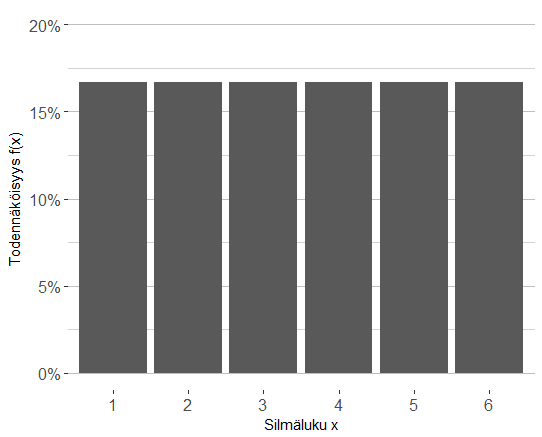
\includegraphics[height = 9cm]{noppa.png}
\caption{A distribution of a single die toss (x-axis is the value set and y-axis is the respective probability).}
\end{figure}

\item Tossing two dice. Let us again assume a symmetric sample space, which means that in this case, the probabilities for each outcome are 
\[
P(\omega) = \frac{1}{36}.
\]
Now the probability mass function is calculated by counting the outcomes which represent each outcome:
\bigskip

\begin{tabular}{l l l}
\toprule
 $y$ & Favourable Outcomes  & $f_Y(y)$ \\
\midrule
 2 & $(1,1)$ & $1/36$ \\
 3 & $(1,2), (2,1)$ & $2/36$ \\
 4 & $(1,3), (2,2), (3,1)$ & $3/36$ \\
 5 & $(1,4), (2,3), (3,2), (4,1)$ & $4/36$ \\
 6 & $(1,5), (2,4), (3,3), (4,2), (5,1)$ & $5/36$ \\
 7 & $(1,6), (2,5), (3,4), (4,3), (5,2), (6,1)$ & $6/36$ \\
 8 & $(2,6), (3,5), (4,4), (5,3), (6,2)$ & $5/36$ \\
 9 & $(3,6), (4,5), (5,4), (6,3)$ & $4/36$ \\
 10 & $(4,6), (5,5), (6,4)$ & $3/36$ \\
 11 & $(5,6), (6,5)$ & $2/36$ \\
 12 & $(6,6)$ & $1/36$ \\
 \bottomrule 
\end{tabular}

\bigskip

The graph for the two dice setting is presented below. From the graph we can easily see, that for example number 7 is the most probable sum in tossing two dice -- in other words, it is the \emph{mode} of this distribution.

\begin{center}
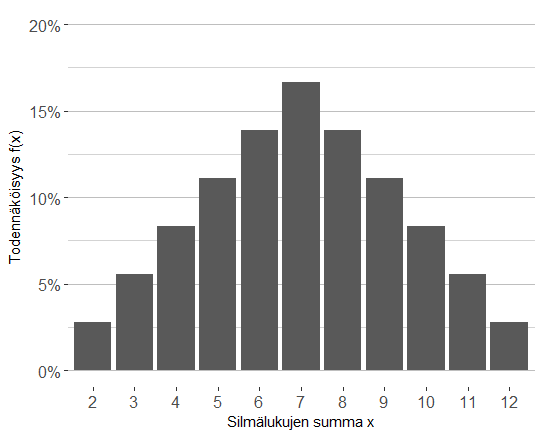
\includegraphics[height = 9cm]{noppa2.png}
\captionof{figure}{Distribution of the sum of the results in a two dice toss (x-axis represents the sum and y-axis represents the value of the probability mass function).}
\end{center}

\bigskip

\item Pass the pig. Again, the probability mass function of our random variable is derived by summing the probabilities of each outcome satisfying each value of the random variable:
\bigskip

\begin{tabular}{l L{4cm} l l}
\toprule
 $z$ & Favourable Outcomes & Name & $f_Z(z)$ \\
\midrule
0 & $\omega_1$ & Side & $0.651$ \\
5 & $\omega_2, \omega_3$ & Razorback, Trotter & $0.313$ \\
10 & $\omega_4$ & Snouter & $0.030$ \\ 
15 & $\omega_5$ & Leaning Jowler & $0.006$ \\ 
\bottomrule 
\end{tabular}

\begin{center}
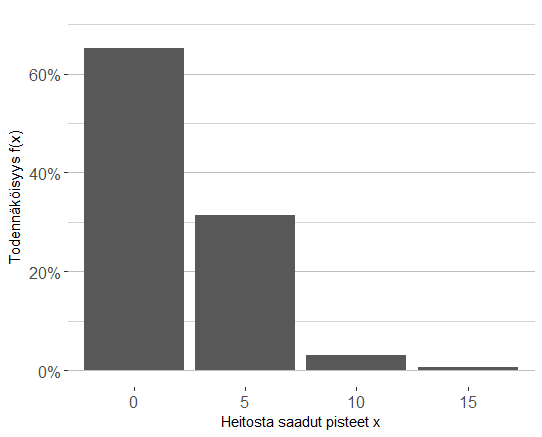
\includegraphics[height = 9cm]{sika.png}
\captionof{figure}{Distribution of points in a single pig pass (x-axis represent the points and y-axis represent the probability mass function).}
\end{center}

\bigskip

\end{enumerate}

\end{esim}

If the reader paid attention, they would notice that in each of the previous cases, the probabilities given by the probability mass function for each random variable sum up to $1.$ This is a general property, and a very useful one, which can be generalized as in the following theorem:

\begin{lause}
\label{lause:pmf_properties}
Properties of a Probability Mass Function. Let $X:\Omega \rightarrow \R$ be a discrete random variable. Now, for its probability mass function $f$ holds that:
\begin{enumerate}[(i)]
\item $f(x) \geq 0$ for all $x \in \R$.
\item jos $f(x)>0$, $x \in X(\Omega) = \{x_1, x_2 \dots\}$ -- that is, $x$ belongs to the value set of $X$.
\item $\sum_{i=1}^\infty f(x_i) = 1$.
\end{enumerate}
\end{lause}

It can be shown, that these properties also hold ''the other way around'': every non-negative function $f:\R \rightarrow \R$, which attains positive values in finite or countable finite set and sums up to one over all its values, is a probability mass function for some \emph{unique} random variable.

From the probability mass function, we are able to derive a \emph{cumulative distribution function}, which tells us the cumulative probability up until some point. Whereas the probability mass function tells the probability for the event to occur as an exactly some given value, the cumulative distribution function tells us the probability that the result of the event is \emph{at most} some certain value. Let us next present the definitions for the cumulative distribution function, as a general case and with discrete random variables.

\begin{maar} \label{maar:cdf}
\emph{Cumulative Distribution Function.}\footnote{Shortened often as CDF.} \index{Cumulative Distribution Function} \index{Distribution!Cumulative Distribution Function} Function $F:\R \rightarrow \R$ is a cumulative distribution function for a random variable $X$, if
\[
F(x) = P(X \leq x) \quad \text{for all} \quad x \in \R.
\]
\end{maar} 

\begin{maar}
\emph{Discrete Cumulative Distribution Function.}\index{Cumulative Distribution Function!Discrete} Function $F:\R \rightarrow \R$ is a cumulative distribution function for a \emph{discrete} random variable $X$, if
\begin{align*}
F(x)=P(X\leq x) = \sum_{x_k \leq x} P(X = x_k) = \sum_{x_k \leq x} f(x_k),
\end{align*}
where $k\in\{0,1,2,\dots,x\}$. That is, the cumulative distribution function for a discrete random variable is attained as the sum of the respective probability mass functions $f$. Since the value set for the discrete random variable is at most countable, the sum in question exists and is countable.
\end{maar}

Let us next examine an example.

\begin{esim} \label{esim:discrete_rv_cdf}
Tossing a single die, continued from the part $(i)$ of the examples \ref{discrete_rv1} and \ref{discrete_rv2}. From the graph of $X$'s (a random variable for a result of a single toss) cumulative distribution function we see, that for example the probability of the toss resulting in 3 or less is $0.5$ and the probability of the toss resulting 6 or less is $1$ -- that is, it is \emph{certain} that the reuslt is 6 or less.

\begin{center}
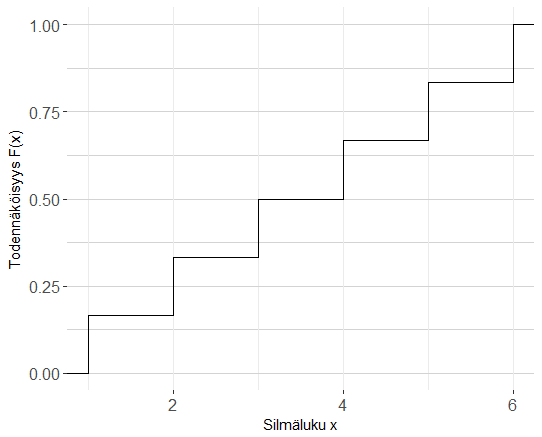
\includegraphics[height = 9cm]{noppa_cdf.png}
\captionof{figure}{CDF for a single die toss (x-axis represents the result in numbers and y-axis the value of CDF).}\label{kuva:nopanheiton_kf}
\end{center}

\end{esim}

The following properties introduced in a following theorem can be derived directly from the definition of a cumulative distribution function:

\begin{lause}\label{lause:cdf_properties} 
Properties for a Cumulative Distribution Function. The cumulative distribution function $F:\R \rightarrow \R$ of a random variable $X$ has the following properties:
\begin{enumerate}[(i)]
\item $F$ is an increasing function
\item $F$ is right-continuous -- that is,
\[
F(x+) = F(x), \quad \text{for all } x \in \R.
\]
\item $F(-\infty) = 0$ ja $F(\infty) = 1$. 
\end{enumerate}
\end{lause}

\bigskip

And as with the probability mass function, also this definition works vice-versa: if any function $F$ has these properties, then there exists a random variable $X$, such that $F(X)$ is a cumulative distribution function for $X$. For example, the reader can verify from the picture \ref{kuva:nopanheiton_kf} that the CDF in the example \ref{esim:discrete_rv_cdf} satisfies the properties in the theorem  \ref{lause:cdf_properties}.

The cumulative distribution functions are especially useful in the domain of \emph{continuous random variables}, which are discussed in the next chapter. For discrete random variables, the concept is not as useful, since the calculation of the sum involved can be rather difficult when the amount of summed terms increase drastically. Before the age of computers and the surge of computing power, this was also a practical issue. Because of this, it lead to several theories where the sums of probability mass functions were approximated with other distributions. We'll get back to this notion later. Let us now introduce some well-known distributions!

\section{Discrete Distributions}

\emph{This section is a very useful one, where we will introduce various known distributions. In case of an emergency, the section works also quite well as a cheat sheet.}

In the previous section, we learned that every non-negative function $f:\R \rightarrow \R$, which sums to one over all of its indexes and gains positive values only in a countable number of sets, is a probability mass function for a discrete random variable. Roughly speaking, this means that there is an infinite amount of different discrete probability distributions. Some of them are useful, some of them are only mathematical curiosities, and some of them are actually used in solving practical problems. Let us next introduce some of the most important discrete distributions.

\subsection{Discrete Uniform Distribution}

\begin{maar}\label{discrete_uniform_distr}
Random variable $X$ follows a \emph{discrete uniform distribution} \index{Distribution!Discrete Uniform}\index{Uniform Distribution!Discrete} over a support $\{1, \dots, n\}$, if its probability mass function is
\[
f(k) = P(X=k) = \frac{1}{n} \quad \text{for all} \quad k \in \{1, \dots, n\}. 
\]
\end{maar}

In the part $(i)$ of examples \ref{discrete_rv1} and \ref{discrete_rv2}, the random variable $X$ follows a discrete uniform distribution over a set $\{1, \dots, 6\}$. Every possible value of a random variable following a discrete uniform distribution are equally likely.

\subsection{Bernoulli Distribution}\label{bernoulli_distr}

\begin{maar}
Random variable $X$ follows a \emph{Bernoulli distribution}\index{Distribution!Bernoulli} \index{Bernoulli Distribution} with a parameter\footnote{We call some number a parameter when it is used as an argument to fully define a unique probability mass function or some other function within the area of probabilities.} $p \in (0,1)$ if its probability mass function is 
\[
f(k) = P(X=k) = p^k(1-p)^{1-k}, \quad \text{where } k \in \{0, 1\}.
\]
In such case we notate $X \sim \text{Bernoulli}(p)$.
\end{maar}

With a Bernoulli distribution we can model a random experiment, where we have two alternative outcomes, a success ($X=1$) and a failure ($X=0$), and the probability for success is $p$. For example in a coin toss, we can notate heads with $1$ and tails with $0$ -- now the outcome of the result is following a Bernoulli distribution with a parameter $p=\frac{1}{2}$. Likewise, if we toss a die, and define the result $6$ as a success and other results as a failure, the result of a die toss follows a Bernoulli distribution with parameter $\frac{1}{6}$. 

\begin{esim}
Flipping a coin. Lets notate heads with $1$ and tails with $0$. Now, from the pmf of a Bernoulli distribution we see that the probability for heads is 
\[
f(1) = 0.5^1 \cdot 0.5^0 = 0.5.
\]
We see, that in the case where the coin is fair, the parameter $p$ has to be $0.5$. If we had a biased coin, we could for example model a toss with a Bernoulli distribution with parameter $p=0.7$, and now it would hold that $f(1) = 0.7$ and $f(0) = 0.3$. From this we see, that Bernoulli distribution's probability mass function gives us the probabilities for success (= 1) or a failure (= 0). 
\end{esim}

\subsection{Binomial Distribution}\label{binomial_distr}

\begin{maar}
Random variable $X$ follows a \emph{Binomial Distribution}\index{Distribution!Binomial}\index{Binomial distribution} with parameters $n \in \{1,2, \dots \}$ and $p \in [0,1]$, if it has a probability mass function of a form
\[
f(k) = P(X=k) = \binom{n}{k} p^k (1-p)^{n-k} \quad \text{for all} \quad k \in \{0,1, \dots, n\}.
\]
In this case, we notate $X \sim \text{Bin} (n,p)$.
\end{maar}

The generalization of Bernoulli distribution is called binomial distribution: the binomial distribution can be used in situations, where the same random experiment, such as a coin toss, is repeated many times -- that is, binomial distribution can be used to model the number of successes in a Bernoulli trial, which we discussed in the section \ref{toistokokeet}.

\bigskip

Let us examine the part $(ii)$ of the example \ref{esim:balls}. Let the amount of white balls picked in a sample of four balls be the random variable $X$. Now $X$ follows a binomial distribution with parameters $n=4$ and $p = \frac{5}{8}$. This can be seen easily by comparing the probability mass function of the binomial distribution and the probability calculated in the example.

Likewise, we can model the amount of white balls picked in a sample of $n$ balls, as in the part $(ii)$ of the theorem \ref{lause:sampling} with random variable $X$. Now $X$ follows a binomial distribution with parameters $n$ and $p = \frac{K}{N}$, where $K$ is the amount of white balls in a box, and $N$ is the total amount of balls in every box. It is easy to see, that the formula in the theorem truly is the probability mass function of a binomially distributed random variable.

\begin{remark}
We only now stated that the binomial distribution is a generalisation of a Bernoulli distribution. This can be seen by noticing that a random variable following Bernoulli distribution with parameter $p$ happens to also be following Binomial distribution with parameters $(1,p)$.

Since the probability mass functions define the random variables in a unique way, this can be verified by checking that the pmf's are equal with the respective parameters.
\end{remark}

\subsection{Hypergeometric Distribution}

\begin{maar} 
Random variable $X$ follows a \emph{Hypergeometric Distribution} \index{Distribution!Hypergeometric}\index{Hypergeometric Distribution} with parameters $N \in \{1,2, \dots\}$ and $n,K \in \{1, \dots, N\}$, if its probability mass function is of form 
\[
f(k) = P(X=k) = \frac{\binom{K}{k} \binom{N-K}{n-k}}{\binom{N}{n}} \quad \text{for all} \quad k \in \{0,1, \dots , n\}. 
\]
In this case we notate
\[
X \sim \text{Hyperg}(N,K,n).
\]
\end{maar}

With hypergeometric distribution we are able to model sampling without replacement. If the amount of white balls picked in the part $(i)$ of example \ref{esim:balls} is modelled with a random variable $X$, it follows a hypergeometric distribution with parameters $N = 8$, $K=5$, and $n=4$. Likewise in the part $(i)$ of theorem \ref{lause:sampling}, the amount of white balls picked can be modelled with hypergeometric distribution.

Again, a remark will be useful to enhance the learning process.

\begin{remark}
Do note that since by the definition of binomial coefficient, the value of  $\binom{x}{y}$ is zero if $y>x$. From this it follows that the value set of hypergeometric distribution only consists of $k \in \{0,1, \dots , n\}$, for which $k \leq K$ and $n-k \leq N-K$. This is sort-of trivial, and it means that if the balls are not replaced after each pick, we can not pick more white or black balls from the box than what there existed in the first place.
\end{remark}

\subsection{Geometric Distribution}

\begin{maar}
Random variable $X$ follows a \emph{Geometric Distribution}\index{Distribution!Geometric}\index{Geometric Distribution} with parameter $p \in (0,1)$, if its probability mass function is of form
\[
f(k) = P(X=k) = p(1-p)^k \quad \text{for all} \quad k \in \N.
\] 
In this case we notate
\[
X \sim \text{Geom}(p).
\]
\end{maar}

As all the previous distributions, the geometric distribution will prove itself useful. Let us repeat a random experiment with a success probability of $p$, until we obtain our first success. Then, if random variable $X$ describes the amount of failures until the first success occurred, follows a geometric distribution with parameter $p$. The intuition behind the probability mass function can be found when thinking that in such repetition of random experiments, there first is $k$ failures with probability $(1-p)$, and then a success with probability $p$. Now, from the rule of product and the definition of probability mass function, we obtain the probability mass function for geometric distribution.

In theory, we might have infinite failures before the first success -- the value set of a random variable following a geometric distribution is the set of natural numbers $\mathbb{N}$.

\begin{esim}
Let us toss a die, until we obtain the first result of $6$. Let us denote the number of tries before the first six with $X$ (note that the toss where we obtain six is not included). Now $X$ is a random variable following a geometric distribution with parameter $p = \frac{1}{6}$. The probability mass function is now easy to infer: 
\begin{itemize}
\item $X=0$, that is, the first toss results in six: $P(X=0) = \frac{1}{6} = p(1-p)^0$.
\item $X=1$, that is, the first toss results in some other outcome than six, and the second results in six: $P(X=1) = \frac{5}{6} \cdot \frac{1}{6} = p (1-p)^1$
\item $X=2$, if the first two tosses do not result six, and the third one does: $P(X=2) = \left(\frac{5}{6}\right)^2 \cdot \frac{1}{6} = p(1-p)^2$. Snd so on...
\end{itemize}
\end{esim}

\begin{remark}
It can be easily verified, that a random variable following geometric distribution also satisfies the properties in the theorem \ref{lause:pmf_properties}. In particular, we see that by abusing the formula for geometric sum, which diverges, since $1-p < 1$, that the values of the probability mass functions sum up to one:
\[
\sum_{k=0}^\infty p(1-p)^k = p \frac{1}{1- (1-p)} = 1.
\]
\end{remark}

\begin{remark}
Do note, that the notation and the parametrisation of the geometric distribution vary across different sources. In some literature, the probability mass function is notated as 
\[
f(k) = p(1-p)^{k-1},
\]
and in such case the random variable deciphers the order number of the first success, rather than the amount of failures in the trials.
\end{remark}

\subsection{Poisson distribution}

\begin{maar}
Random variable $X$ follows a \emph{Poisson distribution}\index{Distribution!Poisson}\index{Poisson Distribution} with parameter $\lambda > 0$, if its probability mass function is of form
\[
f(k) = P(X=k) = e^{-\lambda} \frac{\lambda^k}{k!} \quad \text{for all} \quad k \in \N.
\]
In such case we notate 
\[
X \sim \text{Poisson}(\lambda).
\]
\end{maar}

With Poisson distribution, we can model the amount of events during a constant time or unit interval, if we assume the events to be independent and their expected occurrence rate to be constant within these intervals. For example, with Poisson distribution we can model the following phenomena:
\begin{itemize}
\item The amount of goals by a team in a football match.
\item The number of road accidents during a kilometer-length interval.
\item The amount of fish lured up by a fisherman in an hour.
\end{itemize}

\begin{esim}
Let us now sort-of continue from the example \ref{esim:laliga}. Let random variable $X$ be a number of goals by the Home team in La Liga from seasons 2010--2015, a total of 2116 matches. Let us assume that $X\sim \text{Poisson}(1.631)$\footnote{The parameter value $\lambda = 1.631$ turns out to be the mean value of the goals from a data set. Infering the parameter values from a data set -- statistical inference -- is discussed further in the course Statistical Inference I. It turns out, that for various distributions, a good \emph{estimate} for the parameter value is obtained as the sample mean.} 

In the following chart are the amount of goals by a Home team, a number of matches each amount occurred (for example 0 goals was made in $466$ matches, which makes the ratio $466/2116 \approx 0.2202$), and the values calculated from the probability mass function with parameter $\lambda = 1.631$. We notice that the observed frequencies are quite close to the respective values calculated directly from the probability mass function. From this it would seem like that the assumption of the goal amounts following a Poisson distribution can be justified.\footnote{Although you may notice that high goal occur more than they should, if compared to the assumption. This may be explained with the teams having different skill levels, which would imply that the assumption of the expected value of the goals staying constant across all games would be wrong. If we were to model the skill differences as well, we would need to use a model known as the Poisson regression: this will be discussed further in the course called Generalised Linear Models.} 

\bigskip

\begin{tabular}{l l l L{6cm}}
\toprule
 Goals & Matches & Observed Frequency & $f_X(x)$\\
\midrule
$0$ & 466 & 0.2202 & 0.1957 \\
$1$ & 668 & 0.3157 & 0.3192\\
$2$ & 498 & 0.2353 & 0.2604\\
$3$ & 262 & 0.1238 & 0.1416\\
$4$ & 147 & 0.0695 & 0.0577\\
$5$ & 50 &  0.0236 & 0.0188\\
$6$ & 15 & 0.0071 & 0.0051\\
$7$ &  7& 0.0033 & 0.0012\\
$8$ &  2& 0.0009 & 0.0002\\
$9$ &  1& 0.0005 & 0.0000\\
$\geq 10$ & 0 & 0.0000 & 0.0000 \\
\bottomrule 
\end{tabular}

\bigskip

The exact probability for the Home team to score at least ten goals in a match can be calculated with the help of complement:
\[
P(X \geq 10) = 1 - P(X \leq 9) = 1 - \sum_{i=0}^9 P(X = i) \approx 8.42 \cdot 10^{-6}.
\]
This probability is rounded down to zero in the previous chart, where we use the accuracy of four decimals. Compare this discussion to the example \ref{esim:laliga}, where the probabilities of each outcome were assigned directly. In the end of the day, the probabilities calculated turned out to be the same, but using the concept of random variable makes the notation and the calculation far more simple.
\end{esim}

\section{Expected Value for a Discrete Random Variable}

\emph{In this section we introduce the concept of expected value, which will prove itself to be very useful in everything.}

The \emph{expected value} of a random variable is one of the most crucial concepts in the field of probability. Also deciphered from its name, the expected value is the ''expected'' value of a random variable. For a discrete random variable, it is defined as the weighted arithmetic mean of the possible values of the random variable, where the probabilities acts as weights. In this section we discuss mainly the concept of expected variable in the context of discrete random variables -- the more general properties of the expected value are discussed in the chapter \ref{expected_value}. Let us next define the expected value for the discrete random variables, and as is right and proper, continue the discussion with few examples.

\begin{maar}\label{maar:discrete_expected_value}
\emph{Expected Value for a Discrete Random Variable.}.\footnote{Sometimes abbreviated as EV.}\index{Expected Value!Discrete Random Variable} Let $X$ be a discrete random variable with pmf $f$, and its value set being $X(\Omega) = \{x_1, x_2, \dots\}$. Now, the Expected Value for $X$ is
\[
E(X) = \sum_{i=1}^\infty x_i f(x_i),
\]
if the series is absolutely convergent, that is, if
\[
\sum_{i=1}^\infty |x_i| f(x_i) < \infty.
\]
If the series is not absolutely convergent, we say that $X$ has no expected value, or that the expected value of $X$ does not exist. If the value set $X(\Omega)$ is finite, then the sum in question is finite, and thus the expected value always exists.
\end{maar}

The expected value of a random variable can be thought as the balancing point of its distribution: if we were to attach probabilities $\{f(x_1), f(x_2), \dots\}$ on the respective points $\{x_1, x_2, \dots\}$ of a massless stick, then the stick would be balanced if it was steadied on its expected value.

Another way to illustrate the concept of expected value is as the average one-round profit in a gamble: if the game was played for ''many'' rounds, then the average one-round profit would approach the limit of random variable's expected value, if the random variable was the one-round profit  
For us, the most simple way to describe the expected value would be the arithmetic mean of results in a random experiment, given that the experiment was endlessly repeated. This is of course an abstract description, since in practice no experiment can go on forever. Let the next examples illustrate our illustrations further:

\begin{esim}
Let us assume, that the random variable $X$ is the result of a single die toss. Now the pmf is
\[
f(k) = P(X=k) = \frac{1}{6} \quad \text{for all} \quad k \in \{1,2, \dots ,6\}.
\]
Now the expected value of $X$ is
\[
E(X) = \sum_{k=1}^6 x_k f(x_k) = \sum_{k=1}^6 k \cdot \frac{1}{6} = \frac{1+2+3+4+5+6}{6} = 3.5.
\]
\end{esim}

Here we were able to notice an interesting remark: the expected value does not necessarily belong into the value set of a random variable. One does not toss a die and end up with a result $3.5$. Let's continue!

\begin{esim} 
Let us examine a game, where the player tosses two dice, and wins equal amount of money to the sum of the dices (in euros). Is it profitable to pay a seven euro entrance fee for this game?

Let us notate the sum of the dice, which is also the money won in a round, as random variable $X$. Now the value set is $\{2,3, \dots , 12\}$, and its pmf was calculated in the example \ref{discrete_rv2}. Now the expected value of $X$ is
\[
\begin{split}
E(X) &= \sum_{i=2}^{12}x_i f(x_i) = \frac{2 \cdot 1 + 3 \cdot 2 + 4 \cdot 3 + 5 \cdot 4 + 6 \cdot 5 + 7 \cdot 6 + 8 \cdot 5 + 9 \cdot 4 + 10 \cdot 3 + 11 \cdot 2 + 12 \cdot 1}{36} \\
 &= \frac{252}{36} = 7.
\end{split}
\]
We see that the expected value is exactly $7$ -- with the entrance fee of seven euros, the game is \emph{fair}: in a long-run average, neither the player nor the owner profit from this gamble.
\end{esim}

As an example, let us now examine how the expected value of a Poisson distributed random variable is calculated, using the definition of expected value: 

\begin{esim}
Let $X$ be a random variable following a Poisson distribution with parameter $\lambda$. The expected value of $X$ can now be calculated using the series expansion of the exponential function
\[
e^x = \sum_{n=0}^\infty \frac{x^n}{n!}.
\]
Now,
\[
E(X) = \sum_{k=1}^\infty k f(k) = 0 + \sum_{k=1}^\infty k e^{-\lambda} \frac{\lambda^k}{k!}  = \lambda e^{-\lambda}  \sum_{k=1}^\infty \frac{\lambda^{(k-1)}}{(k-1)!} = \lambda e^{-\lambda} e^{\lambda} = \lambda.  
\]
\end{esim}

Numbers describing the properties of random variables and distributions are often referred to as \emph{statistics}. Another vital statistic, in addition to the expected value, is the \emph{variance} of a random variable. Variance describes the deviation in distributions -- how much, on average, the values realised by the random variable differ from the expected value. The larger the variance is, the more the values of a random variable differ from the expected value. Variance and expected value are both discussed further in the chapter \ref{expected_value}, but it would be important for the reader to pay attention to the intuitive concepts provided. Before venturing too far into the concepts, we illustrate them with two pictures. The distributions in the following pictures share the same expected value, but have different variances and other properties.


\begin{center}
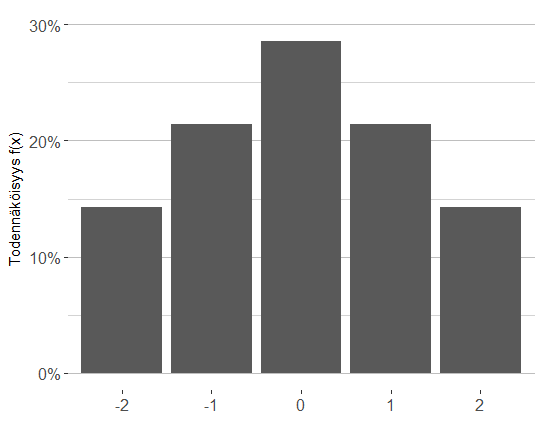
\includegraphics[height = 8cm]{var_a.png}
\captionof{figure}{Expected Value 0, Variance 1.69. (Y-axis represents the values of the pmf.)}
\end{center}

\begin{center}
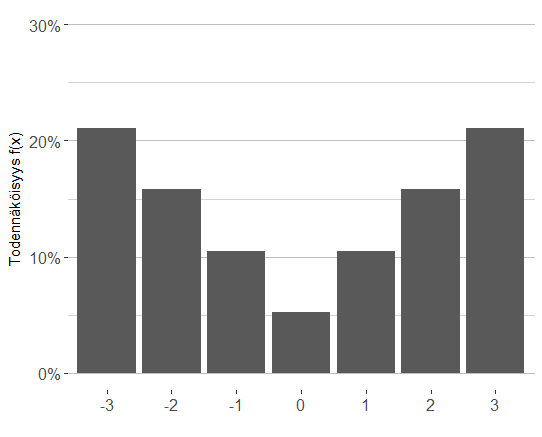
\includegraphics[height = 8cm]{var_b.png}
\captionof{figure}{Expected Value 0, Variance 5.56. (Y-axis represents the values of the pmf.)}
\end{center}

\section{Independence of Random Variables}

\emph{In this section we generalize the concept of independence from events to random variables. Useful stuff.}

Let us take a moment to remember the section \ref{independence}, where we discussed the concept of independence. It turns out that the notion of independence can be utilized in the world of random variables, just as it was possible to define the concept of independent events, each event having its correspondent probability. Intuitively, the independence of random variables mean that their values are not affecting each other: if we know the value of the first random variable, it will not affect on our judgement about the possible value of the second. As it happens, the independence for random variables is defined with the help of independent events:

\begin{maar}
\emph{Independence of Random Variables}. \index{Random Variable!Independence} \index{Independence!of a Random Variable} The random variables $X$ and $Y$ are independent, if 
\[
P((X \in A) \cap (Y \in B)) = P(X \in A) P(Y \in B),
\]
that is, if
\[
\{X \in A\} \independent \{Y \in B\}
\]
for each (smooth enough) sets $A,B \subseteq \R$. In such case we notate
\[
X \independent Y.
\] 
\end{maar}

\begin{remark}
If $X \independent Y$ and $P(Y \in B) > 0$, then the conditional probabilities of the sets are transformed back into unconditional probabilities\footnote{Compare with theorem \ref{lause:conditional_prob}.}:
\[
\begin{split}
P((X \in A) | (Y \in B)) &= \frac{P((X \in A) \cap P(Y \in B))}{P(Y \in B)} \\
 & = \frac{P(X \in A)P(Y \in B)}{P(Y \in B)} \\
 &= P(X \in A).
\end{split}
\]	
\end{remark}

An interesting and useful property is that if random variables are independent, then so are their \emph{transformations}\footnote{With a transformation we mean a random variable, which is derived as a function of some other random variable. For example, a simple transformation of $X$ could be $X^2$. These concepts are discussed further later.}:

\begin{lause}
\emph{Independence of Transformations of Random Variables}. \index{Independence!Transformation of Random Variable} If $X \independent Y$, then for all (smooth enough) functions $g,h : \R \rightarrow \R$ apply that
\[
g(X) \independent  h(Y).
\]
\end{lause}

The concept of independence can be generalized to cover multiple random variables in a following way:
\begin{maar}
\emph{Independence of Multiple Random Variables.} \index{Independence!Multiple Random Variables} A collection of random variables $X_1, \dots, X_n$ is independent, if
\[
P\left(\bigcap_{i=1}^n (X_i \in B_i) \right) = \prod_{i=1}^n P(X_i \in B_i)
\]
for all (smooth enough) sets $B_1, \dots , B_n$. In such case we notate 
\[
X_1, \dots , X_n \independent.
\]
\end{maar}

Often the concept of independence of multiple random variables is useful, for example in the art of statistical analysis, where a single phenomena can have multiple explanatory variables and we would be interested in the respective dependencies of these variables. This, too, is discussed further in later courses. Before moving to the world of continuity, let us practice with few exercises:

\section{Exercises}

\begin{enumerate}
\item A random variable $X$ follows a uniform distribution over a set $\{3, 4, \ldots, 11\}$. Calculate $E(X)$.
\item Infer the distribution of $X$ (name and parameters of the distribution), when
\begin{enumerate}[(a)]
\item $X$ is a number of defective products in a box with 48 products, when the products are considered independent with each product having a probability of 0.5 of being defective.
\item $X$ is the number of aces when picking 13 cards from a standard deck without replacement.
\item In tossing two dice, $X$ is the number of tosses before the first pair of sixes.
\item In a population of 100, $X$ is the amount of colour-blind persons in a 10 person sample, if the population has a total of three colour-blind persons.
\end{enumerate}
\item The random variable $X$ follows a geometric distribution with a parameter $p \in (0,1)$. Show using the definition of expected value and the pmf, that $E(X) = \frac{1-p}{p}$
\item Ever-so-forgetful Mister H has $n$ keys in his key-ring: only one fits the lock in his door, and Mister H has no idea which key it was. Let $X$ be the order number of try which unlocks the door. Calculate the pmf and cumulative density function of $X$, given that Mister H chooses the keys randomly and
\begin{enumerate}[(a)]
\item remembers the keys he has tried,
\item does not remember the keys he has tried.
\end{enumerate}
\item A ferry moves across the lake from coast A to coast B in 10 minute intervals with a capacity of 8 cars. Let us assume, that there are no cars left in the coast A after the ferry leaves. Let us assume further, that within the next 10 minutes, the amount of cars arriving to coast A follows a Poisson distribution with the expected value of 5. What is the probability that the ferry will be full the next time it loads cars from the coast A?
\item Grandparents send their grandchild two gifts with values of 100 euro and 150 euro, respectively. Recently there has been trouble with the postal office, and the probability of losing a package in mail is $0.05$. The grandparents wonder whether they should send the packages in a single parcel, or with two separate ones. Do the math for them according to the following criteria:
\begin{enumerate}[(a)]
\item the expected value of a loss from a lost parcel,
\item the probability of the grandchild getting both of the gifts,
\item the probability of the grandchild getting at least one of the gifts.
\end{enumerate}
\item Persons A, B and C toss a die subsequently while taking turns. Their order is A, B, C, A, B, C\ldots, until one of them tosses a six and wins the game. Calculate the victory probability for each of the players.
\item An ordinary die is tossed four times. Let $X$ be the largest outcome of these tosses. Calculate $E(X)$.
\end{enumerate}

%%%%%%%%%%%%%%%%%%%%%%%%%%%%%%%%%%%%%%%%%%%%%%%%%%%%%%%%%%%%%%%%%%%%%%%%%%%%%%%

\chapter{Continuous Random Variables}\label{cont_rv}

In the previous chapter we introduced the concept of random variable and examined the special case of discrete random variables more closely. In this chapter we expand the notion and move on to discuss \emph{continuous} random variables. The difference between continuous random variables and their discrete counterparts is simple: in the case of continuous random variables, the elements of the value set can not be listed -- the value set is uncountable. This difference forces us to define many key concepts of random variables differently for continuous random variables. For example, the concept of expected value is defined differently although the intuitive concept stays exactly the same.

If the value set of a random variable is uncountable, for example the sets $\R$ or $[0,1]$, we can not use the probability mass function to determine a distribution. In fact, it turns out that in the case of continuous random variables, the probabilities for a given single point is always zero.

In a continuous world, the concept resembling its discrete counterpart, probability mass function, is known as \emph{probability density function}. Instead of summing the probabilities of each individual outcome forming an event, the probabilities for the subsets of sample spaces are obtained with integrating the probability density function. Before venturing any deeper, let us now define these concepts.

\begin{maar}
\label{maar:cont_rv}
\emph{Continuous Random Variable and Probability Density Function\emph{Often abbreviated as PDF. In addition, bear in mind that the concept of continuous random variable is defined through the integral within this definition.}.}\index{Probability Density Function} \index{Distribution!Probability Density}\index{Random Variable!Continuous} \index{Continuous Random Variable} Random variable $X$ has a continuous distribution with a probability density function $f$, if 
\[
P(a \leq X \leq b) = \int_a^b f(x)\dif{x}
\]
for all $a,b \in \R, a<b$.\footnote{In fact, this definition could be generalized from the interval $(a,b)$ to cover all measurable sets $B$, for which $P(X \in B) = \int_B f(x)\dif{x}$.}
\end{maar}

This means, that in the case of a continuous distribution, the probabilities $P(X \in [a,b])$ for for some interval $[a,b]$ can be acquired  as integrating the probability density function over the interval. As with the probability mass function, the probability density function has to be non-negative and its integral has to be $1$ across the whole real axis $\R$. In addition, every function satisfying these properties is also a probability density distribution for some continuous random variable:

\begin{lause}
Properties of a Probability Density Function. Function $f: \R \rightarrow \R$ is a density function for some continuous random variable $X$, if and only if
\begin{enumerate}[(i)]
\item $f(x) \geq 0 \quad \text{for all} \quad x \in \R$,
\item $f$ is integrable over the real axis $\R$ and  
\[
\int_{-\infty}^\infty f(x)\dif{x} = 1.
\]
\end{enumerate}
\end{lause}
\begin{proof}
Left as an exercise.
\end{proof}

Let us next examine an example regarding continuous distributions.

\begin{esim}\label{esim:cont_rv1} 
Uniform distribution and exponential distribution.
\begin{enumerate}[(i)]
\item The Metro arrives at a station in a five-minute interval. A student arrives at the metro station randomly (and does not know when the last metro departed). What is the probability for the student to wait over $3.5$ minutes?

Let us model the waiting time with random variable $X$. Since the metro has an equal chance to arrive anywhere between student's arrival time and $5$ minutes, $X$ follows a \emph{uniform distribution}\footnote{See section \ref{cont_uniform_distr}.} with probability density function
\[
f(x) = \frac{1}{5}.
\] 
Let us now utilize the definition \ref{maar:cont_rv} and calculate the probability for the event where the student has to wait over $3.5$ minutes:
\[
P(3.5 \leq X \leq 5) = \int_{3.5}^5 \frac{1}{5}\dif{x} = \sijoitus{3.5}{5} \frac{x}{5} = \frac{5}{5} - \frac{7}{10} = \frac{3}{10}. 
\]

A major difference and an upside to the discrete counterpart is that now we are able to model the arrival time arbitrarily accurately, and not only for example with one-minute or one-second intervals. We could, for example calculate the probability for the student to wait less than $0.3333\ldots$ minutes.

As with probability mass functions, the probability density functions are also illustrated with graphs. Below is a graph for a uniform distribution between $[0,5]$. The graphical illustration for the metro example can be acquired by highlighting the area below the graph on the interval $[3.5,5]$ -- then the size of the highlighted area is exactly $\frac{3}{10}$.

\begin{center}
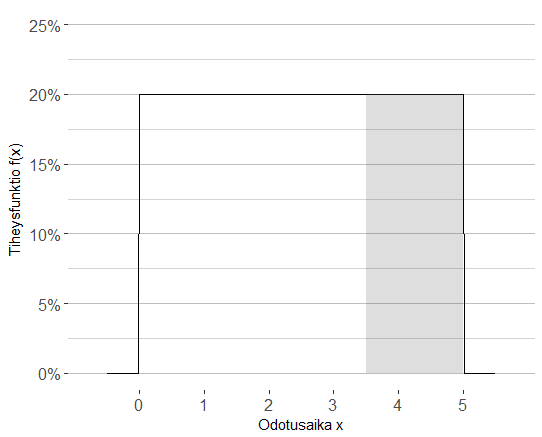
\includegraphics[height = 9cm]{metro.png}
\captionof{figure}{Graph of a random variable $X$ following a uniform distribution (X-axis represents the waiting time, Y-axis the density).}
\end{center}

\item A car is driving on a road, where an insect will smash into the windshield approximately every $0.7$ kilometers. What is the probability for an event that the next insect will hit the windshield within the next two kilometers?

Let us model the length of the road between the insect hits with a random variable $Z$. Now we can assume that $Z$ follows the \emph{exponential distribution}\footnote{See section \ref{exponential_distr}.} with probability density function of  
\[
f(z) = 0.7 e^{-0.7z}.
\]
Now we are able to solve the wanted probability as
\[
P(Z \leq 2) = \int_0^2 0.7 e^{-0.7z}\dif{z} = \sijoitus{0}{2} -e^{-0.7z} = -e^{-1.4} - -e^0 \approx 0.75
\]

Let us illustrate this distribution with a graph, as we did with the uniform distribution.

\begin{center}
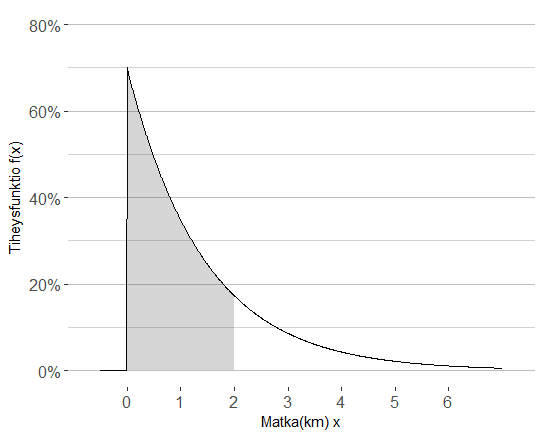
\includegraphics[height = 9cm]{auto.png}
\captionof{figure}{Graph of $Z$ following the exponential distribution (X-axis represent the kilometers until next hit, Y-axis the density).}
\end{center}
\end{enumerate}
\end{esim}

Continuous distributions are often handled with the help of cumulative density function introduced in the previous chapter. The cumulative density function for continuous distributions works exactly as it does with discrete random variables. The cumulative density function was defined for all real-valued $x \in \R$, and the definition tells the amount of ''probability mass'' below the point $x$ -- that is, what is the probability that the random variable $X$ attains a value which is at highest the value $x$.

We can also remember that according to the definition \ref{maar:cdf},
the cumulative density function is $F(x) = P(X \leq x)$ for all $ x \in \R$ for some random variable $X$. For discrete distributions, the cumulative density function is obtained by summing the values of probability mass functions in each point $x$, and respectively the cumulative density functions for the continuous random variables are obtained with integrating the probability density functions\footnote{Notice that this also means that the probability density functions are obtained by differentiating the respective cumulative density functions.}:

\begin{lause}
Cumulative Density Function for a Continuous Random Variable. \index{Cumulative Density Function!Continuous} For a continuous random variable $X$ with a probability density function $f$, the following holds:
\begin{enumerate}[(i)]
\item Cumulative density function $F$ is obtained by differentiating the probability density function:
\[
F(x) = P(X \leq x) = \int_{-\infty}^x f(t)\dif{t} \quad \text{for all} \quad x \in \R.
\] 
\item Additionally, for $f$ 
\[
f(x) = F'(x) 
\]
in each continuity point of $f$.
\end{enumerate}
\end{lause}

The following theorem points out, that for a continuous distribution, the probabilities for each \emph{point} are zero. This notion is useful when remembering whether an examined interval has the outer points included or not: the probabilities are equal for both open and closed intervals.

\begin{lause}
\label{lause:pmf0}
Probabilities for Points in a Continuous Distribution. For a continuous random variable $X$ with a probability density function $f$, the following holds:
\begin{enumerate}[(i)]
\item $P(X = x) = 0$ for all $x \in \R$,
\item $P(a < X < b) = P(a < X \leq b) = P(a \leq X < b) = P(a \leq X \leq b)$ for all $a<b$. 
\end{enumerate}
\end{lause}

\begin{proof}
The first part is directly implied by the definition of a random variable -- let $a=x$ and let $b$ approach $x$ from right. The second part is implied by the first part, together with the additive property of probabilities.
\end{proof}

\begin{remark}
For all $a<b$ an event that a continuous random variable $X$ is smaller or equal to $b$ can be represented as an union of separate events:
\[
(X \leq b) = (X < a) \cup (a \leq X \leq b).
\]
Thus, according to the additive property of probabilities and theorem \ref{lause:pmf0},
\[
\begin{split}
P(a \leq X \leq b) &= P(X \leq b)- P(X < a) \\
				     &= P(X \leq b)- P(X \leq a) \\
				     &= F(b) - F(a).
\end{split}
\]
\end{remark} 

The probabilities for an interval can be thus represented as a subtraction of the values of the cumulative density functions in the outer points of the intervals. If we take a moment to remember the example \ref{esim:cont_rv1}, we notice that when differentiating the probability density function, we actually managed to calculate values for the cumulative density function.

\section{Continuous Distributions}

\emph{In this section we go over the most usual, well-known and practical continuous distributions, and introduce their probability density functions, cumulative density functions and throw in a few examples, too! This section also works as a cheat-sheet for these distributions.}

\subsection{Continuous Uniform Distribution}\label{cont_uniform_distr}

\begin{maar}
Random variable $X$ follows a \emph{(continuous) uniform distribution}\index{Distribution!Continuous Uniform}\index{Continuous Uniform Distribution} over an interval $(a,b)$, if it has a probability density function 
\[
f(x) = \frac{1}{b-a} \quad \text{for each} \quad x \in (a,b),
\] 
and $f(x)=0$ whenever $x \leq a$ or $x \geq b$. In this case, we notate $X \sim \text{Uni}(a,b).$
\end{maar}

The cumulative density function can be acquired by differentiating the probability density function. When $x \in (a,b)$, then
\[
F(x) = \int_{-\infty}^x f(t) \dif{t} = \int_a^x \frac{1}{b-a} \dif{t} = \frac{x-a}{b-a}.
\]

Thus the cumulative density function for a uniformly distributed random variable is
\[
F(x)= \begin{cases}
0, &\text{when} \quad x \leq a \\
\frac{x-a}{b-a}, &\text{when} \quad a < x < b \\
1, &\text{when} \quad  x\geq b. 
\end{cases} 
\]

\begin{esim}
Let us generate a random number from the interval $(0,1000)$. What is the probability that the number generated is between $[500.00,600.00]$?

We can assume\footnote{Note that the number generators are not necessarily random in the same sense as it was an outcome of some random experiment. Most of the random generators generate numbers in a deterministic way, based on parameters that create the illusion of randomness -- for example, a transformation of milliseconds on a current local time.} that the generated number is random, and that the generator is working as intended. Now all numbers in the interval are equally likely, and thus we can mode the situation with random variable $X\sim \text{Uni}(0,1000)$. The probability in question can be calculated as a subtraction of the respective cumulative density functions:
\[
P(500.00 \leq X \leq 600.00) = F(600.00) - F(500.00) = \frac{600}{1000} - \frac{500}{1000} = \frac{1}{10}.
\]
\end{esim}

\subsection{Exponential Distribution}\label{exponential_distr}

\begin{maar}
Random variable $X$ follows an \emph{exponential distribution}\index{Distribution!Exponential} \index{Exponential Distribution} with parameter $\lambda > 0$, if it has a continuous distribution with a probability density function 
\[
f(x) = \lambda e^{-\lambda x} \quad \text{for each} \quad x > 0.
\]
In such case we notate $X \sim \text{Exp}(\lambda)$.

As with the uniform distribution, we are able to acquire the cumulative density function by integrating the pdf:
\[
F(x) = \int_{-\infty}^x f(t)\dif t = \int_0^x \lambda e^{-\lambda t}\dif t = - \sijoitus{0}{x} e^{-\lambda t} = 1- e^{-\lambda x},
\]
when $x>0$ and elsewhere $0$.

\end{maar}

If the occurrence probability of an event for each time interval or for each distance unit is constant, and the events occur independently, the time or the distance between the two occurrences can be modelled as a random variable following an exponential distribution. Moreover, if the amount of events in a time interval follows a Poisson distribution, then the time between each independent event follow an exponential distribution.\footnote{A process, which distributes random events, is called a Poisson Process, if the amount of random events in a time interval follows a Poisson distribution and the time between these events follows an exponential distribution.} We examined this kind of situation briefly in the example \ref{esim:cont_rv1}.

To paraphrase, with exponential distribution we model waiting time or distance between independent events, which have a constant rate of occurrence. For example, following random variables follow the exponential distribution:
\begin{itemize}
\item Time until the next goal in a football match,
\item The distances between road crashes in a given road,
\item Time until the next fish lured up by the fisherman.
\end{itemize}

\begin{esim}
\label{esim:lamp1}
Let us assume, that the burning time of a light bulb follows an exponential distribution with a parameter $\lambda = 0.001$. What is the probability that the bulb burns for over $2000$ hours?

Let us notate the burning time of a bulb with a random variable $X$, and now $X \sim \text{Exp}(0.001)$. The probability in question can be calculated using the probability of a complement;
\[
P(X > 2000) = 1 - P(X \leq 2000) = 1 - F(2000) = e^{-2} \approx 0.135.
\]
We can achieve the same result by directly integrating the probability density function
\[
P(X > 2000) = \int_{2000}^\infty \lambda e^{-\lambda t} \dif t =- \sijoitus{2000}{\infty} e^{-\lambda t} = e^{-2000\lambda } = e^{-2}.
\]
\end{esim}

\begin{remark}
Exponential distribution has this very useful property known as the ''memory loss property'':
\[
P(X > t + h \quad | \quad X > t) = P(X > h).
\]
That is, if we have machine with a lifetime that is exponentially distributed random variable, the probability that the machine works in $h$ moments does \emph{not} depend on the observation time $t$: the probability of the machine working the next day (when observed today) stays constant across each day. 
This means, just to avoid confusion: if observed at $t=0$, the probability for the machine breaking before $t=1$ is equal to the probability of the machine breaking before time $t=6$ when observed at $t=5$ (note that the time distance is equal, $6-5=1-0=1$, in these cases). However, the probability of the machine breaking before $t=6$ when observed at $t=0$ is, of course, different.
\end{remark}

\subsection{Normal Distribution}

\begin{maar}
A continuous random variable $X$ follows a \emph{normal distribution} \index{Distribution!Normal}\index{Normal Distribution} with parameters $\mu \in \R$ and $\sigma^2 > 0$, if its probability density function is
\[
f(x) = \frac{1}{\sqrt{2\pi \sigma^2}} e^{-\frac{(x-\mu)^2}{2\sigma^2}}.
\]
In such case we notate $X \sim N(\mu, \sigma^2)$.
\end{maar}

The parameters of a normal distribution tell the ''location'' and the ''width'' of the distribution. These parameters are often referred to as the \emph{mean parameter} and the \emph{variance parameter}, respectively\footnote{The names of the parameters make sense when thought through the definitions of mean and variance -- mean, or the expected value, means the ''average'' value for the distribution while variance means how much the values of the distribution deviate from its mean. It is easy to see, at least after you've read the next chapter, how variance could be interpreted as the ''width'' of a distribution.}.

If random variable $X$ follows a distribution $N(0,1)$ -- that is, a normal distribution with parameters $\mu=0$ and $\sigma^2=1$, we say that $X$ follows a \emph{standard normal distribution}. In such case the probability density function of $X$ is simplified into
\[
f(x) = \frac{1}{\sqrt{2\pi}} e^{-\frac{x^2}{2}}.
\]

\begin{remark}
\label{remark:norm}
It is important to notice that the random variable $X \sim N(\mu, \sigma^2)$ can always be transformed into a random variable following a standard normal distribution by subtracting it by the mean $\mu$ and dividing it by the deviation $\sigma$. Then, for the random variable
\[
Z = \frac{X-\mu}{\sigma}
\]
holds that $Z \sim N(0,1)$. This specific transformation is called \emph{standardisation}.
\end{remark}

Let us next illustrate, how the probabilities of standard normal distribution are calculated with the help of standardisation.

\begin{esim} \label{esim:norm_stand}
In a certain population, the height of a male population can be modelled with a random variable following a normal distribution with parameters $\mu = 178$ and $\sigma^2 = 25$ (cm). Let us model the male height in said population with $X$. What is the probability that a randomly picked male is between $168$ and $188$ cm in height? How about the probability that the randomly picked male is over $190$ cm tall?

\begin{enumerate}[(a)]
\item Let us solve the probability $P(168 \leq X \leq 188)$ by standardising the random variable $X$ -- subtract the mean parameter and divide by the deviation:
\[
\begin{split}
P(168 \leq X \leq 188) &= P\Big(\frac{168 - 178}{5} \leq \frac{X - 178}{5} \leq \frac{188 - 178}{5}\Big)  \\
&= P(-2 \leq Z \leq 2) \\
&=\Phi (2) - \Phi (-2) =  \\
&=\Phi(2) - (1- \Phi(2)) \\
&= 2 \Phi(2) - 1 = 2 \cdot 0.9772499\ldots -1 \\
&\approx 0.954. \\									  					  
\end{split}
\]
With symbol $\Phi$ we denote the cumulative density function of a standard normal distribution. We are not able to calculate a closed form for this cdf\footnote{The integration gets tricky if solving the problem analytically, which is why we have to resort to numerical solutions.}, and the values for $\Phi$ can be for example calculated with the function \verb|pnorm()| in the R-software, or look the approximate values up from charts found in various literature (see the end of this material, as well!).  
\item As in the previous part:
\[
\begin{split}
P(190 < X ) &= 1 - P(X \leq 190) = P\Big(\frac{X - 178}{5} \leq \frac{190 - 178}{5}\Big)  \\
&= 1 - P( Z \leq 2.4) = 1 - \Phi (2.4) =  1 - 0.9918025\ldots\\
&\approx 0.008. \\									  					  
\end{split}
\]
\end{enumerate}
\begin{center}
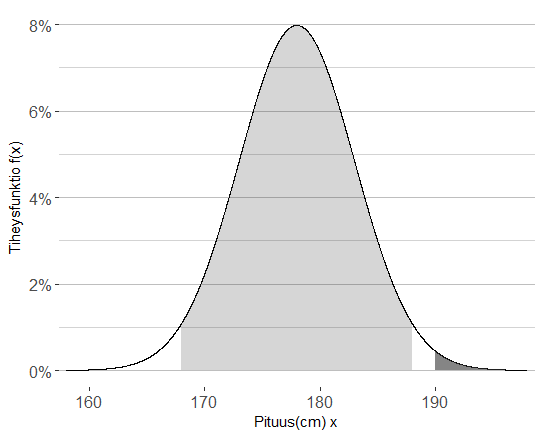
\includegraphics[height = 9cm]{pituus.png}
\captionof{figure}{Normally distributed random variable. The situation in (a) is shaded with light grey and in (b) with dark grey (X-axis represents the height and Y-axis the density).}
\end{center}
\end{esim}

The role of normal distribution in statistics is central. The central role is easily justified, since it turns out that the distribution of the sum of independent random variables approaches normal distribution when the sample size grows. This theorem is known as the \emph{central limit theorem} and we will be discussing it in-depth later on. Also do note that the theorem also holds for the mean of independent random variables.\footnote{Note that you do not need to worry at this point that what ''distribution of random variable approaches some other distribution'' means at this point -- before venturing too deep into these \emph{asymptotic} properties of random variables, I could carefully provide an intuitive explanation that a probability density function, given some sample size $n$, converges into some target pdf. More of this later on.}
 
\section{Expected Value of a Continuous Random Variable}

\emph{In this section we define the concept of expected value for continuous random variables.}

Let us take a short moment to remember that the expected value can be thought as a ''long-term'' average of values the random variable attains. The definition of expected value defined in the last chapter is only defined for discrete random variables: it would make sense that the world of continuous random variables required such an important definition, as well.

\begin{maar}
\emph{Expected Value for a Continuous Random Variable.} \index{Expected Value!For Continuous R.V.} Let $X$ be a continuous random variable with a probability density function $f$. Its expected value is then 
\[
E(X) = \int_{-\infty}^\infty x f(x) \dif x,
\]
if the integral in question converges in absolutely -- that is,
\[
\int_{-\infty}^\infty |x| f(x) \dif x < \infty.
\]
If the integral is not absolutely convergent, then we say that $X$ has no expected value, or that the expected value does not exist.
\end{maar}

Let us next present some examples regarding our newly defined expectation.

\begin{esim}
Let $X$ be a random variable following a uniform distribution $\text{Uni}(a,b)$. Now the expected value of $X$ is
\[ 
E(X) = \int_{-\infty}^\infty x f(x) \dif x = \int_a^b x \frac{1}{b-a} \dif x = \frac{1}{2(b-a)}\sijoitus{a}{b} x^2 = \frac{1}{2}(a+b).
\]
We see that the expected value for a random variable following a uniform distribution on interval $(a,b)$ is the half-point of the interval -- the average of both outer points. This remark lines well with the interpretation of the expected value being the balancing point in a evenly distributed mass, which the uniform distribution represents.
\end{esim}

\begin{esim}
\label{esim:bulb2}
Let us assume that the burning time of a light bulb is represented by a random variable $X$, and that it follows an exponential distribution with parameter $\lambda = 0.001$, -- that is, $X \sim \text{Exp}(0.001)$. What is the expected value of the burning time?

Let us first calculate the general expected value of exponential distribution, using a so-called integration by parts:
\[
\begin{split}
E(X) &= \int_{-\infty}^\infty x f(x) \dif x = \int_0^\infty x \lambda e^{-\lambda x} \dif x \\
	   &= \sijoitus{0}{\infty} x(-e^{-\lambda x}) - \int_0^\infty 1 \cdot  (-e^{-\lambda x}) \dif x \\
	   &= 0 - \frac{1}{\lambda}\sijoitus{0}{\infty} e^{-\lambda x} = \frac{1}{\lambda}.
\end{split}
\]
Now the expected value of the burning time is $E(X) = \frac{1}{\lambda} = 1000$ hours.
\end{esim}

\bigskip

In the past few chapters we have examined and discussed both discrete and continuous random variables, together with their respective differences. Many of the most applied distributions are often either continuous or discrete, but there are also random variables which are neither continuous nor discrete. We will explore this notion in the following remark.

\begin{remark}
The distribution of a random variable doesn't have to be either discrete or continuous. Rather, a random variable can also follow a so-called \emph{mixed distribution}, where the distribution is partially discrete and partially continuous. An example of such distribution could be a burning time of a bulb, if we assumed that the burning time is exponentially distributed random variable with parameter $0.001$, and if we additionally assumed that one tenth of the bulbs are broken with their burning time being $0$. The cumulative density function of such distribution is 
\[
F(x) = \begin{cases}
0, &\text{when} \quad x < 0 \\
\frac{1}{10}, & \text{when} \quad x=0  \\
\frac{1}{10} + \frac{9}{10}(1 - e^{-0.001 x}), &\text{when} \quad  x > 0. 
\end{cases}
\]
\end{remark}

\section{Transformation of a Random Variable}\label{prelim_trans}

By transformation of a random variable we mean a random variable, which is acquired as a result of some function taking random variables as arguments. This sentence is written more formally and clearly in a following theorem:

\begin{lause} \label{lause:prelim_trans}
Transformation of a Random Variable. \index{Transformation} \index{Random Variable!Transformation} If $g :\mathbb{R} \rightarrow \mathbb{R}$ is a function and $X$ is a random variable, then $Y =g(X)$ is also a random variable. 
\end{lause}

In the previous theorem, by simplified notation $Y =g(X)$ we mean that $Y(\omega) = g(X(\omega))$, where $\omega \in \Omega$. That is, $Y$ is a function composition $(g \circ X) (\omega)$.

In fact, we have already examined transformations of random variables in this chapter, more specifically regarding normal distribution. In the example \ref{esim:norm_stand}, we acquired a standardised transformation $Z$ from $X$ with a help of function $\frac{x-178}{5}$, and then inferred that $Z \sim N(0,1)$. An example of a simpler transformation of $X$ could be $Z_2 = 2X$ or $Z_3 = \sqrt{X}$, which, unfortunately do not follow a standard normal distribution. 

Later on, in chapter \ref{rv_trans}, we will examine the properties of transformations more closely -- how their probability mass functions, probability density functions or cumulative density functions are calculated. For now, it is enough that the reader has heard of the concept of transformation and vaguely understand its meaning.

\section{Exercises}
\begin{enumerate}
\item A commute train should arrive in Helsinki at $13.03$ (24h clock). The delay of this train is a random variable, which is uniformly distributed on the interval $(-2,8)$ (minutes). Calculate the probabilities for the train to
\begin{enumerate}[(a)]
\item arrive on time,
\item arrive later than 13:05:20,
\item arrive no later than $1.5$ minutes late.  
\end{enumerate}
\item Derive $E(X)$, when $X$ follows a continuous distribution with a probability density function $f$, where
\begin{enumerate}[(a)]
\item $f(x) = \frac{1}{2}e^{|-x|}$ \quad, where $x \in \mathbb{R}$,
\item $f(x) = \frac{8}{x^3}$ \quad, where $x > 2$,
\item $f(x) = xe^{-\frac{1}{2}x^2}$ \quad, where $x > 0$.
\end{enumerate}
\item The yearly rain amount in Helsinki follows a normal distribution with parameters $\mu = 655$ and $\sigma^2 = 900$ (mm). Calculate a probability for the rain to exceed $800$ mm next year.
\item A continuous random variable $X$ has a probability density function $f(x) = C \cos(x)$, when $\frac{-\pi}{2} \leq x \leq \frac{\pi}{2}$, and $f(x)=0$ elsewhere.
\begin{enumerate}[(a)]
\item Derive the value of constant $C$.
\item Calculate $P(X < 1)$.
\end{enumerate}
\item A factory produces refrigerators, which last a random amount of time in use: the time follows a distribution $Exp(\lambda)$. The parameter $\lambda$ can be altered in the producing process. What should the value of  $\lambda$ be, if we wanted that the probability for the refrigerators to last no more than 5 years would  be no less than $0.5$?
\end{enumerate}

%%%%%%%%%%%%%%%%%%%%%%%%%%%%%%%%%%%%%%%%%%%%%%%%%%%%%%%%%%%%%%%%%%%%%%%%%%%%%%%

\chapter{Properties of Expected Value}\label{expected_value}

In the previous chapters we have defined the concept of expected value for both discrete and continuous random variables, and also practiced novel examples to calculate these expected values directly. In this chapter, we are going to venture deeper into the properties of expected variables and also illustrate why the concept is so vital. In addition, we are going to explore the concepts of variance and covariance -- variance measures the deviation of a random variable and covariance measures linear dependence between two random variables.

Before the technical details emerge, let us use graphs to illustrate the concepts of distribution, expected value and variance: distribution defines the shape, expectation defines the location and variance defines the width.

\begin{center}
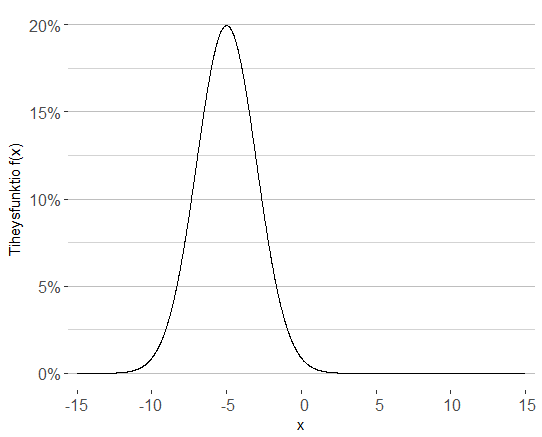
\includegraphics[height = 8cm]{normi1.png}
\captionof{figure}{Probability density function of normally distributed $X$. Expected value $\mu = -5$, variance $\sigma^2 = 2^2 = 4$ (Y-axis: values of pdf).}
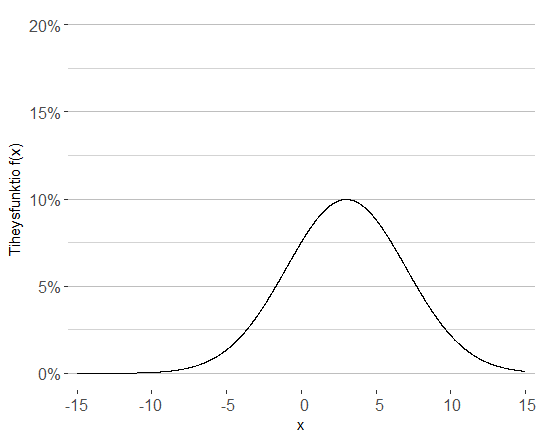
\includegraphics[height = 8cm]{normi2.png}
\captionof{figure}{Probability density function of normally distributed $X$. Expected value $\mu = 3$, variance $\sigma^2 = 4^2 = 16$.}
\end{center}


\section{Expected Value}

\emph{You might have guessed: in this section we explore the properties of expected value.}

As a brief reminder, the expected value of a discrete random variable is defined as the sum 
\[
E(X) = \sum_{i=1}^\infty x_i f(x_i), \text{ where } f \text{ is the pmf of $X$}, 
\]
and the expected value of a continuous random variable is defined as the integral 
\[
E(X) = \int_{-\infty}^\infty x f(x) \dif x, \text{ where } f \text{ is the pdf of $X$,}
\]
if the respective sum and integral converge absolutely. Expected value has the following properties, which hold for both discrete and continuous random variables\footnote{Also notice that while we call a certain statistic of a random variable the expected value, we sometimes refer to the operator $E(\cdot)$ as the \emph{expectation}.}.

\begin{lause}
\label{lause:expected_value_properties}
Properties of Expected Value. \index{Expected Value!Properties} For random variables $X$ and $Y$, and for their expected values, which exist, hold:
\begin{enumerate}[(i)]
\item (Positivity) If $X \geq 0$, then $E(X) \geq 0$.
\item (Linearity) $E(aX + bY) = aE(X) + bE(Y)$ for all $a,b \in \R$.
\item (Monotonicity) If $X \leq Y$\footnote{We say that $X \leq Y$ if $X(\omega) \leq Y(\omega)$ for all $\omega \in \Omega$.}, then $E(X) \leq E(Y)$.
\item If $X \geq 0$ and $E(X) = 0$, then $X$ is a constant $0$ -- that is, $P(X=0) = 1$.
\item If $X$ and $Y$ have the same distribution, then $E(X) = E(Y)$.
\item (Expectation of a constant) In constant $a \in \mathbb{R}$, then $E(a) = a$.
\item If $X \independent Y$, then the expected value of $XY$ is $E(XY) = E(X)E(Y)$.
\end{enumerate}
\begin{proof}
Left as an exercise. Most of the properties are straightforward to proof with the definition of expected value. 
\end{proof}
\end{lause}

Let us now scrutinize the properties of the part $(ii)$ in \ref{lause:expected_value_properties}. Directly from the part $(ii)$ we can derive a crucial theorem, which states that the sums of the expectations equals the expectation of sums, and this property is often called \emph{the linearity of expected value.} Let us now state this in a formal way and afterwards illustrate it in an example.

\begin{lause}\label{lause:expected_value_linearity}
Linearity of Expectation.\index{Expected Value!Linearity} Let $X_1,X_2,\ldots,X_n$ be random variables with finite expected values -- that is, $E(X_i) < \infty$ for all $i = 1, \ldots, n$. Now, the expected value for the sum of these random variables is obtained as the sum of their respective expected values:
\[
E\big(\sum_{i=1}^n X_i \big) = \sum_{i=1}^nE(X_i).
\]
\begin{proof}
Let us use proof by mathematical induction.

When $n = 2$, then according to the part $(ii)$ of theorem \ref{lause:expected_value_properties} we have
\[
E(X_1+X_2) = E(X_1) + E(X_2).
\]

Next, as the induction assumption, let us assume that if $n = k$, then 
\[
E\big(\sum_{i=1}^k X_i \big) = \sum_{i=1}^k E(X_i).
\]

Now let $n = k+1$, from which we derive the induction step as
\[
E\big(\sum_{i=1}^{k+1} X_i \big) = E\big(\sum_{i=1}^{k} X_i + X_{k+1} \big) = \sum_{i=1}^{k} E(X_i) + E(X_{k+1}) = \sum_{i=1}^{k+1} E(X_i),
\]
where the second equality follows from the induction assumption and the part $(ii)$ of \ref{lause:expected_value_properties}.
\end{proof}
\end{lause}

Let us move to the example. In this case, the sample space of the random variable is finite and there are only two random variables -- however, as we just now proved in \ref{lause:expected_value_linearity}, the result is generalized in the domain of multiple random variables, which can also be continuous.

\begin{esim} \label{esim:expected_value_linearity}
A casino offers the following game: with a bet of $10$ euros, the player can toss a coin three times. For each heads, the player wins $5$ euros. In addition, the player can toss a die and if the die results in $6$, the player wins $10$ euros. Is the gamble worth taking?

Let us model the gamble with random variables $X$ and $Y$. Let $X$ be the amount of money won with a single coin toss, and let $Y$ be the amount of money won with a single toss of die. Clearly, according to the definition of expected value, $E(X) = 5 \cdot \frac{1}{2}$ and $E(Y) = 10 \cdot \frac{1}{6}$. Now the expected value of money won in the gamble is according to the linearity of expectation
\[
E(3X+Y) = 3E(X) + E(Y) = 3\cdot \frac{5}{2} + \frac{10}{6}= \frac{45}{6} + \frac{10}{6} = \frac{55}{6}. 
\]
When we subtract the entrance fee from this, we notice that $\frac{55}{6} - 10 = -\frac{5}{6}$, which implies that the expected value of the gamble is negative, and thus not worth playing in a long run.
\end{esim}

For now, we have only examined situations where the expected value truly exists. It is, however, vital to remember that this is not always the case, although the intuitive thought behind expected value not existing can be hard to find. Let us next examine examples with discrete and continuous distributions, which have no expected value.

\begin{esim}
Saint Petersburg Paradox and \emph{Cauchy Distribution}.
\begin{enumerate}[(i)] 
\item Saint Petersburg Paradox\index{Saint Petersburg Paradox}. Let us examine the following game: lets toss a coin until the first heads. The player wins $2^k$ ducat, where $k$ is the number of tosses until the first heads. What would be a reasonable entrance fee for this game?

Let us denote the profit with random variable $X$, which has a value set $\{2,4,8, \dots \}$. Since the probability for getting heads with the $k$th toss is $\frac{1}{2^k}$, the probability mass function of $X$ is now
\[
f(x) = \frac{1}{x} \quad \text{for all} \quad x \in \{2,4,8 \dots\}.
\]
The expected value of the profit is now
\[
E(X) = \sum_{k=1}^\infty x_k f(x_k) =  \sum_{k=1}^\infty 2^k \cdot \frac{1}{2^k} = \sum_{i=1}^\infty 1 = \infty.
\]
That is -- it would be reasonable to pay infinitely ducats for this game\footnote{This obviously does not make any sense, and this example has been used to illustrate the need for a proper \emph{utility theory} examining the perceived utilities of humans.}!

The result is based on the novel fact that the bet is limited, but the profit provided by the casino is, in theory, unlimited and infinite. The 'paradox' can be solved with forcing the casino to limit the maximum  profit attainable.

%Tarkastellaan seuraavaa muunnosta esimerkistä: oletetaan, että kasinon varat (= suurin mahdollinen voittosumma) ovat $2^{20}$ dukaattia (reilu miljoona dukaattia). Kuinka paljon yllä kuvatusta pelistä kannattaa tällöin maksaa?

%Tässä tapauksessa voiton odotusarvo saadaan laskettua geometrisen summan kaavan avulla:
%\[
%\begin{split}
%E(X) &= \sum_{k=1}^{19} 2^k \cdot \frac{1}{2^k} + \sum_{i=20}^\infty 2^{20} \cdot \frac{1}{2^k}\\
% 	 &= 19 +  2^{20} \left(\sum_{k=0}^\infty \frac{1}{2^k} - \sum_{k=0}^{19} \frac{1}{2^k}\right) \\
% 	 &= 19 + 2^{20} \left(2 - \frac{1 - \frac{1}{2}}{1- \frac{1}{2^{20}}}\right) \\
% 	 &= 19 + 2^{20} \frac{\frac{3}{2} - \frac{1}{2^{19}}}{1 - \frac{1}{2^{20}}}
%\end{split}
%\]

\item Cauchy Distribution.\index{Distribution!Cauchy} Random variable $X$ follows a standard Cauchy Distribution, if it has a probability density function of 
\[
f(x) = \frac{1}{\pi} \frac{1}{1 + x^2}\quad \text{for all} \quad x \in \R.
\]
In this case we notate $X\sim \text{Cauchy}(0,1)$. The Cauchy distribution is often used as an example to illustrate a distribution with no finite expected value or variance. For the expected value, this can be shown with integration together with the symmetry of this distribution:
\[
\int_{-\infty}^\infty |x| f(x) \dif x = \frac{1}{\pi} \int_0^\infty \frac{2x}{1+ x^2} \dif x = \sijoitus{0}{\infty} \ln (1 + x^2) = \infty,
\]
\end{enumerate}
\end{esim}

Often we want to consider other \emph{transformations} than sums when discussing expectations. The case of linear transformation was discussed in the example \ref{esim:expected_value_linearity}. Generally, the expected value of a transformation can be thought as a weighted average of the values of the transformation, where the weights are the respective probabilities for the values -- very similar to the case where we discussed the definition of the expected value in the first place: the transformations are random variables, and thus behave similarly. In the case of discrete random variable, the expected value of transformation is obtained as a sum, where the values $g(x)$ are multiplied with their respective probabilities $f(x)$. The case of a continuous random variable behaves similarly, but with integral instead.

\begin{lause}\label{lause:discr_trans_expectation}
Expected Value for a Transformation of Discrete Random Variable. \index{Transformation!Expectation} If $X$ is a discrete random variable with probability mass function $f$, with its value set being $X(\Omega) = \{x_1, x_2, \dots\}$, and $Y = g(x)$ its transformation, then the expected value for random variable $Y$ is
\[
E(Y) = E(g(X)) = \sum_ig(x_i)f(x_i),
\]
if the series converges absolutely. 
\end{lause}

Respectively, this result is analogous for continuous random variables.

\begin{lause}\label{lause:cont_trans_expectation} 
Expected Value for a Transformation of Continuous Random Variable. If $X$ is a continuous random variable with probability density function $f$ and $Y = g(X)$ its transformation, then the expected value for random variable $Y$ is
\[
E(Y) = E(g(X)) = \int_{-\infty}^{\infty}g(x)f(x)\dif x,
\]
if the integral converges absolutely.
\end{lause}
\begin{proof}
Both of the theorems \ref{lause:discr_trans_expectation} and \ref{lause:cont_trans_expectation} are directly proven with the definition of expected value and opening the notation of transformations and finally by showing that the probabilities indicated by $f$, in both cases respectively, stay the same for the corresponding transformed values $g(x)$.
\end{proof}

Let us illustrate these concepts with a following example:

\begin{esim} \label{esim:trans_ev}
Expected values for transformations of both continuous and discrete random variables.
\begin{enumerate}[(i)]
\item In a certain die toss game, the amount of money won is determined through the result of a die toss, in a way that the amount of money won is the result of the toss to the power of two. Is this game worth playing, if the entrance fee is 15 euros?

Let random variable $X$ be the result of the die toss, and now the probability mass function is $f(x) = \frac{1}{6}$ for all $x \in \{1, \ldots, 6\}$. Let random variable $Y$ be the transformation of $X$, such that $Y = X^2$. Now
\[
E(Y) = E(X^2) = \sum_{i=1}^6 i^2 \frac{1}{6} = \frac{91}{6} \approx 15,167.
\]
In other words, the game is profitable in a long run, since the expected value of the money won is larger than the entrance fee.
\item Random variable $X$ follows a continuous uniform distribution on an interval $[0,5]$. Calculate $E(\sqrt{X})$.

The probability density function of $X$ is $f(x) = \frac{1}{5}$. Now
\[
\begin{split}
E(\sqrt{X}) &= \int_{-\infty}^{\infty}\sqrt{x}f(x) = \int_{-\infty}^{0}\sqrt{x} \cdot 0 + \int_{0}^{5}\sqrt{x}\frac{1}{5} + \int_{5}^{\infty}\sqrt{x}\cdot 0 \\
&= \int_{0}^{5}\sqrt{x}\frac{1}{5} = \sijoitus{0}{5}\frac{2x^{3/2}}{15} = \frac{2\cdot\sqrt{5^3}}{15} - \frac{2\cdot\sqrt{0^3}}{15} \\
&\approx 1.49
\end{split}
\]
\end{enumerate}
You can now consider that the transformations in these examples are not linear -- this leads to an observation where $E(g(X))$ and $g(E(X))$ are not equal:
In part $(i)$:
\[
E(X^2) = \frac{91}{6} \neq 3.5^2 = E(X)^2
\]
and in part $(ii)$:
\[
E\big(\sqrt{X}\big) = \frac{2\cdot\sqrt{5^3}}{15} \neq \sqrt{2.5} = \sqrt{E(X)}.
\]
\end{esim}

Now that we know some basic properties for expectations, we are ready to discuss the concepts of variance and standard deviation more thoroughly.

\section{Variance and Standard Distribution}

\emph{In this section we define variance for random variables, and further discuss its properties and examine how to make some calculations regarding variance a bit easier.}

From vast pool of \emph{statistics} regarding distributions, we have so far only examined the expected value. We have noted earlier that the expected value of a distribution represents the location of the distribution or the long-term average of results in some random experiments. A natural extension would be to consider the ''volatility'' of the distribution -- what is the width of the distribution, or how much do the realisations of random variables, on average, differ from the expected value? Variance of the distribution answers to these questions, and now we will discuss the concept of variance and its transformation, standard deviation. 

We define variance as the expected value of the squared difference between the values of random variables and their expectations. Furthermore, we define standard deviation as the square root of variance. Let us now introduce their mathematically sound definitions:

\begin{maar} \label{maar:variance}
\emph{Variance.} \index{Variance} \index{Random Variable!Variance} Let $X$ be a random variable with finite expected value $E(X)$. Now, the variance of $X$ is 
\[
\var (X) = E\left[(X - E(X))^2\right],
\]
if this expected value exists. If $E(X)$ exists, but $E\left[(X - E(X))^2\right] = \infty$, we say that the variance of $X$ is infinite. Other notations for variance include $D^2(X)$ or $\sigma^2$. Sometimes we use the notation $\sigma^2_X$ when handling several random variables simultaneously and we want to specify that the variance in question is the variance of $X$.
\end{maar}

\begin{maar}
\emph{Standard Deviation.}\index{Standard Deviation}\index{Random Variable!Standard Deviation} The square root    
\[
\sqrt{\var(X)}
\]
of $X$'s variance is called its standard deviation. Other notations for standard deviations include $D(X)$, $\sigma$ or $\sigma_X$.
\end{maar}

\begin{remark}
We find it crucial to explain the answer to the question ''why is the variance defined the way it is?''. Earlier, we defined variance as the expected value of the squared difference between the values of random variables and their expectations -- this sounds... complicated, doesn't it? In addition, it would make sense that there would be other ways to measure the ''width'' of a distribution.

The width of a distribution, the average difference between the random variables and their expected values, can be measured also with the standard deviation or simply with $E(|X-E(X)|)$. Why variance is the ''standard'' measurement? To put it simply, variance is defined as it is solely for the reason that it makes mathematics more easy, and variance defined as it is has some wonderful properties -- for example, almost all of the properties introduced in this section hold because variance is defined as above, and they do not necessarily hold for standard deviation or other similar measurements. For example, standard deviation is not linear even when the random variables are independent.
\end{remark}

As you might have noticed, calculating variance directly from the definition \ref{maar:variance} might pose to be difficult in many exercises. It turns out, however, that variance can also be presented with the help of the \emph{second moment\footnote{The moments of random variables can be calculated with so-called moment-generating functions, which are further explored in later courses.}} of a random variable.

\begin{maar}
\emph{Second Moment.} The expected value of the square of a random variable $E(X^2)$ is called its second moment. For a discrete random variable $X$ with probability mass function $f$, it can be calculated as the sum
\[
E(X^2) = \sum_{i=1}^\infty x_i^2f(x_i).
\]
Respectively, for continuous random variable $Y$ with probability density function $g$ the second moment can be calculated as integral
\[
E(Y^2) = \int_{-\infty}^\infty y^2 g(y) \dif y.
\]
\end{maar}

Now, the variance can be calculated with the help of following theorem:

\begin{lause}
\label{lause:variance}
If a second moment $E(X^2)$ exists for random variable $X$, then its variance exists as well, and this variance can be calculated as 
\[
\var(X) = E(X^2) - [E(X)]^2.
\]
\end{lause}

\begin{proof}
The existence and finiteness of expectation follows from the existence of the second moment, since
\[
|x| \leq 1 + x^2 \quad \text{for all} \quad x \in \R.
\]
Now the theorem follows from the linearity of expectation -- that is, from the part $(ii)$ of theorem \ref{lause:expected_value_properties}:
\[
\var (X) = E\left[(X - E(X))^2\right] = E\left[X^2 - 2XE(X) + E(X)^2\right] = E(X^2) - [E(X)]^2.
\]
\end{proof}

\begin{remark}
Be careful with the notations! Often we shorten $[E(X)]^2=E(X)^2$, so bear in mind that you are always aware of which term to square and which term has the squared random variable inside the expectation. In this material, we also use the shorthand notation $E(X)^2$. 
\end{remark}

Let us next consider calculating variance for a continuous, uniformly distributed random variable:

\begin{esim}
Let $X$ be a random variable following uniform distribution on the interval $(a,b)$ -- that is $X \sim \text{Uni}(a,b)$, and additionall the expected value of $X$ is $E(X) = \frac{1}{2}(a+b)$. Let us first calculate the second moment of $X$:
\[
E(X^2) = \int_{-\infty}^\infty x^2 f(x)\dif x = \int_a^b \frac{x^2}{b-a} \dif x= \frac{1}{3(b-a)} \sijoitus{a}{b} x^3 = \frac{b^3 - a^3}{3(b-a)}. 
\] 
Now, the variance can be calculated according to theorem \ref{lause:variance}:
\[
\var(X) = E(X^2) - [E(X)]^2 = \frac{b^3 - a^3}{3(b-a)} - \left[\frac{1}{2}(a+b)\right]^2 = \frac{1}{12}(b-a)^2.
\]
If we had calculated the variance directly from the definition \ref{maar:variance}, we would have ended up with equal result.
\end{esim}

As with expectation, properties for variance prove to be useful. It turns out that variances can be calculated for various transformations of random variables, of which linear transformation is a simple example. The variance of linear transformation can be calculated using the following theorem.

\begin{lause}
Variance of a Linear Transformation.\index{Variance!Linear Transformation} If the variance of random variable $X$ exists and $a,b \in \R$, then
\[
\var(aX + b) = a^2\var(X).
\]
\end{lause}

\begin{proof}
\item According to the linearity of expectation we have $E(aX + b) = aE(X) + b$, and furthermore from the definition of variance we get
\[
\var(aX + b) = E([aX + b - aE(X) - b]^2) = a^2 E([X-E(X)]^2) = a^2 \var(X).
\]
\end{proof}

The previous theorem we noticed that adding a constant into the random variable doesn't change its variance\footnote{Remember from the previous chapters, that adding a constant changes the expected value of a random variable by the same amount.}, but instead multiplying the random variable with a constant squares the effect of the constant. This is intuitive in a sense that variance in fact measures the average \emph{squared} deviation from the expected value.

In the following theorem we present a few properties for variance, which may prove themselves useful.

\begin{lause} \label{lause:var_prop}
Properties of Variance. \index{Variance!Properties} For random variables $X$ and $Y$, which have existing variances, the following hold:
\begin{enumerate}[(i)]
\item $\var(X) \geq 0$
\item If $\var(X) = 0$, then $X$ is a constant.
\item If $X \independent Y$, then $\var(X+Y) = \var(X) + \var(Y)$ 
\end{enumerate}
\end{lause}

\begin{proof}
\rule{0pt}{3ex}
\begin{enumerate}[(i)]
\item Since $(X - E(X))^2 \geq 0$, then $\var(X) \geq 0$, if it exists as a real-valued number.
\item If $\var(X) = 0$, then
\[
P(X = E(X)) = P((X - E(X))^2 = 0) = 1,
\]
from which we infer that $X$ obtains the value $E(X)$ with probability $1$ -- that is, $X$ is a constant.
\item $E(X+Y) = E(X)+E(Y)$, and thus, since the random variables are independent,
\[
\begin{split}
\var(X+Y) &= E((X+Y - (E(X)+E(Y)))^2)\\
&= E[(X-E(X)+Y-E(Y))^2] \\
&= E[(X-E(X))^2+2(X-E(X))(Y-E(Y))+(Y-E(Y))^2] \\
&= E[(X-E(X))^2+(Y-E(Y))^2] + E[2(X-E(X))(Y-E(Y))] \\
&= \var(X) + \var(Y) + 2 \cdot 0 \cdot 0
\end{split}
\]
\end{enumerate}
\end{proof}

It turns out that the part $(iii)$ of the previous theorem -- variance for the sum of two independent random variables -- can be generalized to cover the case of multiple random variables:

\begin{lause}
If random variables $X_1, \dots ,X_n$ are independent -- that is, $X_1, \dots ,X_n \independent$, with their variances being finite, then
\[
\var\left(\sum_{i=1}^n X_i \right) = \sum_{i=1}^n \var(X_i).
\]
\end{lause}

Now that we have covered the basic properties of variance, let us move to the concepts of covariance and correlation -- which measure the dependence between two random variables. Coincidentally, these concepts are closely tied with variance.

\section{Covariance and Correlation}

\emph{In this section we briefly introduce the concepts of covariance and correlation, which measure the linear dependence between two random variables. Since this material doesn't cover multivariate distributions per se, we are trying to simplify some of the discussion.}

The linear dependence between two random variables is measured through their \emph{covariance}. Before accidentally venturing too deep into the discussion, let us first define covariance:

\begin{maar} \label{maar:covariance}
\emph{Covariance.}\index{Covariance} Let $X$ and $Y$ be random variables with expected values $E(X)$ and $E(Y)$, respectively. The covariance between these two random variables is now 
\[
\cov(X,Y) = E([X - E(X)][Y - E(Y)]),
\]
if this expected value exists. It also turns out, that the sufficient condition for the existence of covariance is that the second moments of $X$ and $Y$ are finite.
\end{maar}

From this definition we see, that the definition of covariance closely resembles the definition of variance. For example, what would happen if we calculated the covariance between $X$ and $X$? The following theorem answers to this question, and in addition presents other properties for covariance. Especially the second part tells us, that variance is in fact a special case of covariance: variance of $X$ is the covariance of $X$ between $X$.

\begin{lause}
Properties of Covariance\index{Covariance!Properties}. Let $X$ and $Y$ be random variables with finite second moments. Then
\begin{enumerate}[(i)]
\item $\cov(X,Y) = \cov(Y, X)$,
\item $\var(X) = \cov(X,X)$,
\item $\cov(aX, Y) = a \cov(X,Y)$.
\end{enumerate}
\end{lause}

\begin{proof}
The first and the second part are directly implied by the definition of covariance \ref{maar:covariance}. The third part can be derived from the definition, and is left as an exercise.
\end{proof}

Similarly with variance, we are able to derive the covariance to a form which resembles the second moment theorem of variance. Just as with variance, this form often simplifies calculations:

\begin{lause} \label{lause:covariance}
Let $X$ and $Y$ be random variables with finite second moments. Then
\[
\cov(X,Y) = E(XY) - E(X)E(Y).
\]
\end{lause}

\begin{proof}
Left as an exercise. Hint: you should start by expanding the product inside the expectation in \ref{maar:covariance}.
\end{proof}

\bigskip

Covariance can sometimes be a tricky term to evaluate: as with expected value and variance, covariance can theoretically be extremely large. What would the covariance be, if the two random variables in question had a exact linear dependence? Often, instead of covariance, we use a so-called standardised covariance to present linear dependence between random variables. This standardised covariance is called \emph{correlation}, and it is obtained by dividing the covariance of two random variables with their standard deviations.

\begin{maar}\label{maar:correlation}
\emph{Correlation.} Let $X$ and $Y$ be random variables with their respective expected values and variances being finite. Then, the correlation between $X$ and $Y$ is 
\[
\corr(X,Y) = \frac{\cov(X,Y)}{\sqrt{\var(X)\var(Y)}}.
\]
\end{maar}

It turns out that correlation of two random variables always attains values between $[-1,1]$. If the correlation is $1$, the two random variables have an exact linear relationship, and if the correlation is $-1$, then the exact linear relationship is negative. If the value of correlation is $0$, then there is no \emph{linear} relationship between the two random variables.

This interpretation is further reinforced with the remark that the covariance and correlation between two independent random variables is $0$. The following theorem is a direct implication of the part $(vii)$ of theorem \ref{lause:expected_value_properties}, which tells that the expected value of the product of two independent random variables is obtained as the product of their respective expected values.

\begin{lause}
\label{lause:non-corr}
If random variables $X$ and $Y$ are independent -- that is, $X \independent Y$, then
\[
\cov(X,Y) = 0,
\] 
and also 
\[
\corr(X,Y) = 0.
\]
\end{lause}

\begin{proof}
The proof is fairly straightforward: 
\[
\cov(X,Y) = E(XY) - E(X)E(Y) = E(X)E(Y) - E(X)E(Y) = 0.
\]
\end{proof}

\begin{remark}
If $\cov(X,Y) = 0$, we say that $X$ and $Y$ are \emph{uncorrelated}. According to the previous theorem, uncorrelation always follows the independence of random variables. However, independence does not always follow uncorrelation -- this quirky remark can be explained since correlation and covariance only measure the \emph{linear} relationship and dependence between two random variables. If the relationship between these two random variables is nonlinear, it can not be measured by covariance.

A classical example which highlights this remark is following: let us examine a random variable $X$ following standard normal distribution. Since the probability density function of $X$ is symmetrical with respect to its expected value $0$, we have $E(X) = E(X^3) = 0$. Now, if we examine the covariance between $X$ and its transformation $X^2$, we see that 
\[
\cov(X,X^2) = E(X \cdot X^2) -  E(X)E(X^2) = 0 - 0 = 0,
\]
but of course $X$ and $X^2$ are not independent.
\end{remark}

If two random variables are not independent, their sum can be calculated with the help of their covariance. For subtraction and other linear combinations, a similar theorem can be derived, as well. 

\begin{lause}
If the variances of random variables $X$ and $Y$ are finite, then
\[
\var(X + Y) = \var(X) + \var(Y) + 2\cov(X,Y).
\]
Especially, if $X \independent Y$, then
\[
\var(X + Y) = \var(X) + \var(Y).
\]
\end{lause}

\begin{proof}
The proof is fairly straightforward: first expand the products within the expectations and then abuse the linearity property of expectation:
\[
\begin{split}
\var(X+Y) &= E((X+Y)^2) - E(X+Y)^2 \\
			    &=E(X^2) + 2E(XY) + E(Y^2) - E(X)^2 - 2E(X)E(Y) - E(Y)^2 \\
			    &= \var(X) + \var(Y) + 2 \cov(X,Y).
\end{split}
\]
The second part of the theorem is implied by \ref{lause:non-corr}, which tells us that $\cov(X,Y) = 0$. 
\end{proof}

\bigskip

We have now learned the definitions for variance, covariance and correlation, and in addition have learned about their vital properties. These properties prove themselves useful in the future, and the following example neatly collects multiple useful concepts together. Before this example, we will present the \emph{Cauchy-Schwarz} inequality, which is needed in the example (and elsewhere in the field of probability, as well).

\begin{lause}
\label{lause:cauchy_schwarz}
Cauchyn-Schwarz Inequality. \index{Cauchyn-Schwarz Inequality} For random variables $X$ and $Y$ we have that
\[
|E(XY)| \leq E(|XY|) \leq \sqrt{E(|X|^2)} \sqrt{E(|Y|^2)}.
\]
\end{lause}
\begin{proof}
Omitted.
\end{proof}

Now that we have been introduced this theorem in a fairly deus ex machina style, let us proceed to the example. It could be useful that the student would try to solve this example before reading the solution -- despite the order of trial and error, this example is \emph{important} and should be studied carefully.

\begin{esim}
Let $X$ and $Y$ be random variables with finite variances. Let us show that the following properties are equal -- that is, they all imply each other.
\begin{enumerate}[(i)]
\item $\cov(X,Y) = 0$,
\item $E(XY) = E(X)E(Y)$,
\item $\var(X + Y) = \var(X) + \var(Y)$.
\end{enumerate}

From the existence of $\var(X)$ and $\var(Y)$ it follows, that the expectations $E(X^2)$, $E(Y^2)$, $E(X)$ and $E(Y)$ exist as well. Now, according to Cauchy-Schwarz inequality \ref{lause:cauchy_schwarz}, the expectation $E(XY)$ exists, as well. Now the random variables $X$ and $Y$ have a covariance according to the definition \ref{maar:covariance} and the theorem \ref{lause:covariance}. The covariance is calculated as 
\[
\cov(X, Y) = E[(X-E(X))(Y-E(Y))] = E(XY) - E(X)E(Y).
\]
In addition, the random variable $X+Y$ has a variance
\[
\begin{split}
\var(X+Y) &= E((X+Y)^2) - E(X+Y)^2 = E(X^2+2XY+Y^2) - (E(X)+E(Y))^2 \\
&= E(X^2) + 2E(XY) + E(Y^2) - E(X)^2 -2E(X)E(Y) - E(Y)^2 \\
&= (E(X^2) -E(X)^2) +2(E(XY)-E(X)E(Y)) + (E(Y^2) -E(Y)^2) \\
&= \var(X) + 2\cov(X, Y) + \var(Y).
\end{split}
\]
Now, it can be seen that
\[
\cov(X, Y) = 0 \Leftrightarrow E(XY) - E(X)E(Y) = 0 \Leftrightarrow E(XY) = E(X)E(Y),
\]
that is, the parts $(i)$ and $(ii)$ are equal. In addition, we can show that
\[
\cov(X,Y) = 0 \Leftrightarrow \var(X+Y) = \var(X) + \var(Y),
\]
that is, the parts $(i)$ and $(iii)$ are equal, and thus all of the parts in the example imply each other and thus are equal.

Again, please do note that from none of these conditions follow that $X$ and $Y$ would be independent.
\end{esim}

Now we have studied the basics of the expected value, variance, covariance and correlation. We defined these concepts, discussed their properties and highlighted them with some examples. These concepts are one of the most important concepts within the field of probability, and many of these examples will prove themselves to be useful later on.

\section{Exercises}

\begin{enumerate}
\item The points of a triangle in a flat surface are the origin point and two random points $X$ and $Y$ picked from the x-axis and y-axis, respectively. $X$ and $Y$ are independent random variables, and they follow a normal distribution with parameters $\mu = 0$ and $\sigma^2 = 1$. Derive the expected value of the triangle's surface area.
\item Let $X$, $Y$ and $Z$ be independent random variables, with all of them having the same expected value $\mu$ and variance $\sigma^2$. Derive the expected value and the variance for the following (transformed) random variables:
\begin{enumerate}[(a)]
\item $2X + 3$,
\item $X - Y$,
\item $X - \frac{1}{2}Y$,
\item $X + 2Y + 3Z$,
\item $XY$,
\item $XYZ$.
\end{enumerate}
\item Let $X$ be a random variable which represents the result of an ordinary die toss. Derive $\var(X)$.
\item Let $X$ be a random variable with probability density function $f(x) = 2x$, when $0 \leq x \leq 1$. Derive $\var(X)$. 
\item (Ross Example 7.4a) Let $X_1 \ldots X_n$ be independent and identically distributed random variables with expected value $\mu$ and variance $\sigma^2$, and let $\bar{X} = \sum_{i=1}^n \frac{X_i}{n}$ be their sample mean. What is the variance $\var(\bar{X})$ of the sample mean?
\item Two dice are tossed. Consider two random variables $X$ = ''result of the 1st toss'' and $Y$ = ''the sum of the two results''. Derive $\corr(X, Y)$. 
\end{enumerate}

%%%%%%%%%%%%%%%%%%%%%%%%%%%%%%%%%%%%%%%%%%%%%%%%%%%%%%%%%%%%%%%%%%%%%%%%%%%%%%%

\chapter{Inequalities and Limit Theorems}\label{limit}

Now that we have established the foundations of random variables, distributions and statistics -- the bricks and mortars of the modern day probability theory --, we are finally able to proceed to the most groundbreaking results in the field. Theorems presented in this chapter are not only vital for the advancements of theoretical research\footnote{For example, the Chebyshev's inequality is famous in the art of proving that second moments exist, which is elementary requirement for many theorems, as you by know should have realised. Additionally, both the central limit theorem and the law of large numbers are proved using these inequalities.}, but also in the practical side of probability. An example of the practical side would be the \emph{normal approximation}, which is discussed in the end of this chapter.

This chapter is also the final chapter of the standard material discussed in the elementary level probability course. This chapter uses nearly all information we've acquired so far from this material -- although you might realise that the normal approximation is not as useful as it was before the surge of computing power, as theorem it is certainly interesting, and additionally it sums up the learning goals of this course adequately. 

\section{Inequalities}

\emph{As the name of this section implies, in this section we discuss the famous inequalities of probability. They are useful and might require a moment of thinking before their usage becomes crystal clear. Hang in there!}

Next, we are going to introduce two most fundamental inequalities in probability: Markov's inequality and Chebyshev's inequality\footnote{Note that often the names for these inequalities might be unclear: in some literature Markov's inequality is sometimes referred as Chebyshev's. The romanisation for Chebyshev might also in some literature be T\v{s}eby\v{s}ev.}. With these inequalities we are able to calculate upper limits for the so-called ''tail probabilities'' of random variables -- that is, for probabilities that the values of a random variable deviate from their expected value by at least some constant, even in the unfortunate case that we did not know the probability mass or probability density functions of these random variables.

The fundamental function of mathematical theorems is that the theorems have some assumptions, from which a result is then derived. This result is then ''bookmarked'' as theorem, and is readily applied into problems which satisfy these assumptions. It could be safe to say that if the theorem requires few assumptions and has a strong result, the theorem is good -- assumptions provide information and restrict the menu of possible outcomes. Few assumptions usually lead to very general and not-so-practical results. This piece of information can be used when learning the following inequalities: Markov's inequality assumes only that for a non-negative random variable, its expected value is known. On the other hand, Chebyshev's assumes a little more: it assumes that the variance is also known -- thus it would make sense that since the Chebyshev's theorem requires more assumptions -- the playground is more restricted -- the result would be more accurate, under its assumptions.

As stated, Markov's inequality assumes only that for a non-negative random variable, its expected value is known. Given this assumption, the theorem states that the probability for $X$'s value to be at least as large as some constant $a$ is less than the expected value of $X$ divided by $a$. To prove this inequality, we require so-called characteristic functions of random variables, which are not discussed in this material and thus the proof is omitted.

\begin{lause} Markov's Inequality.\index{Markov's Inequality} If $X$ is a non-negative random variable, $X \geq 0$, and the expected value of $X$ exists, then
\[
P(X \geq a) \leq \frac{E(X)}{a} \quad \text{for all} \quad a > 0.
\]
\end{lause}
\begin{proof}
Omitted.
\end{proof}

%\begin{proof}
%Määritellään satunnaismuuttuja 
%\[
%Y = \mathbf{1}_{[a, \infty)}(X) = \begin{cases}
%1, &\text{kun} \quad X \geq a \\
%0, &\text{muuten}.
%\end{cases}
%\]
%Koska aina $X \geq Y$, lauseen \ref{lause:odotusarvon_omin} kohdan (iii) ja odotusarvon lineaarisuuden nojalla
%\[
%E(X) \geq E(Y)	=  aE(\mathbf{1}_{[a, \infty)}(X)) = a(0 \cdot P\{X < a\} +  1 \cdot P\{X \geq a\}) = aP\{X \geq a\}.
%\]
%Nyt väite seuraa jakamalla epäyhtälön kumpikin puoli $a$:lla.
%\end{proof}

If $\mu = E(X) > 0$, by setting $a=k\mu$ we can rewrite Markov's inequality as 
\[
P(X \geq k\mu) \leq \frac{1}{k} \quad \text{for all} \quad k > 0.
\]
Now, to reiterate, the inequality states that the probability for $X$'s value to be at least as large as $k$ times its expected value $E(X)$ is maller than $1/k$. This form of the inequality also is more easily connected to the Chebyshev's inequality -- due to this connections, these equalities are sometimes referred to as the first moment (Markov) and the second moment (Chebyshev) inequalities.

Chebyshev's inequality can be applied to all random variables, which have known (and finite) expected value and variance. According to this equality, the probability that the values of a random variable deviate at least $k$ standard deviations from the expected value is smaller than $1/k^2$. Again, this might be easier to comprehend after seeing the mathematically sound definition.

\begin{lause}
Chebyshev's Inequality\index{Chebyshev's Inequality} If $X$ is a random variable with existing expected value $\mu = E(X)$ and variance $\sigma^2 = \var(X) > 0$, then
\[
P(|X-\mu| \geq k\sigma ) \leq \frac{1}{k^2} \quad \text{for all} \quad k > 0.
\]
\end{lause}

\begin{proof}
Let us apply the Markov's inequality in this proof, despite the awkward fact that we did not prove it -- bear with us. By using the Markov's inequality for random variable $|X-\mu|^2$ and constant $a = k^2\sigma^2$ together with the definition of variance, we obtain
\[
P(|X-\mu|\geq k\sigma) = P(|X-\mu|^2 \geq k^2\sigma^2) \leq \frac{E(|X - \mu|^2)}{k^2 \sigma^2} = \frac{\sigma^2}{k^2\sigma^2} = \frac{1}{k^2}.
\] 
\end{proof}

Let us next apply the inequalities in an example:

\begin{esim}
Continued from the example \ref{esim:lamp1}. Let us yet again examine lightbulbs, which have a burning time $X$ which follows the exponential distribution with expeced value of $1000$ hours -- that is, $X \sim \text{Exp}(0.001)$. 

Since $X \geq 0$ and the expected value is known, with Markov's inequality we can obtain a probability for the bulb to burn at least $3000$ hours:
\[
P(X \geq 3000) = P(X \geq 3\mu) \leq \frac{1}{3}.
\]
With the art of integration by parts, we can obtain variance for the exponential distribution as $1/\lambda^2$; thus the standard deviation of  $X$ is $\sigma = 1/\lambda = 1000$. Since we now know the variance, we are able to obtain stricter upper limit for the probability via Chebyshev's inequality:
\[
P(X \geq 3000) = P(X-\mu \geq 3000-\mu) \leq P(|X-\mu| \geq 3000-\mu) = P(|X-\mu| \geq 2\sigma) \leq \frac{1}{4}.
\]

Of course, in this example we know the cumulative density function $F$, which means that instead of \emph{approximating} the upper limit, we are able to calculate the exact value for it:
\[
P(X \geq 3000) = 1 - F(3000) = e^{-0.001 \cdot 3000} = e^{-3} \approx 0.05.
\]

To illustrate the example the example further, in the following chart are the upper limits calculated from the inequalities of Markov and Chebyshev, together with the exact values for the tail probabilities of $X$:

\bigskip

\begin{tabular}{l l l L{6cm}}
\toprule
$x$ & Markov & Chebyshev & Exact value of $P(X \geq x)$\\
\midrule
$3000$ & 0.33 & 0.25 & 0.050\\
$4000$ & 0.25 & 0.11 & 0.018\\
$5000$ & 0.20 & 0.0625 & 0.007\\
$10000$ & 0.10 & 0.012 & $4.54 \cdot 10^{-5}$\\
\bottomrule 
\end{tabular}

\bigskip

We notice that the upper limits acquired by the inequalities are kind of rough, and in addition, for large deviations Chebyshev's inequality provides much tighter upper limit than its Markov counterpart -- this is due to the fact that the assumption of variance in Chebyshev's gives us more information.

Even thought the upper limits given by these ineqlualities prove to be quite inaccurate, it is vital to still recognise these inequalities as groundbreaking: we can calculate these upper limits even without knowing the distribution of the random variable. In addition, they both are used in proving the results of central limit theorem and law of large numbers -- results we are going to discuss shortly.
\end{esim}

\section{Limit Theorems}

\emph{The goal of this section is to introduce two very central theorems of probability: the central limit theorem and the law of law numbers. The concept of limits of random variable sequences are somewhat theoretical, but the results itself are extremely useful.}

In the field of probability, there are two major theorems considering sequences $X_1, \dots , X_n$ of independent and identically distributed\footnote{As usual, there are several different versions of these theorems in circulation with different assumptions: we present the classical versions of these theorems, even though the same results can be proven with less assumptions.} random variables\footnote{These kind of sequences have been introduced few times in this material, and often they are referred to as i.i.d sequences.}. Regarding these sequences, we are especially interested in the behaviour of sums or means of random variables, when the random experiment realising the corresponding random variables is repeated infinitely. It turns out that the sequence of means approaches the shared expected value of these random variables, and the distribution of these means approaches normal distribution, with the mean parameter being the shared expected value of the random variables. 

These so-called limit theorems are extremely central in the theory of statistical inference. Sometimes, we are not able to calculate exact distributions for so-called estimators\footnote{By estimator we mean an approximation of a statistic, which is modelled as random. In other words, as we model non-realised random variables as random -- that is, we do not know their value at the point of observation -- we are able to model transformations and combinations of these random variables, most often the sample mean, which is used to \emph{estimate} the distribution mean -- the expected value. When the random variables are realised -- when we have observed the outcome of the random experiment -- this mean is then the \emph{estimate} of the expected value. To reiterate: estimator is the non-realised, random variable version of an estimate. These concepts are further discussed in any statistical inference class.}. In these cases we have to apply the central limit theorem, which states that with ''large enough sample size'', the sums and sample means of independent and identically distributed random variables are approximately normally distributed. However, before exploring the possibilities of the central limit theorem, we have to learn something about the so-called law of large numbers.

\subsection{Law of Large Numbers}\label{sll}

In the early chapters of this material, we explained that one interpretation of expected value is that it is the long-term average profit per game, when this game is repeated many times. This interpretation is based on the one of the most central results in probability, the law of large numbers. According to the law of large numbers, the mean of independent random variables $X_1, \dots X_n$ approaches their shared expected value, when $n$ approaches infinity -- that is, when the random experiment is repeated $n$ times and $n \rightarrow \infty$. Mathematically speaking, as a function of repeated times $n$, the limit of the sequence of is the shared expected value $\mu$ of random variables $X_i$. 

The law of large numbers is also the basis for many scientific experiments: if the sample size is large enough, then we can argue that the average success ratio in an experiment is close to the \emph{actual} success probability. For example, we can test whether a new drug cures some disease -- if the test setting is professional and the statuses of the patients are independent, with large enough sample size, the frequency of cured patients is close to the actual curing probability of the drug.

\bigskip

We have used a lot of terminology regarding limits, convergences and approaching in the beginning of this chapter. Let us define what we mean by convergence in the context of random variable sequences. First, we need to be reminded that a sequence of random variables is indeed a sequence of functions\footnote{Yes, as in \ref{maar:rv}, random variables are functions.} from the sample space to the set of real numbers. The convergence of random variables can be defined in many ways depending how strongly we want them to converge: in the context of this material we use a so-called \emph{stochastic convergence}.

\begin{maar}
\emph{Stochastic Convergence.}\index{Stochastic Convergence} A sequence of random variables $X_1, X_2, \dots$ \emph{stochastically converges} to a limit random variable $X$, if
\[
\lim_{n\rightarrow \infty}P(|X_n - X| \geq \epsilon) = 0 \quad \text{for all} \quad \epsilon > 0.
\]
In such case we notate
\[
X_n \overset{p}{\rightarrow} X.
\]
\end{maar}

Do notice, however, that in the general definition of stochastic convergence, $X$ can be a random variable, although in the next theorem the limit is a constant $\mu = E(X_i)$.

Now, we have enough tools to formulate the law of large numbers and prove it using the Chebyshev inequality. To make the proof easier and manageable for this material, we impose an additional assumption that the random variables $X_1, X_2, \dots$ have shared variance, in addition to the shared expected value.

\begin{lause}
(Weak) Law of Large Numbers, (LNN)\index{Law of Large Numbers} Let $X_1, X_2, \dots$ be a sequence of independent random variables\footnote{Note that we do not require that the random variables follow the same distributions. It is enough that the expected value and the variance are the same for these random variables.} with the same expected value $\mu = E(X_i)$ and the same variance $\sigma^2 = \var(X_i) \leq \infty$. Now, the sequence $\bar{X}_1, \bar{X}_2, \dots$ of average means
\[
\bar{X}_n = \frac{1}{n} \sum_{i=1}^n X_i
\]
stochastically converges to the shared mean of these random variables -- that is,
\[
\bar{X}_n \overset{p}{\rightarrow} \mu,
\]
that is that is, 
\[
\lim_{n\rightarrow \infty}P(|\bar{X}_n - \mu| \geq \epsilon) = 0 \quad \text{for all} \quad \epsilon > 0.
\]
\end{lause}

\begin{proof} 
By the independence of the random variables, the variance of their mean $\bar{X}_n$ is
\[
\var(\bar{X}_n) = \var\left( \frac{1}{n} \sum_{i=1}^n X_i \right) = \frac{1}{n^2} \sum_{i=1}^n \var(X_i) = \frac{n\sigma^2}{n^2} = \frac{\sigma^2}{n},
\]
and thus their standard deviation is 
\[
\sqrt{\var(\bar{X}_n)} = \frac{\sigma}{\sqrt{n}}
\] for all $n \in \{1,2, \dots \}$.


Now, for all $\epsilon>0$, by using Chebyshev's inequality with $k = \sqrt{n}\epsilon / \sigma$ we get
\[
P(|\bar{X}_n - \mu| \geq \epsilon) = P\Big(|\bar{X}_n - \mu| \geq k \frac{\sigma}{\sqrt{n}}\Big) \leq \frac{1}{k^2} = \frac{\sigma^2}{n\epsilon^2} \rightarrow 0, \,\, \text{when} \,\, n \rightarrow \infty.
\]
\end{proof}

\begin{remark}
If the random variables $X_1, X_2, \dots$ are independent and \emph{identically distributed}, then the result holds for stronger type of convergence, \emph{almost sure convergence}\footnote{This means that the sequence $X_1, X_2, \dots$ converges to a random variable $X$ with probability $1$ -- that is, everywhere but in the possible zero-measure subsets of the sample space:
\[
P\big(\lim_{n\rightarrow \infty} X_n = X\big) = 1.
\]
In such case we notate (a.s. = almost surely):
\[
X_n \overset{a.s.}{\longrightarrow} X.
\]
}, even without the assumption of the existence of variance. This \emph{strong law of large numbers} is not further elaborated or discussed in this material.
\end{remark}

Now that we have established the law of large numbers, let us move to the central limit theorem.

\subsection{Central Limit Theorem}

As stated in the introduction of this section, according to the central limit theorem, the mean value of independent and identically distributed random variables converges towards a certain normal distribution. Let us define the convergence of distributions using the cumulative density functions.

\begin{maar}
\emph{Convergence of Distributions.} \index{Convergence of Distributions} Let $X_1, X_2, \dots$ be a sequence of random variables with cumulative density functions $F_1, F_2, \dots$. In addition, let $X$ be a random variable with cumulative density function $G$. Then, sequence $(X_n)$ \emph{converges} to $X$ \emph{in distribution}, if the sequence of their cumulative density functions pointly converges to the cumulative density function of $X$ -- that is,
\[
\lim_{n\rightarrow \infty} F_n(x) = G(x)
\]
in every continuity point $x$ of $G$. In such case we notate
\[
X_n \overset{d}{\longrightarrow} X.
\]
\end{maar}

Now, that we once again have acquired enough tools to define the central limit theorem, let us do it before our precious learning outcome is lost. The proof requires the knowledge of characteristic functions, and is thus omitted.

\begin{lause} \label{lause:clt}
Central Limit Theorem (CLT).\index{Central Limit Theorem} Let $X_1, X_2, \dots$ be a sequence of independent and identically distributed random variables with shared expected value $\mu = E(X_i)$ and shared variances $\sigma^2 = \var(X_i) < \infty$.

Then, the sequence of standardised mean values converges to standard normal distribution in distribution:
\[
\sqrt{n}(\bar{X}_n - \mu) /\sigma \overset{d}{\longrightarrow} N(0,1),
\]
or equally
\[
\sqrt{n}(\bar{X}_n - \mu) \overset{d}{\longrightarrow} N(0,\sigma^2).
\]
\end{lause}

In practice, the central limit theorem means that if we take $n$ samples of multiple observations from a distribution with expected value $\mu$, then the distribution of the sample means of these observations approach a normal distribution with mean parameter $\mu$, when $\N$ approaches infinity.

Let us next present the normal approximation as an application for the central limit theorem.

\subsection{Normal Approximation}

\index{Normal Approximation} Central limit theorem can be used to approximate the distribution of a sample mean -- if $n$ is large enough, then the standardised\footnote{By standardised we mean in this context that we subtract the expected value from $\mu$ from $\bar{X}_n$, and then divide the result with the standard deviation $\frac{\sigma}{\sqrt{n}}$ of $\bar{X}_n$.} mean of independent and identically distributed random variables,  
\[
\sqrt{n}(\bar{X}_n - \mu) /\sigma,
\]
follows approximately the standard normal distribution -- in other words, 
\[
\sqrt{n}(\bar{X}_n - \mu) /\sigma \overset{d}{\approx} N(0,1).
\]
Now, by using the properties of normal distribution, we can approximate the distribution of mean $\bar{X}_n$ with the distribution $N(\mu, \frac{\sigma^2}{n})$ -- that is,
\[
\bar{X}_n \overset{d}{\approx} N\Big(\mu,\frac{\sigma^2}{n}\Big),
\]
where $\mu = E(X_i)$ is the shared expected value of the random variables, and $\sigma^2 = \var(X_i)$ is their shared variance.  

In addition, with central limit theorem we can approximate the distribution of the sum $\sum_{i=1}^n X_i$ of independent and identically distributed random variables $X_1, \dots , X_n$ as
\[ 
\sum_{i=1}^n X_i \overset{d}{\approx} N(n\mu, n\sigma^2).
\]

The accuracy of the approximation depends, in addition to $n$, on the distribution of random variables $X_1, \dots , X_n$. If the distribution resembles normal distribution -- that is, it somewhat has a single, clear peak and is symmetric -- the approximation can be fairly accurate with as little as twenty or so samples. If, on the other hand, the distribution is heavily skewed, for example with the exponential distribution, for an accurate approximation a much larger sample size is required. The accuracy also depends on which part of the distribution are we observing: normal approximation usually works better in the middle of the distribution, when compared to the tails. Let us next illustrate, how the normal approximation can be used in practice.

\begin{esim}
Some apples are placed in a box. The expected value of the weight of an apple is 200 grams, and the standard deviation of the weight is 20 grams. The packaging is immediately halted when the total weight of the packaged apples exceeds 10 kilograms. Let us calculate the probability $P(N \leq 49)$ using the normal approximation, where $N$ is the amount of apples placed in the box.

Let random variable $X_i$ be the weight of the $i$th apple, where $i = 1,2, \ldots$. And in addition, let $N$ be the amount of apples packaged in the box. Now, using the normal approximation, we have
\[
\begin{split}
P(N \leq 49) &= P\Big(\sum_{i = 1}^{49}X_i \geq 10000 \Big) = 1 - P\Big(\sum_{i = 1}^{49}X_i < 10000 \Big) \\
&= 1 - P\Big(\frac{\sum_{i = 1}^{49}X_i-49 \cdot 200}{20\sqrt{49}} < \frac{10000 - 49 \cdot 200}{20\sqrt{49}} \Big) \quad \text{(standardisation)} \\
&\approx 1 - \Phi \big( \frac{10000- 49 \cdot 200}{20 \sqrt{49}} \big) \quad \text{(normal approximation)} \\
&= 1 - \Phi\big( \frac{10}{7} \big) \approx 0.077.
\end{split}
\]
\end{esim}

Cumulative density functions of many distributions, such as binomial and Poisson distributions, can only be represented as sums. Before the surge of popularity of computers in computing these sums were difficult to compute (imagine calculating a sum of hundred or so terms), which is why the cdf's were often approximated with normal approximation. The trick was to use a ready-made value table of the cumulative density function\footnote{$\Phi(z) = F_Z(z) = P(Z < z)$ for a random variable $Z$ following a standard normal distribution, $Z \sim N(0,1)$.} of standard normal distribution. When approximating discrete distributions, a so-called \emph{continuity correction} often improves the accuracy for the approximation.

\begin{remark}
Continuity Correction. \index{Normal Approximation!Continuity Correction} When we approximate a integer-valued random variable -- that is, a random value which value set is a subset of $\Z$ -- with a normal distribution (or some other continuous distribution), we are able to examine a probability
\[
P\Big(k - \frac{1}{2} \leq X \leq k +\frac{1}{2}\Big)
\]
for each $k \in \Z$, instead of the probability of a point
\[
P(X = k),
\]
since for integer-valued random variable we have
\[
\{X = k\} = \Big\{k - \frac{1}{2} \leq X \leq k + \frac{1}{2}\Big\}.
\]
For example if $X$ is a result of a single die toss, then
\[
\{X = 2 \} = \{1.5 \leq X \leq 2.5\}, 
\]
since the die can only obtain values from the set $\{1,2, \dots, 6\}$. 

This turns out make a lot of sense, since for a normally distributed random variable $Y$ all single-valued points have the probability of
\[
P(Y = k) = 0. 
\]
Since for discrete random variables, the probabilities for all sets can be calculated as sums of probability mass functions at different points. This means, that when using the continuity correction, the intervals become $\frac{1}{2}$ longer from both ends:
\[
P(k_1 \leq X \leq k_2) = P\Big(k_1 - \frac{1}{2} \leq X \leq k_2 + \frac{1}{2}\Big) \quad \text{for all} \quad k_1, k_2 \in \Z, k_1 \leq k_2.
\]
Again, if for example $X$ was the result of a single die toss, then 
\[
P(2 \leq X \leq 4) = P(1.5 \leq X \leq 4.5).
\]
The same logic applies to intervals which are open from the other end:
\[
P(X \leq k) = P\Big(X \leq k + \frac{1}{2}\Big) \quad \text{for all} \quad k \in \Z,
\]
and
\[
P(X \geq k) = P\Big(X \geq k - \frac{1}{2}\Big) \quad \text{for all} \quad k \in \Z.
\]

With small sample size, the continuity correction can improve the accuracy of the approximation drastically. Let us move to an example and illustrate the continuity correction in action.
\end{remark}

\begin{esim}
Let us toss dice hundred times. What is the probability of obtaining at least 15, but no more than 20 sixes?

This situation can be modelled as a Bernoulli trial, where the random variables $X_1, \dots , X_{100}$,
\[
X_i = \begin{cases}
1, &\text{if} \,\,i\text{th toss results a six} \\
0, &\text{otherwise},
\end{cases}
\]
are independent and follow the same Bernoulli distribution: $X_i \sim \text{Bernoulli}(\frac{1}{6})$ for all $i \in \{1,2, \dots, n\}$. Then we are able to acquire an exact distribution for their sum $X = \sum_{i=1}^{100} X_i$: the sum follows a binomial distribution with sample size $n=100$ and with success probability $p = \frac{1}{6}$.

However, let us approximate the asked probability using normal approximation. According to the linearity of expectation, the expected value of the sum is
\[
E(X) = E\left(\sum_{i=1}^{100} X_i \right) = \sum_{i=1}^{100} E(X_i) = np,
\]
and likewise the variance is, by the independence of random variables,
\[
\var(X) = \var\left(\sum_{i=1}^{100} X_i\right) = \sum_{i=1}^{100} \var(X_i) = np(1-p).
\]
Now, according to the central limit theorem the standardised sample mean
\[
Z = \frac{X - E(X)}{\sqrt{\var(X)}} = \frac{X - np}{\sqrt{np(1-p)}}
\]
approximately follows the standard normal distribution $N(0,1)$ with large enough $n$, and thus using the normal approximation with continuity correction we get
\[
\begin{split}
P(15 \leq X \leq 20) &= P(14.5 \leq X \leq 20.5) \\
	&= P\Big(\frac{14.5 - np}{\sqrt{np(1-p)}} \leq Z \leq \frac{20.5 - np}{\sqrt{np(1-p)}}\Big) \\
	&=\Phi \Big( \frac{20.5 - 100 \cdot \frac{1}{6}}{\sqrt{100 \cdot \frac{1}{6}(1-\frac{1}{6})}}\Big) - \Phi\Big(\frac{14.5 - 100 \cdot \frac{1}{6}}{\sqrt{100 \cdot \frac{1}{6}(1-\frac{1}{6})}}\Big)  \\
	&\approx \Phi(1.03) - \Phi(-0.58) \\
	&\approx  0.848 - 0.281 \\									  					&= 0.567.
\end{split}
\]
The exact value can be calculated using the cumulative density function of binomial distribution $F$\footnote{Using \texttt{R} with command \texttt{pbinom(20,100,1/6) - pbinom(14,100,1/6)}.} as
\[
P(15 \leq X \leq 20) = P(X \leq 20) - P(X \leq 14) = F(20) - F(14) \approx 0.561,
\]
that is, the normal approximation in this situation is extremely accurate.
\end{esim}

\bigskip

This material was not meant to be a comprehensive guide to the central limit theorem and law of large numbers: if these concepts feel a bit blurry, the reader is suggested to familiarise themselves with various materials offered by the Internet\footnote{For example the videos by Khan Academy \url{https://www.khanacademy.org/math/statistics-probability/random-variables-stats-library/expected-value-lib/v/law-of-large-numbers} and \url{https://www.khanacademy.org/math/ap-statistics/sampling-distribution-ap/sampling-distribution-mean/v/central-limit-theorem illustrate these theorems well.}}. Even though the formulation of these theorems might seem technical and their proofs require tools not acquired from this material, the intuitive contents of the central limit theorem and the law of large numbers can be comprehended fairly easily.

These results are the pinnacle of the ''classical'' field of probability, and thus reaching this point is a wonderful way to end the ''5 ECTS'' part of this material. However, the extra material chapter provides some wonderful discussion in multivariate distributions, density functions of transformations and utilizing R-language to probability -- these concepts are covered in other materials, but they supplement the scope of this material wonderfully.

\section{Exercises}

\begin{enumerate}
\item A car sales store sells approximately 16 cars in a week. Calculate an upper limit for a probability that the amount of cars sold next week is 20.
\item We have acquired million numbers, and their calculated arithmetic mean is 10. The mean of the squares of the numbers is 101. Calculate as accurate upper limit as possible for the amount of numbers, which are at least as large as the number 14.
\item A die is tossed $n$ times. Let random variable $X$ be the frequency of sixes (the amount of sixes divided by $n$), and let $\epsilon = 0.01$. We want that $X$ would be an approximation for the true probability P(''the die results in six'') with the accuracy of $\epsilon$ -- that is, we want that the inequality $|X-\frac{1}{6}| < \epsilon$ holds. We call its complement $|X-\frac{1}{6}| \geq \epsilon$ a too high error and denote it with $L$. Use the Chebyshev inequality to calculate an upper limit to the probability $P(L)$. How large must $n$ be in order for $P(L) < 0.05$ to hold?
\item Using a given typesetting system, a book of 500 pages has an average of 1000 typesetting errors.
\begin{enumerate}[(a)]
\item Use the Poisson distribution to calculate a probability that the amount of errors within a single page is less than 2.
\item Let $X$ be the amount of those pages, which have less errors than 2. Use the normal approximation to approximate the probability $P(X > 215)$
\end{enumerate}
\item We calculate the arithmetic mean of $n$ real-valued numbers, and in this calculation we decide to round these numbers to integers. We assume that the rounding errors are independent and their distribution follows the Uni($-\frac{1}{2}, \frac{1}{2}$) distribution. Let random variable $X$ be the error of the arithmetic mean. Approximate, using your favourite tool, what must be the minimum value of $n$ for
\[
P(|X|\geq 0.01) < 0.05
\]
to hold.
\item A hundred guests has arrived to a fancy dinner. 20 liters of special drink have been reserved for this occasion. The guests drink this special drink independently from each other, such that the expected value for the amount of drink per guest is 0.19 liters with standard deviation of 0.05 liters. What is the probability that the last person to arrive has no special drink left?
\end{enumerate}

%%%%%%%%%%%%%%%%%%%%%%%%%%%%%%%%%%%%%%%%%%%%%%%%%%%%%%%%%%%%%%%%%%%%%%%%%%%%%%%

 \chapter{Extra Material}\label{extra}
 
This chapter covers some additional, but useful concepts which complement the rest of this material beautifully: introduction to joint probability distribution, generalisations to transformations of random variables, and introduction to the R-language in the context of probability. These concepts are not mandatory for the learning outcomes of this course, but their handling deepens reader's knowledge on probability, and furthermore they might illustrate some of the already-covered concepts further and thus enhancing the learning.

The properties of transformation and joint probability distribution will be covered in the further probability courses, and the R section will be further explored in the data-related statistics courses.

\section{Transformation of Random Variables} \label{rv_trans}

\index{Transformation}\index{Random Variable!Transformation}
\emph{This section provides the student with extra tools considering transformations of random variables. They are going to be useful further on the probability road.}
In this section we explore the calculation of probability mass function, probability density function and cumulative density function. Let us take a moment to remember the concept of transformation regarding random variables, which we have already covered for example in the example regarding normal distribution \ref{esim:norm_stand}. In the section \ref{expected_value} we learned to calculate the expectation for transformations, and in addition the variance for \emph{linear} transformations. The theorem \ref{lause:prelim_trans} states the following:

If $f :\mathbb{R} \rightarrow \mathbb{R}$ is a function and $X$ a random variable, then $Y =g(X)$ is also a random variable. It would make sense, that when the transformation of a random variable is a random variable, the transformed random variable $Y$ would have a distribution, as well.

\begin{lause}
Probability Mass Function for Transformation. Let $X$ be a discrete random variable with pmf $f_X$ and $g$ a well-behaving function. Now, $g(X)$ is a discrete random variable and its probability mass function is
\[
f_Y(y) = \sum_{x \, \in \, g^{-1}(y)}f_X(x).
\]
With $x \in g^{-1}(y)$ we notate the preimage of $g$ -- that is, those values of $X$ for which $g(x) = y$.
\end{lause}

\begin{proof}
Since $X$ is a discrete random variable, its value set is countable. Thus $Y$ can attain at most a countable infinite amount of values and is a discrete random variable. Now, for all $y \in \mathbb{R}$
\[
\begin{split}
P(Y=y) &= P(g(X)=y) = P(g(X)\in \{y\}) = P(X \, \in \, g^{-1}(y)) \\
&= \sum_{x \, \in \, g^{-1}(y)}f_X(x),
\end{split}
\]
where the last equality follows from the additive property of random variables.
\end{proof}

Let us illustrate our newfound theorem with an example!

\begin{esim}
Continued from \ref{esim:trans_ev}. Let us again examine a die toss game, where the win amount is the result of the die to the power of $2$. Let $X$ be a random variable, which presents the result of a die toss and $Y = X^2$ its transformation. What is the probability mass function of $Y$?

We see that 
\[
f_Y(y) = \sum_{x \, \in \, \sqrt{y}}f_X(x),
\]

and thus
\[
f_Y(y) = \frac{1}{6}, \quad \text{when } y = \{1,4,9,16,25,36\} 
\]

and $f_Y(y) = 0$ elsewhere.
\end{esim}

In the situation of a continuous random variable the calculation is a tad more complex. If a random variable $X$ has a continuous distribution, the distribution of $Y = g(X)$ is not necessarily continuous. For example, if $g$ is a piecewise defined function where pieces are mapped to a constant, the distribution of $Y$ is discrete. Thus, in the case of continuous random variables, the most easy way is to derive the distribution of transformation through derivation of the cumulative density function.

\begin{esim}
Let $a < b$, $X \sim \text{Uni}(0,1)$ and $Y = (b-a)X + a$. What is the probability density function of $Y$?

Since $X$ is a continuous random variable, let us calculate the pdf for $Y$ via its cumulative density function.
\[
\begin{split}
F_Y(y) &= P(Y \leq y) = P((b-a)X + a \leq y) = P\Big(X \leq \frac{y-a}{b-a} \Big) \\
&= F_X\Big(\frac{y-a}{b-a}\Big)
\end{split}
\]
We still need to figure out in which sets $F_Y$ is well defined. Since $X \sim \text{Uni}(0,1)$, then $F_X(x) = x$, when $0 < x < 1$. Furthermore, $F_X\big(\frac{y-a}{b-a}\big) = \frac{y-a}{b-a}$, when $0 < \frac{y-a}{b-a} < 1$ -- that is, when $a < y < b$. The cumulative density function of $Y$ is then $F_Y(y) = F_X\big(\frac{y-a}{b-a}\big) = \frac{y-a}{b-a}$, when $a < y < b$. Now, the density function is attained via differentiation:
\[
f_Y(y) = F_Y'(y) = \frac{1}{b-a}.
\]
We notice that this is a probability density function for some uniform distribution, from which we infer that $Y$ follows a uniform distribution on $(a,b)$.
\end{esim}

In situations, where $g$ is strictly monotonic\footnote{That is, when the function is strictly increasing or strictly decreasing.} and differentiable\footnote{And thus continuous.} function, we can always state that the transformation $Y = g(X)$ has a continuous distribution, whose probability density function can be calculated with the help of the following theorem.

\begin{lause}\label{lause:trans_pdf}
Probability Density Function for Transformation. If $X$ is a continuous random variable and $g$ is strictly monotonic and differentiable function, then the random variable $Y = g(X)$ is continuous and its probability density function is
\[
f_Y(y) = \Big\{
  \begin{tabular}{ll}
  $f_X(h(y))|h'(y)|$ & \text{, when } y = g(x) \text{ for some }x  \\
  0 & \text{elsewhere,}  
  \end{tabular}
\]
where $h(x) = g^{-1}(x)$.
\end{lause}

\begin{proof}
Let us present the proof in a special case where $g$ is strictly increasing\footnote{The proof is analogous in the decreasing case.}. Suppose that $y = g(x)$ for some $x$ and $h = g^{-1}$. Now, when $Y = g(X)$, 
\[
F_Y(y) = P(g(X) \leq y) = P(X \leq h(y)) = F_X(h(y)).
\]
Differentiating gives
\[
f_Y(y) = f_X(h(y))\cdot h'(y),
\]
which is equal with the contents of \ref{lause:trans_pdf}, since the increasing-ness of $h(y)$ implies that its differentiation is non-negative.

When $y \neq g(x)$ for any $x$, $F_Y(y)$ is either $0$ or $1$, and then $f_Y(y) = 0$.
\end{proof}

As per usual, let us illustrate this theorem with an example.

\begin{esim}
Let $X$ be a continuous, non-negative random variable with probability density function $f$ and $Y = X^n$. What is the density function of $Y$?

If $g(x) = x^n$, then $h(y) = g^{-1}(y) = y^{\frac{1}{n}}$ and $h'(y) = \frac{1}{n}y^{\frac{1}{n-1}}$. 
Now, since $g$ is differentiable and strictly monotonic function in $x \geq 0$), we get 
\[
f_Y(y) = f(y^{\frac{1}{n}})\frac{1}{n}y^{\frac{1}{n-1}}.
\]
\end{esim}


\section{Joint Probability Distributions}
\emph{In this section, the student will realize that only a small fraction of one-dimensional distributions are useful on their own: thus, elementary skills in multivariate distributions are useful.}
Until now, we have mainly examined one-dimensional probability distributions -- that is, distributions with only one random variable. It would make sense that in some occasions the random phenomenom is affected by multiple random factors, and in these situations it would make sense to model the phenomenom with multiple random variables. We call these kinds of distributions \emph{joint probability distributions}. In principle, the amount of random variables is not restricted: in many real-life models, we might examine tens, hundreds or thousands of random variables simultaneously and this is why the concept of multivariate distributions are examined further in multiple advanced materials. In this section we give a slight sneak-peek into this world by examining a special case of a joint probability distribution: distribution of two random variables. 

As it turns out, the definition of one-dimensional random variable \ref{maar:rv} and \ref{cont_rv} can easily be generalised for two-dimensional random variables.

\begin{maar}
\emph{Joint Probability Distribution.}\index{Joint Probability Distribution} Let $X$ and $Y$ be random variables, $X : \Omega \rightarrow \R, Y : \Omega\rightarrow \R$. The joint probability distribution of $X$ and $Y$ is a function
\[
P((X,Y) \in A) = P(\{ \omega \in \Omega : (X(\omega), Y(\omega)) \in A \})
\]
defined on the subset $A$ of the two-dimensional real axis.
\end{maar}

In the case of one-dimensional random variables, we learned that the distribution is also defined via its cumulative and probability density functions. It turns out, that the two-dimensional cumulative density function -- joint cumulative density function -- is intuitively defined in the same manner as with its one-dimensional count

\begin{maar}
\emph{Joint Cumulative Density Function}\index{Joint Probability Distribution!Joint Cumulative Density Function} The joint cumulative density function for random variables $X$ and $Y$ is defined as
\[
F(x,y) = P( X \leq x, Y \leq y) \quad \text{for all} \quad x,y \in \R.
\]
\end{maar}

The cumulative density functions for individual $X$ and $Y$ -- so called \emph{marginal distributions} -- are derived from the joint cumulative density functions as limits
\[
\begin{split}
F_X(x) &= P(X \leq x) = P(X \leq x, Y < \infty) = P \big( \lim_{y \rightarrow \infty}( X \leq x, Y \leq y) \big) \\ 
&= \lim_{y \rightarrow \infty} P (X \leq x, Y \leq y ) = \lim_{y \rightarrow \infty} F(x,y) = F(x,\infty).
\end{split}
\]

\bigskip

Many of the properties for joint distributions are inherited from their one-dimensional cousins. For one, they can be discrete, continuous, or neither. Let us first introduce the definition of joint probability mass function, since it is easier to learn: from the discrete nature of $X$ and $Y$, the discrete nature of the joint distribution follow.

\begin{maar}
\emph{Joint Probability Mass Function}\index{Joint Probability Distribution!Joint Probability Mass Function}. When both $X$ and $Y$ are discrete random variables, we call their joint distribution a discrete joint distribution. Then, the joint probability mass function of $X$ and $Y$ is defined as the probability 
\[
f(x,y) = P(X = x, Y = y).
\] 
\end{maar}

Similar to the case of joint cumulative density functions, the individual probability mass functions of $X$ and $Y$ are derived by summing the joint probability mass distribution across all indexes of the another random variable, respectively:
\[
f_X(x) = P(X = x) = \sum_{y}f(x,y) .
\]

The following example will illustrate the concept of discrete joint distribution and the definitions above.

\begin{esim}
Multinomial Distribution with three options\footnote{Sometimes, we call this special case of multinomial distribution a \emph{trinomial distribution.}}.\index{Trinomial Distribution}\index{Multinomial Distribution}. A finn, a swede and a norwegian play four rounds of a game called Mölkky. Since the finn has been practicing really hard. the probability that she wins a single round is $0.8$. Respectively, the probabilities for the swede and the norwegian to win a round are $0.1$. What is the probability for the finn to find two rounds out of four while the swede and the norwegian both win a single round? This way the finn is declared the champion, and the swede and the norwegian do not feel too bad about themselves.

We see that this situation is like in Bernoulli trial, but only with three possible outcome alternatives: the random experiment can be modelled as a trinomial distribution. If $p_1$, $p_2 > 0$ such that $p_1+p_2 < 1$ and $n \geq 1$ is a positive integer, then the joint probability mass function of trinomial distribution Trin($n, (p1,p2)$) is 
\[
f(x,y) = {n \choose x,y,n-x-y} p_1^x p_2^y (1-p_1-p_2)^{n-x-y},
\]
where $x,y \geq 0$ and $x+y \leq n$.

Now let random variable $X$ be the amount of rounds won by the finn, random variable $Y$ be the amount of rounds won by the swede, and random variable $4-X-Y$ be the amount of rounds won by the norwegian. Let's denote $A$=''The finn wins a round'', $B$=''The swede wins a round'' and $C$=''The norwegian wins a round''. Now the distribution of rounds ron follow a trinomial distribution with $p_1 = P(A) = 0.8$, $p_2 = P(B) = 0.1$ and $P(C) = 1- p_1 - p_2$. Now, the probability for the problem is derived directly from the joint probability mass function:
\[
\begin{split}
f(2,1) &= {4 \choose 2,1,1} 0.8^2 0.1^1 (1-0.8-0.1)^{4-2-1} \\
&= \frac{4!}{2!1!1!}0.64 \cdot 0.1 \cdot 0.1 \\
&= 0.0768
\end{split}
\]

To clarify further, let us index all of the possible results and their probabilities into a chart:
\bigskip

\begin{center}
$P(X = i, Y = j)$

\begin{tabular}{L{2cm} c c c c c L{1cm} c}
\toprule
$i \quad \diagdown \quad j$  & 0 & 1 & 2 & 3 & 4 && Row Total\\
\midrule
0 & 0.0001 & 0.0004 & 0.0006 & 0.0004 & 0.0001 && 0.0016\\
1 & 0.0032 & 0.0096 & 0.0096 & 0.0032 & 0 && 0.0256\\
2 & 0.0384 & 0.0768 & 0.0384 & 0 & 0 && 0.1536\\
3 & 0.2048 & 0.2048 & 0 & 0 & 0 && 0.4096\\
4 & 0.4096 & 0 & 0 & 0 & 0 && 0.4096\\
\midrule
Column Total & 0.6561 & 0.2916 & 0.0486 & 0.0036 & 0.0001 && 1\\
\bottomrule 
\end{tabular}
\end{center}
\bigskip
\bigskip

From the row and column totals wee see, that the marginal distributions of $X$ and $Y$ follow binomial distribution. This result is fairly intuitive, since when inspecting this game from finn's perspective, her amount of games won follow a binomial distribution $X\sim \text{Bin}(4,0.8)$. Respectively, the amount of games won by the swede follow also a binomial distribution $Y\sim \text{Bin}(4,0.1)$.
\end{esim}

\begin{remark}
Perhaps counter-intuitively, the marginal distributions do not define a unique joint distribution. For example, if the marginal distributions are  $X\sim$Bernoulli$(\frac{1}{2})$ and $Y\sim$Bernoulli$(\frac{1}{2})$, them the joint distribution of random variables $X$ and $Y$ can have any of the following joint probability mass functions, when $0 \leq a \leq \frac{1}{2}$:

\bigskip

\begin{center}
$P(X = i, Y = j)$

\begin{tabular}{L{2cm} c c L{1cm} c}
\toprule
$i \quad \diagdown \quad j$  & 0 & 1  && Row Total\\
\midrule
0 & $a$ & $\frac{1}{2}$ - a && $\frac{1}{2}$\\
1 & $\frac{1}{2} - a$ & $a$ && $\frac{1}{2}$\\
\midrule
Column Total & $\frac{1}{2}$ & $\frac{1}{2}$  && 1\\
\bottomrule 
\end{tabular}
\end{center}
\end{remark}

Now that we have a simple grasp of joint distributions, let us follow to continuous joint distributions. It should be clarified that the continuity of a joint distribution does not necessarily follow from the continuity of marginal distributions. The continuous joint distribution is defined as follows:

\begin{maar}
\emph{Continuous Joint Probability Distribution.}\index{Joint Probability Distribution!Continuous} Let $X$ and $Y$ be continuous random variables. Now they have a continuous joint probability distribution, if there exists a function $f(x,y)$, for which
\[
P(X,Y) \in A = \iint_{(x,y) \in A} f(x,y) \dif{x}\dif{y}  \quad \text{for all} \quad A \subset \R^2,
\]

The function $f(x,y)$ is called the \emph{joint probability density function} of random variables $X$ and $Y$.\index{Joint Probability Distribution!Joint Probability Density Function}. If it is possible to define 
\[
A = \{(x,y): a < x < b, c < y < d\}
\]
and $\int_A |f| < \infty$ or $f > 0$, then the probabilities of the joint distribution can be calculated by integrating the joint probability density function with regards to both variables:
\[
P(a < X < b, c < Y < d) = \int_c^d\int_a^bf(x,y)\dif{x}\dif{y}.
\]
\end{maar}

If the joint distribution of $X$ and $Y$ is continuous, then their marginal distributions are also continuous: if this is the case, their respective probability density functions are attained by integrating the joint density functions with regards to the other variable:
\[
f_X(x) = \int_{-\infty}^\infty f_{X,Y}(x,y) \dif{y}, \quad \quad f_Y(y) = \int_{-\infty}^\infty f_{X,Y}(x,y) \dif{x}.
\]

Now we have briefly introduced the main concepts of continuous joint distributions and the theorems to calculate probabilities for given events. Let us practice this newly found knowledge with a single example:

\begin{esim} \label{esim:jpdf}
Let us take the joint probability density function for random variables $X$ and $Y$ as given. It is of a following form:
\[
f(x,y) = 3e^{-x}e^{-3y}, \quad \text{when } x,y > 0 
\]
and $f(x,y) = 0$, otherwise. Calculate the probability $P(X < 1, Y > 1)$. 

By integrating twice we see that
\[
\begin{split}
P(X < 1, Y > 1) &= \int_1^\infty \int_0^1 3e^{-x}e^{-3y} \dif{x} \dif{y} = \int_1^\infty \sijoitus{0}{1} -3e^{-x-3y} \dif{y} \\
&=  \int_1^\infty -3e^{-1-3y} - -3e^{-0-3y} \dif{y}  =  \int_1^\infty -3e^{-1-3y} + 3e^{-3y} \dif{y} \\
&= \sijoitus{1}{\infty} e^{-1-3y} - e^{-3y} = e^{-\infty} - e^{-\infty} - e^{-1-3} + e^{-3}\\
&= -e^{-4} + e^{-3} \approx 0.031,
\end{split}
\]
which was the desired result.
\end{esim}

It turns out, that we have utilized distributions of multiple random variables earlier, way before the extra material chapter. We can take a moment to remember the concept of independence introduced in chapter \ref{independence}: for two random variables to be independent, we require that the product of the probabilities of the two events happening independently must equal the probability of them both to happen -- this relates closely to the concept of joint distribution.

The relationship is following: concept of independence can also be represented using two-dimensional distributions. We notice that the random variables $X$ and $Y$ are independent if and only if their joint probability density function can be attained as the product of random variables' respective marginal density functions.

\begin{lause}
If discrete or continuous random variables $X$ and $Y$ have a joint distribution with joint probability mass function or joint probability density function $f$, then $X$ and $Y$ are independent if and only if
\[
f(x,y) = f_X(x)f_Y(y).
\]
\end{lause}
\begin{proof}
Directly from the definition of independent random variables.
\end{proof}

For the completeness of mathematical world, it would also be required that we are able to transform multivariate random variables, just as we did to one-dimensional random variables in chapter \ref{rv_trans}. In this material we do not cover these properties. However, we are going to explore the multivariate world a bit further and examine the expectations of these joint distributions. First, lets consider the discrete case.

\begin{lause}
Expectation for Discrete Joint Probability Distribution. If discrete random variables $X$ and $Y$ have a joint distribution with joint probability mass function $f$ and let $Z = g(X, Y)$ be some discrete transformation for this distribution, then
\[
E(Z) = \sum_y\sum_x g(x,y)f(x,y),
\]
if the sum converges absolutely.
\end{lause}

For continuous distribution, the case is completely analogous: the expectation is calculated as a respective integral.

\begin{lause} \label{lause:2dim-expectation}
Expectation for Continuous Joint Probability Distribution.\index{Joint Probability Distribution!Expected Value} Let $f$ be a joint density function for some random variables $X$ and $Y$, and let $Z = g(X,Y)$ be some transformation for this distribution. Then,
\[
E(Z) = \int_{-\infty}^{\infty}\int_{-\infty}^{\infty}g(x,y)f(x,y) \dif{x} \dif{y},
\]
if the integral converges absolutely.
\end{lause}

Expectations for any two-dimensional distributions can always be defined through transformations, as we just observed -- this is equivalent of constructing some function $g$, for which we can then calculate a real-valued expectation. If, instead, we would be interested in a so-called ''two-dimensional expected value'', we could calculate the expectations $E(X) = \mu_X$ and $E(Y) = \mu_Y$ for the martinal distributions, and then combine these into a two-dimensional expectation vector $(\mu_X, \mu_Y)$. Let us illustrate this with an example! 

\begin{esim} \label{esim:jpdf2}
Continued from example \ref{esim:jpdf}: let us calculate $E(XY)$.

Random variables $X$ and $Y$ have a joint distribution with a joint density function $f(x,y) = 3e^{-x}e^{-3y}$, when $0 < x,y$. Now, according to the theorem \ref{lause:2dim-expectation}, we get
\[
\begin{split}
E(XY) &= \int_{-\infty}^\infty \int_{-\infty}^\infty f(x,y) \dif{x} \dif{y}  \\
&= \int_{0}^\infty \int_{0}^\infty xy \cdot 3e^{-x}e^{-3y} \dif{x} \dif{y} \\
&=  \int_0^\infty 3ye^{-3y} \dif{y} \\
&= \frac{1}{3}.
\end{split}
\]
\end{esim}

\section{Probabilities Using R Software, a Very Short Introduction}
\emph{Majority of applications of probability use computing in some way. We want to highlight R as a useful tool.}

In this final section we are briefly going to illustrate the usage of R software in the context of probabilities and elementary statistics.

According to their web page\footnote{R has a home page at \url{https://www.R-project.org/}.}, ''R is a system for statistical computation and graphics. It consists of a language plus a run-time environment with graphics, a debugger, access to certain system functions, and the ability to run programs stored in script files. $\left[ \ldots \right]$ It is free software distributed under a GNU-style copyleft, and an official part of the GNU project (“GNU S”).''

R is widely used by statisticians worldwide, and it offers an easy-to-use environment for the art of probability. For example, there are built-in commands for probability density and cumulative density functions of various functions. This material is not included to be an exhaustive R guideline, but rather represent R as a tempting software to the reader, either to get started or to showcase some basic properties for later use\footnote{If you are not familiar with any coding language, ask your tutor or lecturer for a suitable entry-level material, if you want to grasp the basics. If you are already a somewhat experienced coder, I would suggest my favourite R book, Advanced R by Hadley Wickham: \url{https://adv-r.hadley.nz/}.}.

Let us start with simulating a coin toss.

\begin{esim}
With the following piece of code, we are able to simulate a coin toss $n = 100$ times. The code is written in a way such that a value of $0$ represents tails and $1$ represents heads.
\begin{verbatim}
n = 100
result = sample(0:1, n, replace = TRUE)
amount = sum(result == 1)
ratio = amount / n
ratio
\end{verbatim}
Before venturing too deep into the results, lets us check the code snippet row by row. In the first row, we assign an integer 100 to a variable named $n$. In the second row, we do something similar: we assign \emph{something} to a variable named result. Function \emph{sample()} takes three arguments: the first one is the value set, the second one is the number of iterations, and the last one checks whether the sampling is done with or without replacement. This function outputs a vector of length $n$, which is the desired series of $100$ coin tosses, simulated. To reiterate: we assign a vector of our coin toss results into a variable named result. In the following like, we calculate the amount of heads in the hundred tosses, and assign the number into a variable called amount. Next, we calculate a ratio of heads: the number of heads divided by the total amount of tosses. Finally, we print the variable ratio, which represents the ratio of heads in our simulation.

The probability of heads is of course one half, $0.5$, but since we did not simulate infinite amounts of coin tosses, the observed ratio might differ from the theoretical ratio. This, of course, holds true for real-world coin tosses: see, for example, chapter \ref{interpreting}. As we learned in chapter \ref{limit}, according to the law of large numbers, the sample mean -- the ratio -- converges into the true mean of some distribution, which is the case of coin toss, is Bernoulli distribution's expected value $0.5$. From this we infer that if we simulated more and more coin tosses, the ratio of ones in vector of coin toss results, ever-increasing in length, would get arbitrarily close to $0.5$. Let us next rerun the code with different values of $n$: 10 000, 1 000 000, and 100 000 000. Afterwards, let us analyze how the difference between the ratio and the expected value gets smaller, when $n$ increases. In a certain experiment, we got following results:

\begin{tabular}{l l l l }
\toprule
$n$  & No. of Heads & Ratio of Heads & Difference $\approx$ \\
\midrule 
100 & 46 & 0.46 & -0.04 \\
10 000 & 4973  & 0.4973 & -0.0027\\
1 000 000 &  499103& 0.499103 & -0.000897\\
100 000 000 & 50003060 & 0.50003060 & +0.0000306\\
\bottomrule 
\end{tabular}

\bigskip

Analyzing this chart, the difference would appear to decrease to one tenth when the sample size grows hundredfold.
\end{esim}

The following example examines the simulation of continuous distributions and their transformations.
\begin{esim}
A student commutes from Viikki campus to Kumpula campus. The arrival time of the bus is a random variable, which is uniformly distributed between $(0,5)$ minutes. Additionally, the travel time of the bus follows a normal distribution with parameters $$\mu = 14$ and $\sigma^2 = 2^2$. Furthermore, the student walks to the bus stop in $2$ minutes and from bus stop to the campus in $3$ minutes, and he leaves his house in Viikki campus $25$ minutes before the lecture starts. Let us simulate the student being on time for his morning lectures, which are a total on $70$ in the autumn semester. The following code will print the number of lectures, for which the student will be late in the simulation.
\begin{verbatim}
n <- 70  

x <- runif(n, 0, 5) 
y <- rnorm(n, 14, 2)  
s <- 2 + x + y + 3  

in_time <- (s <= 25)
in_time_sum <- sum(in_time)
late <- n - in_time_sum
late

[1] 8
\end{verbatim}
In other words, in our simulation the student was late 8 times. Let us next proceed to examine, how many of these would have been avoided if the student would have run to the campus from the bus stop, lowering the time needed from 3 to 2 minutes. This is easily done by editing a single line in the code:

\begin{verbatim} 
s <- 2 + x + y + 2 

ehti <- (s <= 25)
ehti_lkm <- sum(ehti)
myohastyi <- n - ehti_lkm
myohastyi

[1] 4
\end{verbatim}
That is, in this (new) simulation with slightly modified parameters, the student was late only four times! 
\end{esim}

\bigskip

In the previous example we used R commands \verb|runif| and \verb|rnorm|, with which we generated numbers from uniform and normal distributions, respectively. Names for these commands are inherited from the words \emph{random}, \emph{uniform (distribution)} ja \emph{normal (distribution)}. In addition to uniform and normal distributions, in R there are built-in funtions for several other probability distributions. In addition to generating random numbers from known distributions, with these commands you are able to calculate the values of probability density, cumulative density and quantile functions. Let us now examine further properties in a following example, where we familiarize ourselves with commands such as \verb|dpois| and \verb|ppois|, in addition to calculating mode and median of some distribution using a graph.

\begin{esim}
Let us draw the graphs of probability mass function and cumulative density function for Poisson$(4)$, and examine distribution's mode and median using these graphs. The following piece of code draws the graphs.
\begin{verbatim}
x <- 0:15
f = dpois(x, 4)
plot(x, f, 'p')
F = ppois(x, 4)
plot(x, F, 'p')
\end{verbatim}

\begin{center}
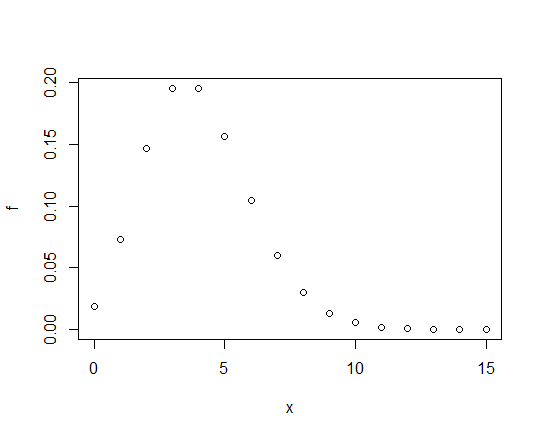
\includegraphics[height = 8cm]{dpois.png}
\captionof{figure}{Probability Mass Function of Poisson(4) Distribution.}
\end{center}

A mode of a distribution is a value which maximises the probability mass function. In the plot above, the mode of Poisson(4) would appear to be points 3 and 4. 

Respectively, median is a middle point of an organised set. In the context of probability distributions, meadian is the point $x$, for which
\[
P(X \leq x) \geq \frac{1}{2} \quad \text{ja} \quad P(X \geq x) \geq \frac{1}{2}.
\]

By examining the below graph of a cumulative density function, it would appear that the median would be $4$. The concept of median can be thought as if we were organising a finite data, which has been generated by the Poisson$(4)$ distribution. When we have gone through the numbers 0--3, we have handled circa 40\% of the whole data. Respectively, when we have gone through numbers 4 and 5, we have handled over 60 \% of the data. From this we infer that the median must be in between these two numbers, and since the value set is the set of non-negative intervals, the median must be $4$.

\begin{center}
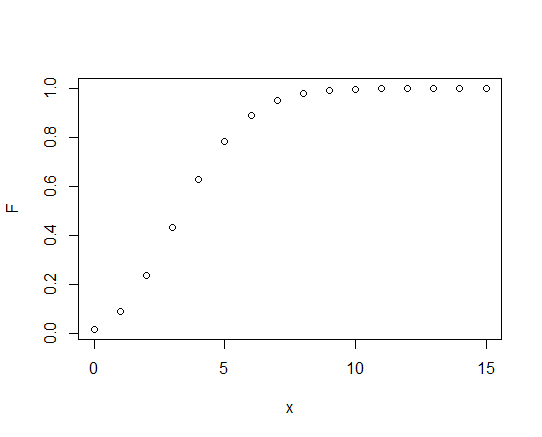
\includegraphics[height = 8cm]{ppois.png}
\captionof{figure}{Cumulative Density Function of Poisson(4) Distribution.}
\end{center}

Let us further strengthen our views by calculations.
\begin{verbatim}
max(f)
dpois(3, 4)
dpois(4, 4)

[1] 0.1953668
[1] 0.1953668
[1] 0.1953668

ppois(4, 4)
1 - ppois(3, 4)

[1] 0.6288369
[1] 0.5665299
\end{verbatim}

From the first set of lines we see that the maximum of the distribution equals the density at 3 and 4. Furthermore, the values of cumulative density function verify that
\[
P(X \leq 4) \approx 0.629 \quad \text{and} \quad P(X \geq 4) = 1 - P(X \leq 3) \approx 0.567,
\]
which makes 4 the median. The rightmost equality follows from the fact that $X$ can only attain values from the set of non-negative integers.
\end{esim}

We have now \emph{very} briefly introduced the reader to the world of R by showcasing random number generation, as well as some simple applications of our previously learned concepts. The following exercises include both R and analytical exercises, which will test broadly the concepts you have learned from this material, with a focus on the contents of the extra material section. Enjoy!

\section{Exercises}
\begin{enumerate}
\item Let $X \sim \text{Uni}(0,1)$. What is the probability that
\begin{enumerate}[(a)]
\item the first decimal of $\sqrt{X}$ is 3,
\item the first decimal of $X^2$ is 3.
\end{enumerate}
\item Let $X \sim \text{Exp}(1)$ and $Y = 5X$. Derve the cumulative density function and probability density function of $Y$, and identify its distribution.
\item Continued from examples \ref{esim:jpdf} ja \ref{esim:jpdf2}. Calculate 
\begin{enumerate}[(a)]
\item $P(X > 2, Y < 2)$,
\item $P(X > 5)$, and
\item $P(1 < X,Y < 3)$.
\end{enumerate}
\item (Ross Exercise 6.2) Random variables $X$, $Y$ and $Z$ have a joint distribution with a joint probability mass function of
\[
f(1,2,3) = f(3, 2, 1) = f(1, 1, 1) = f(2, 3, 2) = \frac{1}{4}.
\]
Find E(XYZ) and E(XY + XZ + YZ).
\item (Ross Problem 6.9) Random variables $X$ and $Y$ have a joint distribution with a joint probability mass function of
\[
f(x,y) = \frac{6}{7}\big(x^2 + \frac{xy}{2}\big), \quad \text{where } 0<x<1, \, 0<y<2.
\]
Calculate 
\begin{enumerate}[(a)]
\item $P(X < \frac{1}{2}, Y > 1)$,
\item E(X), and
\item E(Y).
\end{enumerate}
\item The following R code generates $n$ independent random numbers from $(0,1)$ interval, then multiplies them with $(b-a)$ and finally adds them $a$. A histogram is drawn for our newly generated and transformed numbers.
\begin{verbatim}
x = runif(n)
y = (b-a)*x+a
hist(y)
\end{verbatim}
\begin{enumerate}[(a)]
\item Try the code with parameter values $n = 10^6$, $a = 15$ and $b = 20$. What can you say about the distribution of the transformed numbers?
\item Edit the code such that the function to transform the numbers would be \verb|y = log(x)| (in R \verb|log| stands for the natural logarithm). What distribution the numbers appear to be following now?
\end{enumerate}
\end{enumerate}

\bigskip
\bigskip
\bigskip
\bigskip

That's it for the final set of exercises, and thus we have reached the end of the final section. Thank you for reading! I hope the material sparked some sense of clarity and enjoyment to the vast world of probabilites.

\bigskip

Writing the material was as enjoyable as ever, but sometimes amidst the most fun occasions, mistakes happen. Upon noticing a mistake or a suggestion for improvement, don't hesitate to email me at \emph{topias.tolonen@helsinki.fi}.

\printbibliography

\appendix
\chapter{Distribution Cheat Sheet}

\subsection*{Discrete Distributions}
\begin{tabular}{ l l L{90pt} l l l l}
\toprule
Distribution & Value Set & Parameters & Pmf $f_X(k)$ & $E(X)$ & $\var(X)$\\
\midrule
$\text{Bernoulli}(p)$ & $\{0,1\}$ & $p \in (0,1)$ & $p^k(1-p)^{1-k}$ & $p$ & $p(1-p)$\\\addlinespace[5pt]
$\text{Bin}(n,p)$ & $\{0,1, \dots, n\}$ & $n\in \N^+, p \in (0,1)$ & $\binom{n}{k} p^k(1-p)^{n-k}$ & $np$ & $np(1-p)$\\\addlinespace[5pt]
$\text{Geom}(p)$ & $\{0,1,2, \dots\}$ & $p \in (0,1)$ & $p(1-p)^k$ & $\frac{1-p}{p}$ & $\frac{1-p}{p^2}$\\\addlinespace[5pt]
$\text{Poisson}(\lambda)$ & $\{0,1,2, \dots\}$ & $\lambda > 0$ & $e^{-\lambda} \cdot \frac{\lambda^k}{k!}$ & $\lambda$ & $\lambda$\\ \addlinespace[5pt]
$\text{Hyperg}(N,K,n)$ & $\{0,1, \dots , n\}$ & $N,K,n \in\N^+$,   $n\leq N, \, K \leq N$ & $\frac{\binom{K}{k}\binom{N-K}{n-k}}{\binom{N}{n}}$ & $n\cdot\frac{K}{N}$ & $n\cdot\frac{K}{N}\cdot\frac{N-K}{N}\cdot\frac{N-n}{N-1}$\\
\bottomrule 
\end{tabular}

\bigskip

\subsection*{Continuous Distributions}
\begin{tabular}{ l l l l l l l}
\toprule
Distribution & Value Set & Parameters & Pdf $f_X(x)$ & $E(X)$ & $\var(X)$\\
\midrule
$\text{Uni}(a,b)$ & $(a,b)$ & $a,b \in \R,\, a < b$ & $\frac{1}{b-a}$ & $\frac{1}{2}(a+b)$ & $\frac{(b-a)^2}{12}$\\\addlinespace[5pt]
$\text{Exp}(\lambda)$ & $(0, \infty)$ & $\lambda > 0$ & $\lambda e^{-\lambda x}$ & $\frac{1}{\lambda}$ & $\frac{1}{\lambda^2}$\\\addlinespace[5pt]
$N(\mu, \sigma^2)$ & $\R$ & $\mu \in \R, \sigma^2 > 0$ & $\frac{1}{\sqrt{2\pi\sigma^2}} e^{-\frac{(x-\mu)^2}{2\sigma^2}}$ & $\mu$ & $\sigma^2$\\
\bottomrule 
\end{tabular}

\subsection*{Values for the Cumulative Density Function of the Standard Normal Distribution}
\begin{table}[ht]
	\centering
	\begin{tabular}{rrrrrrrrrrr}
		\hline
		$x$ & 0.00 & 0.01 & 0.02 & 0.03 & 0.04 & 0.05 & 0.06 & 0.07 & 0.08 & 0.09 \\ 
		\hline
		0.0 & 0.5000 & 0.5040 & 0.5080 & 0.5120 & 0.5160 & 0.5199 & 0.5239 & 0.5279 & 0.5319 & 0.5359 \\ 
		0.1 & 0.5398 & 0.5438 & 0.5478 & 0.5517 & 0.5557 & 0.5596 & 0.5636 & 0.5675 & 0.5714 & 0.5753 \\ 
		0.2 & 0.5793 & 0.5832 & 0.5871 & 0.5910 & 0.5948 & 0.5987 & 0.6026 & 0.6064 & 0.6103 & 0.6141 \\ 
		0.3 & 0.6179 & 0.6217 & 0.6255 & 0.6293 & 0.6331 & 0.6368 & 0.6406 & 0.6443 & 0.6480 & 0.6517 \\ 
		0.4 & 0.6554 & 0.6591 & 0.6628 & 0.6664 & 0.6700 & 0.6736 & 0.6772 & 0.6808 & 0.6844 & 0.6879 \\ 
		0.5 & 0.6915 & 0.6950 & 0.6985 & 0.7019 & 0.7054 & 0.7088 & 0.7123 & 0.7157 & 0.7190 & 0.7224 \\ 
		0.6 & 0.7257 & 0.7291 & 0.7324 & 0.7357 & 0.7389 & 0.7422 & 0.7454 & 0.7486 & 0.7517 & 0.7549 \\ 
		0.7 & 0.7580 & 0.7611 & 0.7642 & 0.7673 & 0.7704 & 0.7734 & 0.7764 & 0.7794 & 0.7823 & 0.7852 \\ 
		0.8 & 0.7881 & 0.7910 & 0.7939 & 0.7967 & 0.7995 & 0.8023 & 0.8051 & 0.8078 & 0.8106 & 0.8133 \\ 
		0.9 & 0.8159 & 0.8186 & 0.8212 & 0.8238 & 0.8264 & 0.8289 & 0.8315 & 0.8340 & 0.8365 & 0.8389 \\ 
		1.0 & 0.8413 & 0.8438 & 0.8461 & 0.8485 & 0.8508 & 0.8531 & 0.8554 & 0.8577 & 0.8599 & 0.8621 \\ 
		1.1 & 0.8643 & 0.8665 & 0.8686 & 0.8708 & 0.8729 & 0.8749 & 0.8770 & 0.8790 & 0.8810 & 0.8830 \\ 
		1.2 & 0.8849 & 0.8869 & 0.8888 & 0.8907 & 0.8925 & 0.8944 & 0.8962 & 0.8980 & 0.8997 & 0.9015 \\ 
		1.3 & 0.9032 & 0.9049 & 0.9066 & 0.9082 & 0.9099 & 0.9115 & 0.9131 & 0.9147 & 0.9162 & 0.9177 \\ 
		1.4 & 0.9192 & 0.9207 & 0.9222 & 0.9236 & 0.9251 & 0.9265 & 0.9279 & 0.9292 & 0.9306 & 0.9319 \\ 
		1.5 & 0.9332 & 0.9345 & 0.9357 & 0.9370 & 0.9382 & 0.9394 & 0.9406 & 0.9418 & 0.9429 & 0.9441 \\ 
		1.6 & 0.9452 & 0.9463 & 0.9474 & 0.9484 & 0.9495 & 0.9505 & 0.9515 & 0.9525 & 0.9535 & 0.9545 \\ 
		1.7 & 0.9554 & 0.9564 & 0.9573 & 0.9582 & 0.9591 & 0.9599 & 0.9608 & 0.9616 & 0.9625 & 0.9633 \\ 
		1.8 & 0.9641 & 0.9649 & 0.9656 & 0.9664 & 0.9671 & 0.9678 & 0.9686 & 0.9693 & 0.9699 & 0.9706 \\ 
		1.9 & 0.9713 & 0.9719 & 0.9726 & 0.9732 & 0.9738 & 0.9744 & 0.9750 & 0.9756 & 0.9761 & 0.9767 \\ 
		2.0 & 0.9772 & 0.9778 & 0.9783 & 0.9788 & 0.9793 & 0.9798 & 0.9803 & 0.9808 & 0.9812 & 0.9817 \\ 
		2.1 & 0.9821 & 0.9826 & 0.9830 & 0.9834 & 0.9838 & 0.9842 & 0.9846 & 0.9850 & 0.9854 & 0.9857 \\ 
		2.2 & 0.9861 & 0.9864 & 0.9868 & 0.9871 & 0.9875 & 0.9878 & 0.9881 & 0.9884 & 0.9887 & 0.9890 \\ 
		2.3 & 0.9893 & 0.9896 & 0.9898 & 0.9901 & 0.9904 & 0.9906 & 0.9909 & 0.9911 & 0.9913 & 0.9916 \\ 
		2.4 & 0.9918 & 0.9920 & 0.9922 & 0.9925 & 0.9927 & 0.9929 & 0.9931 & 0.9932 & 0.9934 & 0.9936 \\ 
		2.5 & 0.9938 & 0.9940 & 0.9941 & 0.9943 & 0.9945 & 0.9946 & 0.9948 & 0.9949 & 0.9951 & 0.9952 \\ 
		2.6 & 0.9953 & 0.9955 & 0.9956 & 0.9957 & 0.9959 & 0.9960 & 0.9961 & 0.9962 & 0.9963 & 0.9964 \\ 
		2.7 & 0.9965 & 0.9966 & 0.9967 & 0.9968 & 0.9969 & 0.9970 & 0.9971 & 0.9972 & 0.9973 & 0.9974 \\ 
		2.8 & 0.9974 & 0.9975 & 0.9976 & 0.9977 & 0.9977 & 0.9978 & 0.9979 & 0.9979 & 0.9980 & 0.9981 \\ 
		2.9 & 0.9981 & 0.9982 & 0.9982 & 0.9983 & 0.9984 & 0.9984 & 0.9985 & 0.9985 & 0.9986 & 0.9986 \\ 
		3.0 & 0.9987 & 0.9987 & 0.9987 & 0.9988 & 0.9988 & 0.9989 & 0.9989 & 0.9989 & 0.9990 & 0.9990 \\ 
		\hline
	\end{tabular}
\end{table}

\printindex

\end{document}